\title{Buku Tugas Akhir ITS}
\author{Imanuel Daulat Satrio Utomo Siahaan}
% Pengaturan ukuran teks dan bentuk halaman dua sisi
\documentclass[12pt,twoside]{report}
\input{Init/Init.tex}
%========================================
%Template ini di modifikasi oleh departement Teknik Komputer ITS
%dari template yang telah dibuat Musk, Elon Reeve
%=======================================

%=======================================
%Direktori Penting 
%1. Init : Berisi File penting terkait dengan konfigurasi .
%            Isi dari direktori ini jangan diubah
%2.KataPengantar 
%3. Abstrak : berisi abstrak untuk bahasa indonesia dan bahasa inggris 
%4. Bab1-Bab5 : Isi tiap-tiap bab
%5. Pustaka : Berisi daftar pustaka 
%6. Biografi penulis 
%=======================================

%========================================
% Identutas Mahasiswa} 
%========================================
\NamaMahasiswa{Imanuel Daulat Satrio Utomo Siahaan}{5024 22 1066}

%========================================
%Identitas Tugas Akhir
%========================================
\KodeMataKuliah{EC234801}
\JudulTAInd{PERANCANGAN DAN IMPLEMENTASI PIPELINE \textit{MACHINE LEARNING OPERATIONS} (MLOps) UNTUK OPERASIONALISASI MODEL PREDIKTIF RISIKO KREDIT}
\JudulTAEng{DESIGN AND IMPLEMENTATION OF A \textit{MACHINE LEARNING OPERATIONS} (MLOps) PIPELINE FOR THE OPERATIONALIZATION OF CREDIT RISK PREDICTIVE MODELS}
\Tempat{Surabaya}

%========================================
% Daftar Pembimbing 
%========================================
\PembimbingSatu{Reza Fuad Rachmadi, S.T., M.T., Ph.D}{19850403201212 1 001} 
\PembimbingDua{Dr. Surya Sumpeno, S.T., M.Sc.}{19690613199702 1 003}

%========================================
% Daftar Penguji
%========================================
\PengujiSatu{Dr. Supeno Mardi Susiki N., S.T., M.T.}{19700313199512 1 001} 
\PengujiDua{Dr. Susi Juniastuti, S.T., M.Eng.}{19650618199903 2 001} 
%Tambahkan dosen penguji 3
%\PengujiTiga{Arta Kusuma Hernanda, S.T., M.T.}{1996202311024} 


%========================================
%Identitas Departement dan fakultas
%========================================
\KepalaDepartemen{Dr. Arief Kurniawan, S.T., M.T.}{19740907200212 1 001} 
\Departemen{Teknik Komputer}{Computer Engineering}
\Fakultas{Teknologi Elektro dan Informatika Cerdas}{Intelligent Electrical And Informatics Technology}
\SingkatanFakultas{FTEIC}{FIEI}


% Isi keseluruhan dokumen
\begin{document}
\input{Init/TataLetak.tex} 

% Bab 1 pendahuluan

\begin{spacing}{1.2}
  \chapter{PENDAHULUAN}
\end{spacing}


\pagenumbering{arabic}
\vspace{4ex}

\section{Latar Belakang}
Penelitian ini dilatarbelakangi oleh meningkatnya kebutuhan lembaga keuangan terhadap sistem analisis risiko kredit yang lebih adaptif, akurat, dan dapat dikelola secara berkelanjutan. Perkembangan pesat di bidang kecerdasan buatan, khususnya Machine Learning (ML), telah menghadirkan peluang baru dalam penilaian kelayakan kredit, baik bagi individu maupun perusahaan. Namun, penerapan ML dalam konteks analisis risiko menghadapi tantangan besar pada tahap operasional dan pemeliharaan model di lingkungan produksi. Untuk menjawab tantangan tersebut, muncul konsep Machine Learning Operations (MLOps) yang menggabungkan prinsip DevOps dengan proses pengembangan, penerapan, serta pengawasan model ML secara berkelanjutan.\cite{google2024mlops}

Perkembangan teknologi finansial di Indonesia telah mendorong transformasi signifikan dalam cara lembaga keuangan menilai risiko kredit. Baik bank konvensional maupun perusahaan financial technology (fintech) kini bergantung pada analisis data untuk menentukan tingkat risiko calon peminjam. Berdasarkan laporan Otoritas Jasa Keuangan (OJK), nilai penyaluran pinjaman fintech lending pada tahun 2024 mencapai lebih dari Rp55 triliun per bulan, dengan jumlah rekening peminjam yang terus meningkat. Namun, di balik pertumbuhan tersebut, risiko gagal bayar (credit default) juga meningkat, sebagaimana tercermin dari rasio Non-Performing Loan (NPL) sektor keuangan yang masih berada di kisaran 2,5 - 3 persen.\cite{ojk2024pojk29} Kondisi ini menunjukkan pentingnya penguatan sistem analisis risiko kredit yang mampu menyesuaikan diri terhadap dinamika ekonomi dan perilaku nasabah.

Model Machine Learning banyak digunakan dalam analisis risiko kredit karena kemampuannya mempelajari pola dari data historis, perilaku transaksi, hingga variabel eksternal seperti kondisi makroekonomi. Model ini dapat memprediksi probabilitas gagal bayar (default probability) calon debitur dengan lebih cepat dan akurat dibandingkan metode tradisional.\cite{mlopsfinance2025} Namun, permasalahan utama muncul ketika model tersebut diterapkan dalam jangka panjang: performa model dapat menurun seiring waktu sehingga model menjadi usang (stale model), sulit dimonitor secara konsisten, serta tidak memiliki proses pembaruan otomatis. Akibatnya, keputusan kredit menjadi kurang andal dan berpotensi menimbulkan kerugian finansial. Konsep MLOps hadir untuk mengatasi permasalahan tersebut. MLOps menerapkan prinsip DevOps pada siklus hidup model ML, mulai dari tahap data ingestion, training, deployment, monitoring, hingga retraining. Dengan penerapan MLOps, model analisis risiko dapat diperbarui secara otomatis, kinerjanya dimonitor secara berkelanjutan, serta proses audit dan dokumentasinya lebih terjamin. Penelitian ini berfokus pada perancangan dan implementasi pipeline MLOps untuk operasionalisasi model prediktif risiko kredit menggunakan dataset sintetis, transformasi Weight of Evidence (WoE), seleksi Information Value (IV), model XGBoost, layanan inferensi FastAPI, interpretasi SHAP, serta otomasi pelatihan ulang berkelanjutan (Continuous Training) melalui n8n. \cite{mlopsbanking2025}

\section{Rumusan Masalah}
Dari latar belakang yang telah dijelaskan, dapat diidentifikasi beberapa permasalahan utama sebagai berikut:
\begin{enumerate}
    \item Belum adanya sistem otomatis yang dapat mengelola dan memantau model Machine Learning untuk analisis risiko kredit secara berkelanjutan.
    \item Kurangnya penerapan konsep MLOps pada sistem analisis risiko kredit di lingkungan perbankan Indonesia, terutama pada proses pembaruan model (retraining) dan pemantauan performa (monitoring).
    \item Belum tersedia arsitektur pipeline MLOps berbasis low-code yang mengintegrasikan validasi data sintetis, pelacakan eksperimen, deployment API, interpretabilitas model, aturan bisnis, serta pelatihan ulang otomatis (Continuous Training) untuk sistem analisis risiko kredit.
\end{enumerate}
\section{Tujuan}
Tujuan dari penelitian ini adalah:
\begin{enumerate}
    \item Merancang arsitektur sistem analisis risiko kredit yang terintegrasi dengan konsep Machine Learning Operations (MLOps).
    \item Mengembangkan pipeline otomatis yang mencakup pembentukan dan validasi data sintetis, pra-pemrosesan WoE-IV, penanganan ketidakseimbangan kelas, pelatihan XGBoost, pelacakan eksperimen, deployment API, dan otomasi Continuous Training.
    \item Mengevaluasi performa model dan kesiapan operasional pipeline melalui metrik prediktif, quality gate data sintetis, interpretasi SHAP, pengujian aturan bisnis, serta pemicuan retraining berbasis n8n.
\end{enumerate}
\section{Batasan Masalah}
Batasan dalam penelitian ini adalah sebagai berikut:
\begin{enumerate}
    \item Penelitian difokuskan pada penerapan MLOps dalam konteks analisis risiko kredit, tanpa membahas pengembangan algoritma machine learning baru.
    \item Dataset yang digunakan merupakan dataset sintetis yang dirancang untuk merepresentasikan karakteristik umum data kredit konsumtif, bukan data nasabah riil dari lembaga keuangan tertentu.
    \item Implementasi dilakukan pada lingkungan pengujian lokal menggunakan Python, XGBoost, Scikit-Learn, Imbalanced-Learn, MLflow, FastAPI, Docker, Docker Compose, SHAP, dan n8n sebagai workflow orchestration tool.
    \item Penelitian ini tidak melibatkan data atau kerja sama langsung dengan lembaga keuangan tertentu.
    \item Fokus penelitian adalah pada perancangan pipeline MLOps, evaluasi performa model, validasi kualitas data sintetis, deployment layanan inferensi, penerapan aturan bisnis, serta implementasi Continuous Training.
\end{enumerate}

\section{Manfaat}
Manfaat dari penelitian ini adalah:
\subsection*{Manfaat Akademis} Penelitian ini dapat menjadi referensi bagi pengembangan ilmu pengetahuan di bidang Machine Learning Operations (MLOps), khususnya dalam penerapan teknologi tersebut untuk sistem analisis risiko kredit. Hasil penelitian juga dapat menjadi contoh implementasi pipeline MLOps menggunakan low-code workflow tool seperti n8n dengan data sintetis yang menggambarkan karakteristik umum data kredit konsumtif.
\subsection*{Manfaat Teknis} Penelitian ini menghasilkan rancangan dan implementasi arsitektur MLOps berbasis n8n yang dapat digunakan sebagai acuan dalam membangun sistem analisis risiko kredit yang efisien dan berkelanjutan. Pipeline mencakup proses validasi data sintetis, preprocessing WoE-IV, training, deployment API, interpretasi model, serta pelatihan ulang model secara otomatis (Continuous Training).
\subsection*{Manfaat Praktis} Meskipun penelitian ini tidak dilakukan secara langsung di lembaga keuangan tertentu, hasilnya dapat dijadikan prototipe atau simulasi bagi bank maupun perusahaan fintech yang ingin mengadopsi MLOps dengan pendekatan low-code, layanan inferensi berbasis API, dan aturan bisnis yang dapat diaudit.
\subsection*{Manfaat Sosial dan Industri} Secara tidak langsung, penelitian ini berkontribusi terhadap peningkatan praktik tata kelola model machine learning di sektor keuangan Indonesia melalui penerapan konsep MLOps yang transparan, adaptif, dan sesuai dengan prinsip akuntabilitas yang ditekankan oleh OJK dan Bank Indonesia.


\cleardoublepage
\chapter{KAJIAN PUSTAKA}


\section{Hasil Penelitian/Perancangan Terdahulu}
Penelitian ini mengacu pada beberapa penelitian terdahulu yang relevan sebagai dasar pengembangan dan pembanding dalam menentukan celah penelitian (\textit{research gap}). Referensi utama yang digunakan meliputi studi mengenai \textit{Machine Learning} dalam analisis risiko kredit serta implementasi \textit{Machine Learning Operations} (MLOps), yang diuraikan sebagai berikut.\cite{Chang2024, sharma2021default}.


\subsection{\textit{Research gap} dari Penelitian Terdahulu }

\begin{figure}[H]
    \centering
    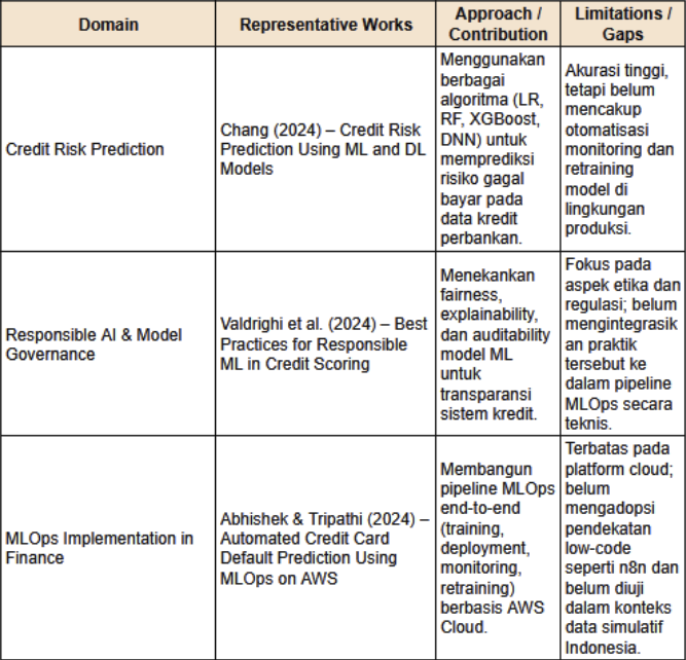
\includegraphics[width=0.8\textwidth]{bab2/Research_gap.png}
    \caption{\textit{Research gap} dari penelitian terdahulu}
    \label{fig:Research gap}
\end{figure}
\subsection*{1. Dasar Pemilihan Model \textit{Machine Learning}}
\textbf{Credit Risk Prediction Using Machine Learning and Deep Learning Models}
Penelitian tersebut mengkaji penerapan berbagai algoritma \textit{Machine Learning}, seperti Logistic Regression, Random Forest, XGBoost, dan Deep Neural Network, untuk memprediksi risiko gagal bayar pada data kredit perbankan. Hasil penelitian menunjukkan bahwa model berbasis \textit{ensemble learning} seperti XGBoost memiliki performa yang stabil dalam mendeteksi potensi gagal bayar nasabah. Temuan ini menjadi dasar pemilihan algoritma \textit{Machine Learning} yang digunakan dalam sistem analisis risiko kredit pada penelitian ini.\cite{sharma2021default}

\textbf{Credit Scoring Using Machine Learning and Deep Learning Techniques}
Penelitian ini merupakan studi komparatif terhadap beberapa algoritma pembelajaran mesin (SVM, LDA, DNN) untuk proses \textit{credit scoring}. Studi tersebut menekankan pentingnya pemrosesan data awal, seperti normalisasi dan penanganan ketidakseimbangan kelas (\textit{class imbalance}) pada \textit{dataset} kredit. Relevansinya adalah bahwa performa model yang dikelola dalam \textit{pipeline} MLOps sangat bergantung pada langkah pra-pemrosesan data (\textit{data preprocessing}) dan pemilihan model yang tepat.\cite{creditscoringml2024}

\subsection*{2. Justifikasi Kebutuhan \textit{Machine Learning Operations} (MLOps)}
\textbf{Automated Credit Card Default Prediction Using MLOps on AWS}
Penelitian memperkenalkan implementasi MLOps untuk prediksi gagal bayar kartu kredit menggunakan layanan AWS. \textit{Pipeline} yang dikembangkan mencakup tahapan \textit{model training, deployment, monitoring}, hingga \textbf{retraining otomatis} dengan integrasi CI/CD. Penelitian ini membuktikan bahwa penerapan MLOps dapat \textbf{mempercepat proses \textit{deployment} model hingga tiga kali lipat} dan menurunkan waktu \textit{downtime} model sebesar 40\%. Hasil ini memperkuat dasar bahwa integrasi MLOps sangat efektif dan diperlukan untuk menjaga performa model analisis risiko kredit di lingkungan produksi.\cite{creditscoringml2024}

\textbf{MLOps: Continuous Delivery and Automation Pipelines in Machine Learning}
Laporan teknis ini menjelaskan arsitektur dan praktik terbaik dalam implementasi MLOps, mencakup \textit{continuous integration}, \textit{continuous delivery}, \textit{model registry}, \textit{monitoring}, dan \textit{automated retraining}. Penelitian ini relevan karena memberikan gambaran arsitektur MLOps yang bersifat umum. Arsitektur tersebut kemudian diadaptasi dalam penelitian ini menggunakan \textit{low-code tool} n8n untuk mengatur \textit{pipeline} analisis risiko kredit otomatis berbasis data simulatif.\cite{Kreuzberger2023}

\subsection*{3. Aspek Regulasi dan Tata Kelola Model}
\textbf{Best Practices for Responsible Machine Learning in Credit Scoring}
Studi ini mengusulkan panduan penerapan \textit{Responsible AI} dalam konteks \textit{credit scoring} yang menyoroti aspek \textit{fairness}, \textit{explainability}, dan \textit{auditability} model. Penelitian ini menekankan bahwa sistem berbasis ML di sektor keuangan harus memiliki \textit{audit trail} dan dokumentasi yang jelas untuk memastikan transparansi keputusan kredit. Temuan ini menjadi rujukan penting dalam pengembangan \textit{pipeline} MLOps yang menjamin tata kelola (\textit{governance}) dan kepatuhan terhadap regulasi OJK dan Bank Indonesia.\cite{Valdrighi2024}

\subsection*{4. Pentingnya Pra-pemrosesan Data}
Berbagai studi komparatif mengenai \textit{credit scoring} menunjukkan bahwa performa prediktif model ML sangat bergantung pada kualitas data awal, terlepas dari kompleksitas algoritmanya. Langkah pra-pemrosesan yang andal penting, terutama dalam menangani ketidakseimbangan kelas (\textit{class imbalance}). Pada \textit{dataset} kredit, kasus gagal bayar (\textit{default}) umumnya merupakan kelas minoritas sehingga teknik penyeimbangan khusus diperlukan. Teknik seperti \textit{Synthetic Minority Over-sampling Technique} (SMOTE) membantu model ML mendeteksi pola \textit{default} secara lebih efektif. Keandalan langkah pra-pemrosesan ini secara langsung memengaruhi stabilitas model yang akan dioperasionalkan dalam \textit{pipeline} MLOps.
MLOps memainkan peran krusial dalam domain keuangan yang sangat teregulasi. Sistem MLOps yang terstruktur memungkinkan otomatisasi proses kepatuhan (\textit{compliance}) dan tata kelola (\textit{governance}). MLOps menyediakan kerangka kerja untuk memublikasikan, memantau, dan melatih ulang model secara teratur dengan menerapkan prinsip CI/CD. Prinsip tersebut menjamin konsistensi, akuntabilitas, dan auditabilitas yang menjadi tuntutan utama regulator seperti Otoritas Jasa Keuangan (OJK) dan Bank Indonesia.\cite{AIMSPress2024}
\subsection*{5. Fungsi Tata Kelola Keuangan}
MLOps memainkan peran krusial dalam domain keuangan yang sangat teregulasi. Sistem MLOps yang terstruktur memungkinkan otomatisasi proses kepatuhan (\textit{compliance}) dan tata kelola (\textit{governance}). MLOps menyediakan kerangka kerja untuk memublikasikan, memantau, dan melatih ulang model secara teratur dengan menerapkan prinsip CI/CD. Prinsip tersebut menjamin konsistensi, akuntabilitas, dan auditabilitas yang menjadi tuntutan utama regulator seperti Otoritas Jasa Keuangan (OJK) dan Bank Indonesia.\cite{rafi2024explainable}

\subsection*{6. Analisis Kesenjangan Penelitian (Research Gap)}

Berdasarkan telaah terhadap penelitian-penelitian terdahulu, dapat diidentifikasi bahwa mayoritas studi mengenai analisis risiko kredit berbasis \textit{Machine Learning} berfokus pada peningkatan akurasi model prediksi, khususnya melalui penggunaan algoritma \textit{ensemble learning} seperti XGBoost, Random Forest, dan Deep Neural Network.\cite {Chang2024} Namun demikian, sebagian besar penelitian tersebut masih menitikberatkan pada tahap eksperimentasi model (\textit{offline modeling}) dan belum membahas secara komprehensif aspek operasionalisasi model di lingkungan produksi.

Selain itu, penelitian terkait \textit{Machine Learning Operations} (MLOps) umumnya mengadopsi arsitektur berbasis \textit{cloud-native} atau \textit{hyperscale platform} seperti AWS, Azure, atau Kubeflow, yang memerlukan sumber daya infrastruktur dan kompetensi teknis tingkat lanjut. Pendekatan tersebut relatif sulit diadopsi oleh organisasi berskala kecil hingga menengah, khususnya dalam konteks industri keuangan di Indonesia yang memiliki keterbatasan sumber daya teknis.\cite{GoogleCloud2024}

Kesenjangan penelitian lainnya terletak pada minimnya kajian yang mengeksplorasi penggunaan \textbf{platform low-code} sebagai orkestrator utama dalam pipeline MLOps. Penelitian yang secara spesifik mengintegrasikan proses \textit{training, deployment, monitoring}, dan \textit{automated retraining} menggunakan alat \textit{low-code} seperti \textbf{n8n} masih sangat terbatas.

Berdasarkan hal tersebut, penelitian ini bertujuan mengisi celah tersebut dengan merancang dan mengimplementasikan \textit{pipeline} MLOps berbasis \textit{low-code} untuk analisis risiko kredit. Pipeline ini mengintegrasikan model \textit{Machine Learning} (XGBoost), \textit{model registry}, \textit{containerization}, serta mekanisme \textit{monitoring} dan \textit{continuous training} secara otomatis. Pendekatan ini diharapkan menjadi solusi yang lebih praktis, efisien, dan mudah direplikasi dalam konteks operasional lembaga keuangan di Indonesia. \cite{Sundberg2023}


\section{Teori/Konsep Dasar}

\subsection{Pra-Pemrosesan Data Lanjutan dalam Credit Scoring}

Selain teknik normalisasi dan penyeimbangan kelas, pemodelan risiko kredit juga memerlukan pendekatan pra-pemrosesan yang berfokus pada stabilitas dan interpretabilitas fitur. Salah satu teknik yang banyak digunakan dalam industri perbankan adalah transformasi \textit{Weight of Evidence} (WoE) dan pengukuran \textit{Information Value} (IV).\cite{venkatsai2025validation}

Transformasi WoE dilakukan dengan mendiskretisasi variabel numerik ke dalam beberapa \textit{bin}, kemudian menghitung rasio logaritmik antara proporsi debitur baik (\textit{non-default}) dan debitur gagal bayar (\textit{default}) pada setiap bin. Pendekatan ini menghasilkan fitur yang lebih stabil dan mudah diinterpretasikan, bahkan ketika digunakan pada model \textit{black-box} seperti XGBoost.\cite{ye2025unlocking}

Sementara itu, \textit{Information Value} (IV) digunakan sebagai metrik seleksi fitur untuk mengukur kekuatan prediktif suatu variabel terhadap risiko gagal bayar. Variabel dengan nilai IV yang sangat rendah dianggap tidak informatif, sedangkan nilai IV yang terlalu tinggi dapat mengindikasikan potensi \textit{data leakage}.\cite{maurino2025data}

Penggunaan WoE dan IV memiliki relevansi langsung dengan implementasi MLOps, karena fitur yang lebih stabil mempermudah proses pemantauan \textit{data drift}. Dalam konteks ini, perubahan distribusi fitur WoE dapat dideteksi secara kuantitatif menggunakan metrik seperti \textit{Population Stability Index} (PSI), yang selanjutnya digunakan sebagai pemicu proses \textit{retraining} otomatis dalam pipeline MLOps.\cite{Chang2024}


\subsection{Analisis Risiko Kredit}
Analisis risiko kredit merupakan proses penilaian kemampuan calon nasabah dalam memenuhi kewajiban pembayaran pinjaman. Tujuan utama analisis risiko kredit adalah untuk meminimalkan kemungkinan terjadinya \textbf{gagal bayar (\textit{credit default})}. Secara tradisional, lembaga keuangan menggunakan pendekatan analisis 5C (\textit{Character, Capacity, Capital, Condition, Collateral}). Namun pendekatan ini sering kali bersifat subjektif dan kurang adaptif. Dengan kemajuan \textit{Machine Learning}, proses penilaian risiko kredit dapat dilakukan lebih otomatis dan akurat melalui analisis data historis dan pola transaksi. \cite{ojk2024pojk29}
\subsection{Kalkulasi Risiko Kredit}
Kalkulasi risiko kredit adalah proses kuantifikasi potensi kerugian finansial yang dapat dialami lembaga keuangan akibat gagal bayar debitur. Salah satu metrik utama dalam manajemen risiko kredit adalah \textit{Expected Loss} (EL), yang dihitung sebagai:

\[
\text{EL} = \text{PD} \times \text{LGD} \times \text{EAD} 
\]
\begin{itemize}
    \item \textbf{PD (\textit{Probability of Default})}: Probabilitas bahwa debitur akan gagal memenuhi kewajiban pembayaran dalam periode tertentu. Nilai ini merupakan target utama prediksi dari model \textit{Machine Learning}.
    \item \textbf{LGD (\textit{Loss Given Default})}: Persentase kerugian yang dialami bank jika debitur gagal bayar.
    \item \textbf{EAD (\textit{Exposure at Default})}: Total nilai pinjaman yang terekspos saat gagal bayar terjadi.
\end{itemize}
Dengan mengotomatisasi perhitungan PD dan memantau performa model yang menghasilkan nilai tersebut, penerapan MLOps dapat meningkatkan akurasi dan keandalan kalkulasi risiko kredit.\cite{Chang2024}

\subsection{\textit{Machine Learning} dalam Analisis Risiko Kredit}
\textit{Machine Learning} memungkinkan pembangunan model \textit{credit scoring} yang secara otomatis mengklasifikasikan calon debitur ke dalam kategori “layak” atau “berisiko”. Algoritma yang sering digunakan antara lain:
\begin{itemize}
    \item Logistic Regression
    \item Random Forest dan XGBoost
    \item Neural Network
\end{itemize}
Model \textit{ensemble} seperti XGBoost dapat meningkatkan akurasi prediksi.\cite{mlopsbanking2025}

\subsection{Credit Scoring dan Model Drift}
\textbf{\textit{Model drift}} adalah penurunan performa model akibat perubahan distribusi data. Dua jenis \textit{drift} utama yang relevan dalam \textit{credit scoring} adalah:
\begin{itemize}
    \item \textbf{\textit{Data drift}}: perubahan pada distribusi input (misalnya, perubahan demografi nasabah).
    \item \textbf{\textit{Concept drift}}: perubahan hubungan antara input dan target (misalnya, krisis ekonomi mengubah perilaku gagal bayar).
\end{itemize}
MLOps diperlukan untuk mengatasi masalah ini melalui mekanisme \textit{monitoring}, \textit{alerting}, dan \textit{retraining} model secara otomatis. \cite{nikolaidis2022credit}

\subsection{Evaluasi Kinerja Model dan Transformasi ke Keputusan Operasional}

Evaluasi kinerja model prediksi risiko kredit tidak hanya berfokus pada akurasi global, tetapi juga pada kemampuan model dalam membedakan debitur berisiko tinggi dan rendah. Oleh karena itu, metrik evaluasi yang umum digunakan meliputi \textit{Area Under the Curve} (AUC), \textit{F1-Score}, dan \textit{Kolmogorov-Smirnov (K-S) Statistic}.\cite{venkatsai2025validation}

Statistik K-S memiliki peran penting dalam konteks operasional, karena digunakan untuk menentukan ambang batas (\textit{cut-off}) skor kredit yang optimal. Ambang batas ini merepresentasikan titik pemisahan maksimum antara distribusi probabilitas debitur baik dan debitur gagal bayar, sehingga dapat diterjemahkan secara langsung menjadi kebijakan kredit.

Output model berupa nilai \textit{Probability of Default} (PD) selanjutnya ditransformasikan ke dalam bentuk \textit{credit scorecard} dan \textit{risk grade} institusional. Proses ini memungkinkan hasil prediksi model untuk diintegrasikan secara otomatis ke dalam sistem pengambilan keputusan kredit, seperti keputusan \textit{approve}, \textit{reject}, atau \textit{manual review}, yang diorkestrasi melalui pipeline MLOps.\cite{nikolaidis2022credit,mlopsdrift2025}


\subsection{Konsep \textit{Machine Learning Operations} (MLOps)}
MLOps merupakan integrasi DevOps dengan siklus hidup \textit{Machine Learning} (\textit{training}, \textit{deployment}, \textit{monitoring}, \textit{retraining}). Komponen utama MLOps meliputi:
\begin{itemize}
    \item Data Pipeline
    \item Model Pipeline
    \item Deployment Pipeline
    \item Monitoring \& Retraining
\end{itemize}
\textbf{CI (\textit{Continuous Integration})}, \textbf{CD (\textit{Continuous Delivery})}, dan \textbf{CT (\textit{Continuous Training})} adalah fondasi utama dari MLOps.\cite{Nogare2023}

\subsection{Explainable AI (XAI) dan Kepatuhan Regulasi}

Dalam sektor keuangan yang sangat teregulasi, model \textit{Machine Learning} tidak hanya dituntut memiliki performa tinggi, tetapi juga harus dapat dijelaskan (\textit{explainable}) dan dapat diaudit. Regulasi menuntut lembaga keuangan untuk mampu memberikan alasan yang jelas atas setiap keputusan kredit, khususnya pada kasus penolakan pinjaman.

Model \textit{ensemble learning} seperti XGBoost bersifat \textit{black-box} moderat, sehingga memerlukan metode penjelasan pasca-pelatihan (\textit{post-hoc explanation}). Salah satu pendekatan yang paling banyak digunakan adalah \textit{SHapley Additive exPlanations} (SHAP), yang mampu memberikan penjelasan baik secara lokal (tingkat individu) maupun global (tingkat model).\cite{yotsawat2021improved}

Integrasi XAI ke dalam pipeline MLOps memungkinkan setiap prediksi kredit tidak hanya menghasilkan nilai PD, tetapi juga disertai dengan penjelasan kontribusi fitur. Informasi ini dicatat sebagai bagian dari \textit{audit trail}, sehingga mendukung aspek transparansi, akuntabilitas, dan kepatuhan regulasi terhadap ketentuan Otoritas Jasa Keuangan (OJK) dan Bank Indonesia.\cite{ye2025unlocking}

\subsection{Low-Code Workflow Automation (n8n)}
n8n adalah \textit{tool} \textit{low-code} yang digunakan untuk mengotomatisasi \textit{workflow} secara visual. Dengan n8n, \textit{pipeline} MLOps dapat dibangun tanpa \textit{scripting} yang kompleks. Pendekatan ini mencakup tahapan \textit{data preparation, training, deployment,} dan \textit{alerting}. Pendekatan \textit{low-code} ini cocok untuk organisasi kecil-menengah dan relevan dengan penelitian ini yang bertujuan merancang \textit{pipeline} MLOps yang efisien.\cite{Sundberg2023}




\cleardoublepage
\chapter{METODOLOGI}

\section{Metodologi Penelitian}

\noindent Bab ini menguraikan tahapan metodologi, kerangka desain, dan arsitektur sistem untuk pengembangan model \textit{Credit Risk Scoring} terautomasi dengan integrasi prinsip \textit{Machine Learning Operations} (MLOps)[cite: 3]. Fokus utama sistem ini adalah mengatasi tantangan \textit{data drift} dan \textit{concept drift} secara \textit{real-time}[cite: 4]. Secara umum, metodologi penelitian dirancang untuk memastikan bahwa proses pengembangan model tidak berhenti pada tahap eksperimen, tetapi berlanjut hingga implementasi, pemantauan, dan perbaikan model secara berkesinambungan. Dengan demikian, penelitian ini tidak hanya menghasilkan model prediktif, namun juga menghasilkan kerangka kerja operasional yang siap diterapkan pada lingkungan produksi.

Pendekatan yang digunakan adalah \textit{applied research}, yaitu penelitian terapan yang berorientasi pada penyelesaian masalah nyata melalui perancangan, pembangunan, dan evaluasi sistem[cite: 7, 8]. Permasalahan utama yang diangkat adalah kebutuhan akan sistem penilaian risiko kredit yang akurat, dapat dijelaskan, dan berkelanjutan. Ketiga aspek tersebut menjadi krusial ketika distribusi data berubah seiring waktu. Oleh karena itu, metodologi penelitian ini mengintegrasikan rekayasa data, pengembangan model, evaluasi kualitas data sintetis, serta otomasi proses MLOps dalam satu alur kerja terpadu.


\subsection{Tahapan Penelitian}
Tahapan penelitian disusun secara berurutan agar setiap proses memiliki keluaran yang menjadi masukan bagi tahap berikutnya. Secara garis besar, penelitian ini terdiri atas enam tahap utama, yaitu: (1) perumusan kebutuhan sistem dan identifikasi variabel penelitian, (2) pengumpulan serta simulasi data, (3) pra-pemrosesan dan rekayasa fitur, (4) pelatihan dan evaluasi model, (5) validasi kualitas data sintetis, dan (6) implementasi \textit{pipeline} MLOps untuk \textit{deployment}, \textit{monitoring}, dan \textit{retraining} otomatis. Urutan tahapan ini dipilih agar kualitas model dan kesiapan operasional dievaluasi sejak awal sebelum sistem diimplementasikan secara penuh.

Pada tahap pertama, kebutuhan sistem diidentifikasi berdasarkan karakteristik umum proses analisis risiko kredit pada lembaga keuangan. Pada tahap ini, tujuan model ditetapkan, target prediksi didefinisikan, kendala regulasi diidentifikasi, dan kebutuhan interpretabilitas model ditentukan. Tahap kedua berfokus pada penyusunan dataset sintetis yang merepresentasikan profil nasabah. Tahap ketiga mencakup transformasi data mentah menjadi fitur yang siap dipelajari model. Tahap keempat memusatkan perhatian pada pelatihan model \textit{machine learning}, optimasi parameter, dan evaluasi performa. Tahap kelima berfungsi sebagai \textit{quality gate} untuk memastikan data sintetis memiliki utilitas dan keamanan yang memadai. Tahap keenam mengintegrasikan seluruh komponen ke dalam arsitektur MLOps sehingga model dapat dioperasikan secara berkelanjutan.

\subsection{Desain Sistem dan Arsitektur Penelitian}
Arsitektur sistem dirancang menggunakan pendekatan \textit{pipeline machine learning end-to-end} yang bersifat modular[cite: 9]. Modularitas ini memungkinkan setiap komponen dikembangkan, diuji, dan dipelihara secara terpisah. Pemisahan tersebut mendukung skalabilitas sistem, mempermudah pelacakan eksperimen, serta mengurangi ketergantungan antarproses ketika terjadi pembaruan model atau perubahan data.

Secara konseptual, arsitektur penelitian terdiri atas empat lapisan utama. Lapisan pertama adalah \textit{data layer} yang menangani pembentukan data sintetis, validasi struktur data, dan penyimpanan dataset kerja. Lapisan kedua adalah \textit{modeling layer} yang mencakup transformasi fitur, pelatihan model, evaluasi kinerja, dan penyimpanan artefak model. Lapisan ketiga adalah \textit{quality assurance layer} yang memastikan bahwa dataset sintetis memenuhi kriteria utilitas dan privasi sebelum digunakan lebih lanjut. Lapisan keempat adalah \textit{MLOps layer} yang bertugas mengelola orkestrasi \textit{workflow}, registrasi model, \textit{deployment} layanan inferensi, pemantauan \textit{drift}, dan \textit{retraining} otomatis.

\begin{table}[H]
\centering
\caption{Komponen Arsitektur dan Teknologi}
\label{tab:arsitektur}
\begin{tabularx}{\textwidth}{|p{3.2cm}|X|p{4cm}|}
\hline
\textbf{Komponen} & \textbf{Deskripsi} & \textbf{Teknologi} \\ \hline
\textit{Data Engineering} & Transformasi fitur, validasi struktur data, dan penanganan ketidakseimbangan kelas melalui pendekatan statistik dan teknik oversampling[cite: 14]. & Python, Pandas, Scikit-learn [cite: 14] \\ \hline
\textit{Model Development} & Pelatihan algoritma XGBoost, optimasi \textit{hyperparameter}, dan evaluasi performa model klasifikasi[cite: 15]. & XGBoost, RandomizedSearchCV [cite: 15] \\ \hline
\textit{Quality Gate} & Validasi utilitas data sintetis, evaluasi kesamaan distribusi, dan pengujian privasi untuk mencegah \textit{memorization}[cite: 15]. & Scipy, Scikit-learn, KNN [cite: 15] \\ \hline
\textit{MLOps Automation} & Orkestrasi \textit{workflow}, pelacakan eksperimen, registrasi model, \textit{deployment} API, serta \textit{monitoring} dan \textit{retraining} otomatis[cite: 15]. & n8n, MLflow, FastAPI, Docker [cite: 15] \\ \hline
\end{tabularx}
\end{table}

Dalam implementasinya, n8n berperan sebagai orkestrator proses yang menghubungkan tahapan data, model, dan \textit{deployment}. MLflow digunakan untuk mencatat parameter eksperimen, metrik evaluasi, serta versi model terbaik. FastAPI digunakan untuk menyediakan endpoint inferensi agar model dapat diakses sebagai layanan, sedangkan Docker memastikan lingkungan eksekusi bersifat konsisten dan mudah dipindahkan ke server lain. Integrasi seluruh komponen tersebut mendukung pembentukan \textit{pipeline} yang terdokumentasi, dapat direproduksi, dan siap digunakan pada skenario produksi.


\subsection{Perancangan Database dan Penyimpanan Data}

Sistem menyimpan seluruh data nasabah secara persisten menggunakan \textbf{SQLite} dengan nama file nasabah.db yang disimpan di direktori serving/. Database diinisialisasi secara otomatis pada saat \textit{startup} layanan oleh fungsi init\_db() melalui modul database.py, yang mengimpor seluruh baris dari dataset sintetis synthetic\_credit\_risk\_data.csv apabila tabel belum tersedia.

Database terdiri atas dua tabel. Tabel nasabah merupakan tabel utama yang menyimpan 40 lebih atribut setiap nasabah, mulai dari data identitas, profil pekerjaan, kondisi finansial, parameter risiko hasil model. Tabel sent\_emails berfungsi sebagai log audit yang mencatat setiap pengiriman email konfirmasi kepada pengambil keputusan. Relasi antara kedua tabel ini diikat melalui kolom customer\_id sebagai \textit{foreign key}.

\begin{table}[H]
\centering
\caption{Kelompok Kolom Utama Tabel nasabah}
\label{tab:db-cols}
\begin{tabularx}{\textwidth}{|p{3.5cm}|X|}
\hline
\textbf{Kelompok} & \textbf{Kolom Utama} \\ \hline
Identitas & customer\_id (PK), loan\_id, name\_masked, age, gender, marital\_status \\ \hline
Pekerjaan \& Pendapatan & employment\_type, pension\_status, monthly\_income, salary\_source, income\_stability, salary\_volatility \\ \hline
Kesehatan Finansial & bureau\_score, DTI, past\_due\_months, credit\_history\_length, avg\_account\_balance, other\_active\_loans\_count \\ \hline
Detail Pinjaman & product\_type, loan\_amount, term\_months, interest\_rate, collateral\_flag, ltv, outstanding\_balance \\ \hline
Output Model ML & PD, LGD, EAD, expected\_loss, risk\_grade, missed\_payment\_flag \\ \hline
Status Keputusan & approval\_status (Pending / Accepted / Rejected) \\ \hline
\end{tabularx}
\end{table}

Seluruh operasi \textit{Create, Read, Update, Delete} (CRUD) terhadap tabel nasabah diekspos melalui REST API berbasis \textbf{FastAPI} (app.py). Tabel~\ref{tab:crud-bab3} merangkum pemetaan \textit{endpoint} API ke fungsi database.

\begin{table}[H]
\centering
\caption{Mapping \textit{Endpoint} REST API ke Fungsi Database}
\label{tab:crud-bab3}
\begin{tabularx}{\textwidth}{|l|X|l|}
\hline
\textbf{Metode} & \textbf{Endpoint} & \textbf{Fungsi Database} \\ \hline
GET    & /api/nasabah                          & get\_nasabah\_list() \\ \hline
GET    & /api/nasabah/\{id\}                   & get\_nasabah\_by\_id() \\ \hline
POST   & /api/nasabah                          & create\_nasabah() \\ \hline
PUT    & /api/nasabah/\{id\}                   & update\_nasabah() \\ \hline
DELETE & /api/nasabah/\{id\}                   & delete\_nasabah() \\ \hline
GET    & /api/nasabah/\{id\/\allowbreak approve}           & update\_approval\_status("Accepted") \\ \hline
GET    & /api/nasabah/\{id\/\allowbreak reject}            & update\_approval\_status("Rejected") \\ \hline
POST   & /api/nasabah/\{id\/\allowbreak send-confirmation} & create\_sent\_email() \\ \hline
GET    & /api/sent-emails                      & get\_sent\_emails() \\ \hline
\end{tabularx}
\end{table}

Agar API tahan terhadap ketidakcocokan skema, sebelum setiap operasi INSERT atau UPDATE, modul database.py mengkueri kolom yang tersedia melalui PRAGMA table\_info(nasabah) sehingga hanya kolom yang benar-benar ada di skema yang ditulis. Kolom approval\_status yang tidak terdapat pada dataset CSV asli ditambahkan secara dinamis melalui ALTER TABLE saat init\_db() pertama kali dijalankan.

\subsection{Pengumpulan dan Simulasi Data}
Penelitian ini menggunakan \textit{Synthetic Data Generation} untuk mengatasi keterbatasan akses terhadap data kredit riil yang dilindungi oleh regulasi perlindungan data pribadi[cite: 24]. Data yang dibangkitkan terdiri atas 10.000 sampel yang merefleksikan karakteristik nasabah perbankan ritel, khususnya segmen ASN dan pensiunan[cite: 25, 27]. Pemilihan data sintetis dilakukan agar penelitian tetap dapat merepresentasikan pola umum kredit konsumtif tanpa melanggar aspek kerahasiaan dan kepatuhan hukum.

Pemilihan variabel dalam dataset sintetis didasarkan pada relevansinya terhadap proses penilaian risiko kredit secara praktis. Variabel yang disimulasikan mencakup atribut demografis, atribut finansial, dan atribut perilaku pembayaran. Atribut demografis meliputi usia, status pekerjaan, dan masa kerja. Atribut finansial meliputi pendapatan bulanan, rasio angsuran terhadap pendapatan, jumlah pinjaman, dan tenor pinjaman. Atribut perilaku mencakup riwayat keterlambatan pembayaran dan intensitas penggunaan fasilitas kredit. Struktur variabel tersebut memiliki keterkaitan langsung dengan kemungkinan gagal bayar.

\subsubsection{Dasar Perancangan Struktur Dataset Sintetis}
Meskipun dataset yang digunakan bersifat sintetis, struktur variabel dan skema atribut tidak disusun secara acak sepenuhnya. Penentuan kolom, tipe data, format penulisan, serta hubungan antaratribut dilakukan berdasarkan arahan dan masukan praktis dari pihak industri, khususnya selama pelaksanaan kegiatan magang di Bank Mandiri Taspen. Struktur atribut disesuaikan dengan karakteristik umum data nasabah kredit konsumtif, terutama pada segmen ASN dan pensiunan.

Daftar variabel yang digunakan mencakup atribut identitas nasabah, profil pekerjaan, kondisi finansial, histori kredit, parameter risiko, serta indikator makroekonomi yang relevan terhadap proses analisis risiko kredit. Beberapa atribut utama meliputi pendapatan bulanan, \textit{debt-to-income ratio} (DTI), \textit{probability of default} (PD), \textit{exposure at default} (EAD), \textit{loss given default} (LGD), status pensiun, jenis pekerjaan, skor kredit biro, histori tunggakan, dan informasi produk kredit. Dengan rancangan tersebut, dataset sintetis diharapkan mampu merepresentasikan proses penilaian risiko kredit secara lebih realistis.

Format dan tipe data setiap kolom juga disesuaikan dengan praktik umum pencatatan data pada sistem perbankan. Atribut numerik seperti pendapatan dan saldo rekening direpresentasikan dalam format mata uang Rupiah, atribut kategorikal seperti status pernikahan dan jenis pekerjaan menggunakan label kategoris, sedangkan atribut risiko seperti PD dan LGD direpresentasikan dalam bentuk persentase. Penyesuaian ini dilakukan agar dataset sintetis memiliki struktur yang mendekati implementasi nyata pada lingkungan operasional lembaga keuangan.

\subsubsection{Prosedur Pembentukan dan Validasi Awal Dataset}
Proses pengisian nilai data sintetis dilakukan melalui kombinasi pendekatan statistik dan studi literatur dari berbagai sumber terbuka, seperti laporan industri keuangan, publikasi Otoritas Jasa Keuangan (OJK), dokumentasi \textit{credit scoring}, dataset publik terkait risiko kredit, serta referensi penelitian terdahulu mengenai \textit{credit risk modeling}. Distribusi nilai pada beberapa variabel utama disesuaikan agar tetap berada dalam rentang yang realistis berdasarkan karakteristik umum nasabah kredit ritel di Indonesia.

Sebagai validasi awal, sebanyak 50 baris sampel data sintetis disusun dan diberikan kepada pembimbing lapangan atau atasan selama kegiatan magang di Bank Mandiri Taspen untuk memperoleh penilaian terhadap struktur dan kewajaran data. Verifikasi tersebut bertujuan memastikan bahwa format atribut, konsistensi relasi antarkolom, serta pola data yang dihasilkan masih sesuai dengan karakteristik umum data kredit pada praktik perbankan. Pendekatan ini dilakukan agar penelitian tetap menjaga kerahasiaan data nasabah dan kepatuhan terhadap regulasi perlindungan data pribadi, tanpa menghilangkan relevansi praktis terhadap implementasi sistem \textit{credit risk scoring}.

\subsubsection{Formulasi Probabilitas Default (PD)}
Penentuan label \textit{missed payment} dilakukan menggunakan fungsi probabilitas dasar melalui model logistik laten[cite: 32, 33]. Fungsi ini memetakan kombinasi atribut tertentu, seperti pendapatan, usia, dan rasio kewajiban, ke dalam probabilitas gagal bayar. Secara matematis, formulasi probabilitas default dinyatakan sebagai berikut:
\begin{equation}
    PD = \frac{1}{1 + e^{-f(\text{Income, Age})}}
\end{equation}
[cite: 34, 37]

Fungsi laten pada persamaan tersebut merepresentasikan hubungan nonlinier antara karakteristik nasabah dan risiko kredit. Dalam simulasi ini, label kelas minoritas ditetapkan sebesar 14.8\% untuk merepresentasikan kondisi portofolio kredit yang tidak seimbang namun masih realistis[cite: 38]. Penetapan proporsi ini penting karena model klasifikasi kredit pada praktik nyata umumnya menghadapi jumlah kasus gagal bayar yang jauh lebih kecil dibandingkan kasus lancar bayar. Oleh sebab itu, struktur data yang dibangun perlu mencerminkan tantangan tersebut agar evaluasi model menjadi lebih relevan.

\subsubsection{Pembagian Dataset}
Setelah data sintetis dibentuk, dataset dibagi menjadi data latih, data validasi, dan data uji. Pembagian ini dilakukan untuk memisahkan fungsi pelatihan model, pemilihan parameter, dan evaluasi akhir sehingga tidak terjadi kebocoran informasi antarproses. Data latih digunakan untuk membentuk pola prediksi, data validasi digunakan untuk membandingkan konfigurasi model, sedangkan data uji digunakan sebagai dasar penilaian performa akhir model yang bersifat lebih objektif. Dengan mekanisme ini, hasil evaluasi yang diperoleh diharapkan lebih representatif terhadap kondisi implementasi sebenarnya.

\subsection{Pra-pemrosesan Data}
Pra-pemrosesan dilakukan untuk mengubah data awal menjadi representasi fitur yang lebih stabil, informatif, dan sesuai untuk model klasifikasi kredit. Tahap ini sangat penting karena kualitas fitur memiliki pengaruh langsung terhadap akurasi model, stabilitas prediksi, dan kemudahan interpretasi hasil. Dalam penelitian ini, tahapan pra-pemrosesan mencakup pembersihan data, transformasi fitur, seleksi fitur, dan penanganan ketidakseimbangan kelas.

\subsubsection{Pembersihan Data dan Rekayasa Fitur}
Pada tahap awal, dilakukan pemeriksaan konsistensi tipe data, kelengkapan nilai, dan validitas rentang numerik. Nilai yang hilang atau tidak konsisten ditangani sesuai sifat variabelnya, baik melalui imputasi sederhana, pengelompokan ulang kategori, maupun penghapusan observasi yang tidak layak digunakan. Setelah itu, fitur-fitur turunan yang relevan dibentuk, seperti rasio angsuran terhadap pendapatan dan indikator beban utang, untuk memperkuat sinyal prediksi terhadap risiko gagal bayar.

\subsubsection{Transformasi Weight of Evidence (WoE)}
Seluruh fitur yang relevan dikonversi menggunakan teknik \textit{Weight of Evidence} (WoE) untuk menangkap hubungan nonlinier dan meningkatkan stabilitas prediksi[cite: 43]. Transformasi ini dilakukan melalui proses pengelompokan nilai ke dalam beberapa \textit{bin}, kemudian menghitung rasio logaritmik antara proporsi debitur baik dan debitur gagal bayar pada setiap kelompok. Secara matematis, WoE dihitung sebagai berikut[cite: 51]:
\begin{equation}
    WoE_{i} = \ln \left( \frac{N_{good,i} / N_{good,total}}{N_{bad,i} / N_{bad,total}} \right)
\end{equation}
[cite: 53]

Penggunaan WoE dalam penelitian ini bertujuan untuk menghasilkan fitur yang lebih mudah diinterpretasikan dan lebih stabil terhadap perubahan distribusi data. Selain itu, transformasi ini memudahkan analisis drift pada tahap monitoring karena perubahan proporsi kategori dapat diterjemahkan ke dalam perubahan nilai WoE secara kuantitatif.

\subsubsection{Information Value (IV) dan Seleksi Fitur}
Setelah nilai WoE diperoleh, daya prediksi setiap variabel diukur menggunakan metrik \textit{Information Value} (IV) untuk mengurangi kompleksitas model[cite: 65]. Variabel dengan nilai IV antara 0.1--0.5 dikategorikan sebagai prediktor menengah hingga kuat[cite: 70]. Variabel dengan daya prediksi sangat rendah dieliminasi agar model tidak dipengaruhi oleh fitur yang tidak informatif, sedangkan variabel yang terlalu dominan dievaluasi kembali untuk menghindari potensi \textit{data leakage}. Melalui tahapan ini, himpunan fitur akhir diharapkan mampu menjaga keseimbangan antara akurasi, stabilitas, dan interpretabilitas model.

\subsubsection{Penanganan Ketidakseimbangan Kelas}
Karena proporsi nasabah gagal bayar lebih kecil dibandingkan nasabah lancar, dilakukan penanganan \textit{class imbalance} agar model tidak bias terhadap kelas mayoritas. Dalam penelitian ini, pendekatan yang digunakan adalah \textit{Synthetic Minority Oversampling Technique} (SMOTE) pada data latih. SMOTE diterapkan setelah proses pembagian data agar informasi sintetis dari kelas minoritas tidak bocor ke data validasi maupun data uji. Dengan pendekatan ini, model diharapkan memiliki sensitivitas yang lebih baik dalam mendeteksi kasus berisiko tinggi tanpa mengorbankan kemampuan generalisasi.

\subsection{Pengembangan Model Risiko Kredit}
Tahap pengembangan model bertujuan membangun model klasifikasi yang mampu memprediksi probabilitas gagal bayar secara akurat dan konsisten. Penelitian ini menggunakan algoritma XGBoost sebagai model utama karena algoritma tersebut memiliki kemampuan yang baik dalam menangani hubungan nonlinier, interaksi antarfitur, dan struktur data tabular yang kompleks. Selain itu, XGBoost dikenal efisien secara komputasional dan sering digunakan dalam berbagai studi risiko kredit karena performanya yang kompetitif.

\subsubsection{Pelatihan Model}
Pelatihan model dilakukan menggunakan data latih yang telah melalui proses pra-pemrosesan. Pada tahap ini, model mempelajari pola hubungan antara fitur-fitur nasabah dan label probabilitas gagal bayar. Proses pelatihan dilakukan secara iteratif dengan mengatur kombinasi parameter tertentu, seperti kedalaman pohon, \textit{learning rate}, jumlah estimator, dan \textit{subsample ratio}. Setiap konfigurasi yang diuji dicatat agar dapat dibandingkan secara sistematis pada tahap evaluasi.

\subsubsection{Optimasi Hyperparameter}
Untuk memperoleh konfigurasi model yang optimal, penelitian ini menggunakan pendekatan \textit{RandomizedSearchCV}[cite: 15]. Metode ini dipilih karena lebih efisien dibandingkan pencarian menyeluruh pada ruang parameter yang luas. Kombinasi parameter terbaik dipilih berdasarkan performa pada data validasi, terutama dari sisi diskriminasi model terhadap kelas gagal bayar dan kelas tidak gagal bayar. Dengan strategi ini, model yang diperoleh tidak hanya baik pada data pelatihan, tetapi juga memiliki kemampuan generalisasi yang lebih kuat.

\subsubsection{Kriteria Pemilihan Model}
Model terbaik dipilih berdasarkan kombinasi beberapa metrik evaluasi, bukan hanya satu ukuran tunggal. Pendekatan ini digunakan karena penilaian risiko kredit menuntut keseimbangan antara kemampuan mendeteksi debitur berisiko dan menjaga agar keputusan penolakan kredit tidak berlebihan. Oleh sebab itu, kriteria pemilihan model mempertimbangkan metrik diskriminasi, metrik klasifikasi, dan kemudahan interpretasi agar model yang dihasilkan tetap relevan baik secara teknis maupun operasional.

\subsection{Validasi dan Evaluasi Model}
Evaluasi model dilakukan untuk menilai sejauh mana model mampu menghasilkan prediksi yang akurat, stabil, dan dapat digunakan dalam pengambilan keputusan kredit. Pada penelitian ini, evaluasi dilakukan terhadap performa prediktif model sekaligus terhadap kualitas data sintetis yang digunakan selama proses pengembangan.

\subsubsection{Evaluasi Performa Prediktif}
Kinerja model diukur menggunakan beberapa metrik, yaitu \textit{Area Under the Curve} (AUC), \textit{precision}, \textit{recall}, \textit{F1-score}, dan \textit{confusion matrix}. AUC digunakan untuk menilai kemampuan model dalam membedakan debitur berisiko dan tidak berisiko pada berbagai ambang keputusan. \textit{Precision} menunjukkan ketepatan model ketika menandai debitur sebagai berisiko, sedangkan \textit{recall} menunjukkan kemampuan model menangkap sebanyak mungkin kasus gagal bayar. \textit{F1-score} digunakan untuk menyeimbangkan kedua aspek tersebut, sementara \textit{confusion matrix} memberikan gambaran rinci terhadap kesalahan klasifikasi yang terjadi.

Selain metrik umum, penentuan ambang klasifikasi juga dipertimbangkan sebagai bagian penting dari evaluasi. Ambang keputusan tidak selalu ditetapkan pada nilai default 0.5, melainkan dapat disesuaikan berdasarkan toleransi risiko lembaga keuangan. Dalam konteks bisnis, kesalahan menerima debitur berisiko tinggi dapat berdampak pada peningkatan kredit bermasalah, sedangkan kesalahan menolak debitur yang sebenarnya sehat dapat mengurangi peluang bisnis. Oleh sebab itu, pemilihan ambang keputusan dilakukan dengan memperhatikan keseimbangan antara risiko dan peluang.

\subsubsection{Validasi Data Sintetis (Quality Gate)}
Sistem ini mengimplementasikan \textit{quality gate} yang ketat sebelum model dideploy ke produksi[cite: 94]. Validasi ini bertujuan memastikan bahwa data sintetis tidak hanya menyerupai data asli secara statistik, tetapi juga cukup aman untuk digunakan tanpa membocorkan informasi sensitif. Komponen validasi utama terdiri atas:
\begin{itemize}
    \item \textbf{Validasi Utilitas}: menggunakan metode \textit{Train Synthetic Test Real} (TSTR) dengan ambang batas $\Delta AUC \leq 10\%$[cite: 97, 101]. Pengujian ini menilai apakah model yang dilatih pada data sintetis masih mampu bekerja dengan baik ketika diuji pada data yang merepresentasikan kondisi riil.
    \item \textbf{Uji Distribusi}: menggunakan \textit{Inverted KS Statistic} dengan ambang batas \textit{p-value} 0.05[cite: 105, 111]. Pengujian ini bertujuan melihat kesamaan distribusi antarvariabel penting antara data sintetis dan data acuan.
    \item \textbf{Verifikasi Privasi}: menggunakan \textit{Distance to Closest Record} (DCR) untuk memastikan tidak terjadi \textit{memorization} terhadap data asli[cite: 112, 113]. Pengujian ini penting agar data sintetis yang digunakan tetap aman dari risiko reproduksi identitas individual.
\end{itemize}

Apabila salah satu kriteria pada \textit{quality gate} tidak terpenuhi, maka dataset sintetis dinyatakan belum layak digunakan dalam pipeline berikutnya. Konsekuensinya, proses pembangkitan data perlu diulang atau parameter generator perlu disesuaikan hingga data memenuhi ambang utilitas dan privasi yang telah ditetapkan. Mekanisme ini memastikan bahwa model yang dibangun di atas data sintetis tetap memiliki kredibilitas ilmiah dan operasional.

\subsection{Implementasi MLOps}
Setelah model terbaik diperoleh, tahap berikutnya adalah mengintegrasikan model ke dalam pipeline MLOps agar dapat dioperasikan secara berkelanjutan. Implementasi MLOps dalam penelitian ini mencakup orkestrasi workflow, pelacakan eksperimen, registrasi model, deployment layanan inferensi, pemantauan drift, dan retraining otomatis. Seluruh proses tersebut disusun untuk meminimalkan pekerjaan manual dan mempercepat respons sistem terhadap perubahan data.

\subsubsection{Orkestrasi Workflow dan Pelacakan Eksperimen}
\textit{Workflow} utama diatur menggunakan n8n, yang berfungsi memicu dan menghubungkan setiap tahapan dalam \textit{pipeline}. Sebagai contoh, n8n dapat menjalankan proses pelatihan saat dataset baru tersedia, melanjutkan ke proses evaluasi, lalu mendaftarkan model terbaik ke registry bila memenuhi kriteria performa. Sementara itu, MLflow digunakan untuk menyimpan parameter eksperimen, metrik hasil pelatihan, dan artefak model. Dengan demikian, setiap eksperimen dapat ditelusuri kembali sehingga proses pengembangan model menjadi lebih transparan dan reprodusibel.


Selain \textit{pipeline} \textit{retraining}, \textit{workflow} n8n juga mengintegrasikan jalur \textbf{ingesti data nasabah berbasis email} secara otomatis sebagai \textit{pipeline} kedua yang terpisah. Setiap jam, n8n memonitor \textit{inbox} Gmail untuk email bersubjek \textit{"Credit Application"} yang menyertakan lampiran berformat PDF. Formulir yang diterima secara otomatis diunduh, diteruskan ke skrip parse\_pdf.py untuk proses ekstraksi data, kemudian disimpan ke database nasabah melalui \textit{endpoint} POST /api/nasabah. Dengan demikian, proses \textit{onboarding} nasabah baru dapat dilakukan sepenuhnya tanpa intervensi manual --- formulir kredit yang dikirimkan melalui email langsung masuk ke database dan siap untuk diprediksi oleh model.

\begin{table}[H]
\centering
\caption{Dua \textit{Pipeline} Utama n8n dalam Sistem MLOps}
\label{tab:n8n-pipelines}
\begin{tabularx}{\textwidth}{|p{3.5cm}|X|p{3.5cm}|}
\hline
\textbf{Pipeline} & \textbf{Alur} & \textbf{Trigger} \\ \hline
\textit{Retraining Pipeline} & Schedule → Jalankan trainingCredit.py → Cek AUC $>$ 0.75 → Promosi ke Production MLflow → \textit{Reload} model & Terjadwal (7 hari sekali) \\ \hline
\textit{Ingestion Pipeline} & Gmail Trigger → Unduh lampiran PDF → parse\_pdf.py → Validasi JSON → POST /api/nasabah & Setiap jam (polling Gmail) \\ \hline
\end{tabularx}
\end{table}

Pelacakan eksperimen dilakukan menggunakan \textbf{MLflow}, yang mencatat parameter \textit{hyperparameter}, metrik evaluasi (AUC, F1-Score), dan artefak model setiap kali proses pelatihan dijalankan. Selain pencatatan eksperimen, sistem juga menggunakan \textbf{MLflow Tracing} (@mlflow.trace) untuk mencatat setiap permintaan inferensi ke \textit{endpoint} /predict beserta versi model yang digunakan. Kemampuan \textit{audit trail} per-prediksi ini mendukung kebutuhan kepatuhan regulasi, termasuk ketentuan transparansi model sesuai POJK Nomor 29 Tahun 2024.

\subsubsection{Deployment Model dan Layanan Inferensi}
Model yang lolos evaluasi disimpan sebagai model kandidat dan dipublikasikan sebagai layanan inferensi menggunakan FastAPI. Layanan ini menerima input atribut nasabah, melakukan transformasi yang diperlukan, kemudian menghasilkan skor risiko atau probabilitas gagal bayar. Agar konsisten di berbagai lingkungan, seluruh komponen deployment dikemas menggunakan Docker. Pendekatan kontainerisasi ini mempermudah proses distribusi, pengujian, dan migrasi sistem ke server pengembangan maupun produksi.


\subsubsection{Mekanisme Persetujuan Kredit Berbasis Email (\textit{Human-in-the-Loop})}

Sistem tidak memberikan keputusan kredit secara otomatis. Setiap hasil prediksi model harus dikonfirmasi secara manual oleh analis kredit atau pejabat pemutus melalui mekanisme \textit{Human-in-the-Loop} (HITL) berbasis email. Mekanisme ini diimplementasikan melalui alur berikut:

\begin{enumerate}
    \item Setelah model menghasilkan prediksi, analis kredit memicu \textit{endpoint} POST /api/\allowbreak nasabah/\allowbreak\{id\/\allowbreak send-confirmation} dengan menyertakan alamat email reviewer.
    \item Sistem menyusun \textbf{email HTML} yang berisi ringkasan risiko nasabah---mencakup \textit{bureau score}, pendapatan bulanan, jumlah pinjaman, \textit{risk grade}, dan probabilitas \textit{default}---beserta dua tombol interaktif: \textbf{Setuju} dan \textbf{Tolak}.
    \item Email dikirimkan kepada reviewer melalui \textbf{n8n webhook} (/webhook/send-confirmation) yang meneruskan pesan via server SMTP Gmail.
    \item Setiap pengiriman email dicatat secara otomatis ke tabel sent\_emails sebagai \textit{audit trail}.
    \item Klik pada tombol Setuju memanggil GET /api/nasabah/\{id\/approve}, sedangkan klik Tolak memanggil GET /api/nasabah/\{id\/reject}. Kedua \textit{endpoint} ini memperbarui kolom approval\_status di database menjadi "Accepted" atau "Rejected" dan menampilkan halaman konfirmasi kepada reviewer.
    \item Apabila email konfirmasi dikirim ulang untuk nasabah yang sama, sistem secara otomatis mereset approval\_status kembali ke "Pending" agar siklus peninjauan ulang dimulai dari awal.
\end{enumerate}

\begin{figure}[H]
\centering
\begin{tikzpicture}[node distance=1.0cm and 2.0cm]
  \node[brstep, align=center] (pd)     {Prediksi PD\\dan risk\_grade selesai};
  \node[brstep, align=center, below=of pd] (email)  {Kirim email konfirmasi\\via n8n (SMTP)};
  \node[brdecision, align=center, below=of email] (decide) {Keputusan\\Analis?};
  \node[brok, align=center, right=3cm of decide] (acc)  {approval\_status\\= \textbf{Accepted}};
  \node[brerr, align=center, left=3cm of decide] (rej)  {approval\_status\\= \textbf{Rejected}};
  \node[brstep, align=center, above=1.2cm of email] (reset) {Reset ke\\approval\_status\\= \textbf{Pending}};

  \draw[brarrow] (pd)     -- (email);
  \draw[brarrow] (email)  -- (decide);
  \draw[brarrow] (decide) -- node[above,font=\footnotesize]{Setuju} (acc);
  \draw[brarrow] (decide) -- node[above,font=\footnotesize]{Tolak} (rej);
  \draw[brarrow, dashed, bend left=50] (email.east) to
    node[right, align=center, font=\footnotesize]{Kirim ulang\\email} (reset.east);
  \draw[brarrow, dashed] (reset) -- (email);
\end{tikzpicture}
\caption{Siklus approval\_status --- keputusan kredit berbasis konfirmasi email manusia.}
\label{fig:hitl-flow}
\end{figure}

Mekanisme ini memastikan bahwa model \textit{machine learning} hanya berperan sebagai \textbf{alat bantu keputusan}, bukan pengganti penilaian manusia. Seluruh keputusan final tetap berada di tangan analis kredit yang berwenang.

\subsubsection{Sistem Grading Risiko Kredit}
Output layanan inferensi tidak hanya berupa nilai probabilitas gagal bayar, tetapi juga diterjemahkan ke dalam sistem grading agar lebih mudah digunakan dalam pengambilan keputusan operasional. Sistem grading yang digunakan terdiri atas Grade A, B, C, D, dan Undefined. Grade A menunjukkan kemungkinan gagal bayar yang rendah sehingga calon peminjam berada pada kategori risiko paling baik. Grade B dan C menunjukkan tingkat risiko menengah yang masih dapat dipertimbangkan dengan analisis tambahan sesuai kebijakan kredit. Grade D menunjukkan kemungkinan gagal bayar yang tinggi sehingga pengajuan perlu diperlakukan sebagai risiko tinggi atau berpotensi ditolak.

Kategori Undefined digunakan ketika sistem tidak dapat langsung memberikan keputusan berbasis model karena terdapat kondisi khusus yang membutuhkan intervensi analis, pengecekan manual, atau penanggulangan tambahan. Kondisi tersebut dapat terjadi ketika karakteristik pengajuan tidak cukup aman untuk dievaluasi hanya dengan probabilitas default, misalnya usia peminjam terlalu tinggi, tenor pinjaman terlalu panjang, atau usia saat pelunasan melewati batas kebijakan internal. Pada kasus seperti ini, hasil model perlu dilengkapi dengan aturan bisnis, seperti rekomendasi pengurangan tenor, pertimbangan asuransi jiwa kredit, atau eskalasi ke komite kredit.

Secara metodologis, pemisahan antara grade A--D dan Undefined penting karena model \textit{machine learning} hanya mempelajari pola statistik dari data, sedangkan keputusan kredit juga harus mempertimbangkan batasan kebijakan, risiko operasional, dan aspek kepatuhan. Dengan demikian, sistem grading berfungsi sebagai lapisan translasi dari skor prediktif menjadi keputusan yang lebih mudah dipahami, sementara kategori Undefined berfungsi sebagai mekanisme pengaman agar sistem tidak memberikan persetujuan otomatis pada kasus yang memerlukan penilaian manusia.


Penerapan batas usia pelunasan dilakukan melalui sistem logika hibrida yang menghitung usia nasabah pada saat jatuh tempo pinjaman. Formulasi yang digunakan adalah sebagai berikut:

\begin{equation}
    \text{Usia Pelunasan} = \text{Usia Saat Pengajuan} + \frac{\text{Tenor (Bulan)}}{12}
    \label{eq:usia-pelunasan}
\end{equation}

Apabila nilai usia pelunasan pada Persamaan~\ref{eq:usia-pelunasan} melebihi 80 tahun, sistem memberikan status Grade Undefined dan menghitung rekomendasi tenor maksimal yang diperbolehkan secara dinamis:

\begin{equation}
    \text{Tenor Maksimal (Bulan)} = (80 - \text{Usia Saat Pengajuan}) \times 12
    \label{eq:tenor-maks}
\end{equation}

Berdasarkan kedua persamaan tersebut, sistem membagi kondisi nasabah ke dalam \textbf{tiga zona keputusan}:

\begin{enumerate}
    \item \textbf{Zona Lolos} --- Usia pelunasan $\leq$ 80 tahun. Data diteruskan ke model XGBoost secara normal untuk memperoleh \textit{risk grade} A, B, C, atau D.
    \item \textbf{Zona Mitigasi Dinamis} --- Usia nasabah saat pengajuan masih di bawah 80 tahun, tetapi tenor yang diminta menyebabkan usia pelunasan melewati 80 tahun. Sistem memberikan Grade Undefined dan menghitung rekomendasi tenor maksimal menggunakan Persamaan~\ref{eq:tenor-maks}. Jika nasabah memiliki asuransi jiwa kredit aktif yang nilainya mencukupi jumlah pinjaman, sistem juga dapat merekomendasikan dispensasi melalui komite kredit.
    \item \textbf{Zona \textit{Joint-Borrower}} --- Usia nasabah saat pengajuan telah mencapai 80 tahun atau lebih. Pada kondisi ini, pengurangan tenor tidak lagi memadai karena sisa batas usia bernilai nol atau negatif. Sistem merekomendasikan alternatif pengajuan berbasis \textit{joint-income} atau \textit{co-borrower} bersama anggota keluarga inti yang berusia di bawah 60 tahun.
\end{enumerate}

Pemisahan tiga zona ini penting karena model \textit{machine learning} hanya mempelajari korelasi statistik antarfitur dan tidak secara eksplisit memahami batas kelayakan usia pelunasan yang diatur oleh kebijakan manajemen risiko institusi. Dengan demikian, logika bisnis pada lapisan API berfungsi sebagai mekanisme pengaman yang melengkapi prediksi model.

\subsubsection{Monitoring Drift dan Retraining Otomatis}
Setelah model aktif digunakan, sistem melakukan pemantauan terhadap perubahan distribusi fitur dan perubahan hubungan antara fitur dengan target. Pemantauan \textit{data drift} dilakukan dengan membandingkan distribusi data baru terhadap distribusi referensi, sedangkan pemantauan \textit{concept drift} dilakukan dengan mengamati penurunan metrik kinerja model dari waktu ke waktu. Jika indikator \textit{drift} melewati ambang batas yang telah ditentukan, n8n akan memicu ulang proses pelatihan model menggunakan data terbaru. Dengan mekanisme ini, model dapat diperbarui secara lebih responsif tanpa menunggu evaluasi manual yang berpotensi terlambat.


Pemantauan \textit{drift} pada sistem ini diimplementasikan menggunakan pendekatan \textbf{dual-trigger} dalam modul drift\_monitor.py. Sistem tidak bergantung pada satu mekanisme tunggal, melainkan menggabungkan dua jalur pemicuan yang saling melengkapi:

\begin{enumerate}
    \item \textbf{Trigger Berbasis Jadwal (\textit{Schedule-Based Trigger})} --- n8n menjalankan \textit{workflow} pemantauan secara terjadwal setiap \textbf{7 hari sekali}. Pada setiap eksekusi, modul membandingkan distribusi data inferensi terkini dengan distribusi data referensi menggunakan \textit{Kolmogorov-Smirnov (KS) Statistic}\footnote{KS Statistic adalah uji non-parametrik yang mengukur jarak maksimum antara dua fungsi distribusi kumulatif (CDF). Penggunaannya tidak memerlukan asumsi distribusi tertentu, sehingga cocok untuk fitur tabular dengan distribusi beragam.}. Nilai KS-statistic dihitung per fitur; apabila KS-statistic pada fitur kritis (seperti monthly\_income atau loan\_amount) melampaui ambang batas $\alpha = 0.05$ berdasarkan uji signifikansi statistik, sistem mengklasifikasikan kondisi sebagai \textit{drift terdeteksi}.

    \item \textbf{Trigger Berbasis Event (\textit{Event-Based Trigger})} --- Setiap kali data nasabah baru dikirim melalui \textit{endpoint} POST /api/nasabah, sistem secara otomatis menghitung jumlah kumulatif data baru yang tersimpan sejak model terakhir dilatih. Apabila jumlah data baru melampaui ambang batas konfigurasi (\textit{ingestion threshold}), \textit{workflow} n8n memicu proses evaluasi dan retraining secara langsung tanpa menunggu jadwal mingguan.
\end{enumerate}

Kombinasi kedua trigger ini memastikan sistem responsif terhadap perubahan mendadak (ditangani oleh event trigger) sekaligus melakukan pemantauan rutin terjadwal (ditangani oleh schedule trigger). Pada lingkungan produksi, mekanisme ini mencegah model berjalan terlalu lama pada distribusi data yang telah bergeser signifikan.

Agar deteksi \textit{drift} dapat beroperasi secara \textit{closed-loop}, setiap permintaan prediksi ke \textit{endpoint} /predict secara otomatis dicatat ke file n8n\_data/inference\_logs.jsonl. File \textit{log} ini berisi seluruh fitur input nasabah, probabilitas \textit{default} yang dihasilkan model, dan \textit{timestamp} prediksi. Modul drift\_monitor.py kemudian membandingkan distribusi data di file \textit{log} ini dengan distribusi referensi dari data pelatihan. Tanpa mekanisme pencatatan inferensi ini, deteksi \textit{drift} tidak memiliki data produksi yang representatif untuk dianalisis.

\subsection{Interpretasi Model (XAI) dan Kepatuhan Regulasi}
Untuk menjaga transparansi dan mendukung kebutuhan audit, sistem menggunakan metode SHAP (\textit{SHapley Additive exPlanations})[cite: 149]. SHAP digunakan untuk menjelaskan kontribusi masing-masing fitur terhadap skor risiko yang dihasilkan model. Penjelasan ini penting karena model risiko kredit tidak hanya dituntut akurat, tetapi juga harus dapat memberikan alasan yang dapat dipahami oleh analis, auditor, maupun pihak regulator.

Dalam konteks implementasi, penjelasan SHAP dapat ditampilkan dalam bentuk kontribusi global maupun lokal. Penjelasan global digunakan untuk mengidentifikasi variabel paling berpengaruh terhadap keputusan model secara keseluruhan, sedangkan penjelasan lokal digunakan untuk menjelaskan alasan di balik prediksi pada satu nasabah tertentu. Pendekatan ini relevan untuk memenuhi kebutuhan kepatuhan, termasuk mandat POJK Nomor 29 Tahun 2024 yang menekankan pentingnya transparansi pada keputusan skor kredit[cite: 156, 157]. Dengan adanya kemampuan interpretasi tersebut, sistem yang dikembangkan menjadi lebih akuntabel dan lebih siap diadopsi dalam lingkungan operasional yang diatur secara ketat.

\subsection{Ringkasan Bab}
Bab ini telah menjelaskan metodologi penelitian yang digunakan untuk membangun sistem \textit{Credit Risk Scoring} berbasis MLOps secara menyeluruh. Tahapan penelitian mencakup simulasi data, perancangan database, pra-pemrosesan, pengembangan model, validasi kualitas data sintetis, implementasi workflow MLOps, mekanisme persetujuan berbasis manusia, serta interpretasi model untuk mendukung kepatuhan regulasi. Seluruh rangkaian metodologi tersebut menjadi dasar untuk pelaksanaan pengujian dan analisis hasil pada bab berikutnya.
\cleardoublepage
\chapter{PENGUJIAN DAN ANALISIS}
\label{sec:chap4_pengujian}

\section{Pendahuluan Pengujian}
Bab ini membahas pengujian dan analisis terhadap sistem \textit{Credit Risk Scoring} berbasis \textit{Machine Learning Operations} (MLOps) yang telah dirancang pada Bab III. Pengujian tidak hanya diarahkan untuk melihat performa model prediktif, tetapi juga untuk memverifikasi kesiapan sistem sebagai pipeline operasional yang dapat melakukan pengolahan data, pelatihan model, interpretasi hasil, validasi kualitas data, penyajian model melalui API, serta pemantauan drift.

Ruang lingkup pengujian disusun agar mampu menjawab dua kebutuhan utama. Pertama, kebutuhan akademik, yaitu membuktikan bahwa metode yang digunakan memiliki dasar kuantitatif dan dapat dievaluasi secara ilmiah. Kedua, kebutuhan implementatif, yaitu membuktikan bahwa sistem dapat berjalan sebagai rangkaian proses MLOps yang mendukung reprodusibilitas, pelacakan eksperimen, dan pengambilan keputusan berbasis model. Dengan demikian, Bab IV berfungsi sebagai penghubung antara rancangan sistem dan bukti implementasi.

Secara umum, pengujian dilakukan melalui enam skenario utama, yaitu pengujian \textit{preprocessing} menggunakan WoE dan IV, penanganan ketidakseimbangan kelas menggunakan SMOTE, pelatihan dan \textit{hyperparameter tuning} model XGBoost, pengujian kualitas data sintetis menggunakan pendekatan TSTR dan TRTR, pengujian layanan inferensi FastAPI beserta aturan bisnis, serta pengujian deteksi drift dan pemicuan \textit{retraining} otomatis.

\section{Lingkungan Pengujian}
\label{sec:bab4_lingkungan_pengujian}
Pengujian dilakukan pada lingkungan komputasi yang dirancang untuk mendukung proses eksperimen pembelajaran mesin secara lokal. Spesifikasi perangkat keras dan perangkat lunak dicatat agar proses pengujian dapat direplikasi pada lingkungan lain dengan konfigurasi yang sebanding.

\begin{table}[H]
\centering
\caption{Spesifikasi perangkat keras pengujian}
\label{tab:bab4_hardware}
\begin{tabular}{|l|l|}
\hline
\textbf{Komponen} & \textbf{Spesifikasi} \\
\hline
Prosesor & Intel Core i7 / AMD Ryzen 7, minimal 4 \textit{core} dan 8 \textit{thread} \\
\hline
Memori utama & 16 GB DDR4 \\
\hline
Penyimpanan & SSD 512 GB NVMe PCIe \\
\hline
Arsitektur sistem & x64-based processor \\
\hline
\end{tabular}
\end{table}

\begin{table}[H]
\centering
\caption{Spesifikasi perangkat lunak pengujian}
\label{tab:bab4_software}
\begin{tabular}{|l|l|}
\hline
\textbf{Komponen} & \textbf{Perangkat Lunak} \\
\hline
Sistem operasi & Microsoft Windows 11 Home / Pro x64 \\
\hline
Bahasa pemrograman & Python 3.10.x / 3.11.x \\
\hline
Web API & FastAPI dan Uvicorn \\
\hline
Machine learning & XGBoost, Scikit-Learn, Imbalanced-Learn \\
\hline
Pelacakan eksperimen & MLflow \\
\hline
Interpretabilitas & SHAP \\
\hline
Otomasi dan kontainerisasi & n8n, Docker, dan Docker Compose \\
\hline
\end{tabular}
\end{table}

Lingkungan tersebut dipilih karena mencerminkan kebutuhan minimum untuk menjalankan eksperimen data tabular, melakukan tuning model, menyimpan artefak eksperimen, serta menjalankan layanan inferensi berbasis API. Penggunaan Docker dan n8n juga mendukung simulasi otomasi MLOps yang lebih dekat dengan lingkungan operasional.

\section{Skenario Pengujian}
\label{sec:bab4_skenario_pengujian}
Skenario pengujian dirancang untuk mencakup seluruh siklus hidup sistem, mulai dari data mentah hingga pemantauan model setelah model digunakan. Rangkuman skenario pengujian ditunjukkan pada Tabel \ref{tab:bab4_skenario}.

\begin{table}[H]
\centering
\caption{Skenario pengujian sistem}
\label{tab:bab4_skenario}
\begin{tabular}{|p{0.05\textwidth}|p{0.31\textwidth}|p{0.52\textwidth}|}
\hline
\textbf{No.} & \textbf{Skenario} & \textbf{Tujuan Pengujian} \\
\hline
1 & Preprocessing WoE dan IV & Menguji efektivitas transformasi fitur serta seleksi fitur berdasarkan kekuatan prediktif. \\
\hline
2 & Penanganan imbalance dengan SMOTE & Memastikan data latih menjadi lebih seimbang sehingga model tidak bias terhadap kelas mayoritas. \\
\hline
3 & Pelatihan dan tuning XGBoost & Menentukan konfigurasi model terbaik berdasarkan performa validasi dan evaluasi data uji. \\
\hline
4 & Quality gate data sintetis & Menguji utilitas data sintetis dan risiko kebocoran privasi melalui metrik TSTR, TRTR, DCR, dan KS. \\
\hline
5 & API serving dan aturan bisnis & Memverifikasi layanan prediksi FastAPI, penerapan aturan usia, database, dan konfirmasi email HITL. \\
\hline
6 & Drift dan retraining otomatis & Menguji deteksi perubahan distribusi data dan pemicuan webhook n8n untuk retraining. \\
\hline
7 & Studi ablasi perbandingan model & Mengukur kontribusi transformasi WoE dan SMOTE pada beberapa arsitektur model. \\
\hline
\end{tabular}
\end{table}

Pembagian skenario ini memperlihatkan bahwa pengujian tidak berhenti pada akurasi model. Sistem juga diuji dari sisi kualitas data, keamanan penggunaan data sintetis, ketahanan aturan bisnis, serta kesiapan pemantauan model setelah deployment.

Sebagai gambaran menyeluruh terhadap cakupan fungsi yang diuji, diagram use case sistem ditunjukkan pada Gambar \ref{fig:bab4_use_case_diagram}. Diagram tersebut memperlihatkan interaksi antara pengguna, analis atau pihak penanggung jawab persetujuan, layanan prediksi, orkestrasi n8n, serta komponen pendukung seperti ingestion dokumen, pengiriman konfirmasi, monitoring drift, dan retraining. Dengan demikian, diagram ini menjadi penghubung antara skenario pengujian pada Bab IV dan implementasi pipeline MLOps yang telah dirancang pada Bab III.

\begin{figure}[H]
\centering
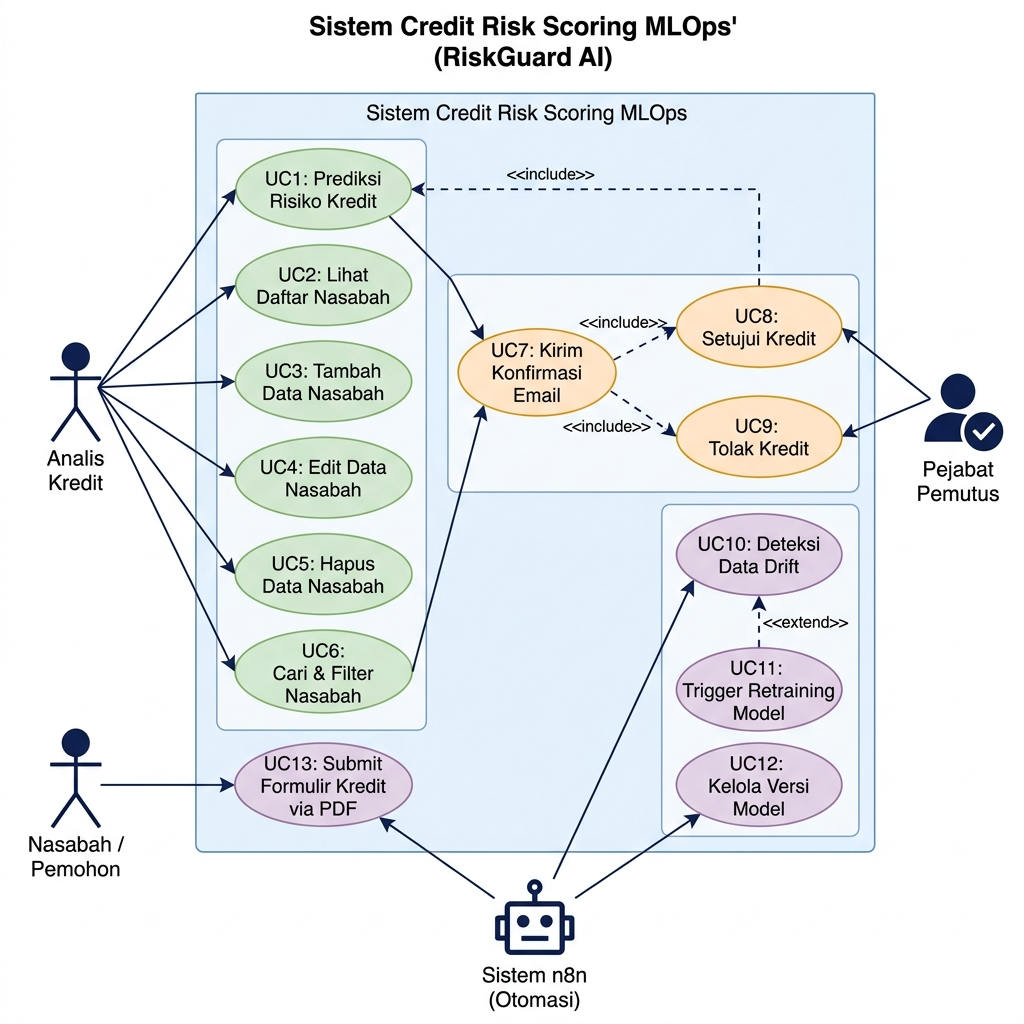
\includegraphics[width=0.92\textwidth]{bab4/use_case_diagram_1783675834026.png}
\caption{Diagram use case keseluruhan sistem credit risk scoring berbasis MLOps}
\label{fig:bab4_use_case_diagram}
\end{figure}

\section{Validasi Awal Dataset Sintetis}
\label{sec:bab4_dataset_sintetis}
Bagian ini menyajikan hasil validasi awal terhadap dataset sintetis yang rancangan pembentukannya telah dijelaskan pada Bab III. Validasi dilakukan untuk memastikan bahwa struktur atribut, format nilai, dan relasi antarkolom pada sampel data tetap konsisten dengan karakteristik umum data kredit konsumtif pada praktik perbankan.

Sebanyak 50 baris sampel data sintetis ditinjau sebagai bagian dari pemeriksaan kewajaran struktur data. Tabel \ref{tab:nasabah_normal} menampilkan 10 baris sampel dari data yang telah ditinjau tersebut. Sampel ini digunakan sebagai bukti bahwa dataset tidak hanya dibangkitkan secara numerik, tetapi juga memiliki atribut identitas, pekerjaan, finansial, histori kredit, parameter risiko, dan indikator makroekonomi yang saling berhubungan secara logis.

\begin{landscape}
\begin{scriptsize}
\setlength{\tabcolsep}{2pt}
\begin{longtable}{p{3.2cm} *{10}{>{\centering\arraybackslash}p{1.1cm}}}
\caption{Profil Data 10 Nasabah Normal}
\label{tab:nasabah_normal} \\
\toprule
\textbf{Fitur / Atribut} & \textbf{Nasabah 1} & \textbf{Nasabah 2} & \textbf{Nasabah 3} & \textbf{Nasabah 4} & \textbf{Nasabah 5} & \textbf{Nasabah 6} & \textbf{Nasabah 7} & \textbf{Nasabah 8} & \textbf{Nasabah 9} & \textbf{Nasabah 10} \\
\midrule
\endfirsthead
\multicolumn{11}{c}{{\tablename\ \thetable{} -- Lanjutan dari halaman sebelumnya}} \\
\toprule
\textbf{Fitur / Atribut} & \textbf{Nasabah 1} & \textbf{Nasabah 2} & \textbf{Nasabah 3} & \textbf{Nasabah 4} & \textbf{Nasabah 5} & \textbf{Nasabah 6} & \textbf{Nasabah 7} & \textbf{Nasabah 8} & \textbf{Nasabah 9} & \textbf{Nasabah 10} \\
\midrule
\endhead
\midrule
\multicolumn{11}{r}{{Bersambung ke halaman berikutnya...}} \\
\endfoot
\bottomrule
\endlastfoot
Customer ID & CUST00001 & CUST00002 & CUST00004 & CUST00007 & CUST00009 & CUST00016 & CUST00019 & CUST00020 & CUST00035 & CUST00036 \\
Nama Nasabah & Gina Pudjiastuti & Violet Utami & Jinawi Prakasa & Padmi Wasita & Ir. Rini Hidayanto & Eman Suartini & Shakila Safitri & Darijan Nababan & Drs. Aurora Pertiwi, S.I.Kom & Wage Najmudin \\
Usia & 64 tahun & 59 tahun & 52 tahun & 63 tahun & 55 tahun & 47 tahun & 46 tahun & 68 tahun & 63 tahun & 56 tahun \\
Jenis Kelamin & Perempuan & Perempuan & Perempuan & Laki-laki & Perempuan & Perempuan & Laki-laki & Perempuan & Perempuan & Laki-laki \\
Status Pernikahan & Menikah & Belum menikah & Menikah & Menikah & Menikah & Cerai & Menikah & Menikah & Cerai & Menikah \\
Jenis Pekerjaan & Pensiunan & Pensiunan & Pensiunan & Pensiunan & Pensiunan & Pensiunan & PNS Purna Bakti & Pensiunan & Pensiunan & Pensiunan \\
Status Pensiun & Pensiun & Pensiun & Pensiun & Pensiun & Aktif & Menjelang pensiun & Menjelang pensiun & Pensiun & Pensiun & Pensiun \\
Pendapatan Bulanan & Rp 3.794.553 & Rp 3.285.278 & Rp 7.896.082 & Rp 837.852 & Rp 2.640.712 & Rp 7.998.989 & Rp 7.068.094 & Rp 6.269.345 & Rp 5.789.716 & Rp 5.299.319 \\
Jumlah Uang Pensiun & Rp 3.035.642 & Rp 2.628.222 & Rp 6.316.866 & Rp 670.282 & Rp 2.112.569 & Rp 6.399.191 & Rp 0 & Rp 5.015.476 & Rp 4.631.773 & Rp 4.239.455 \\
Sumber Gaji & Taspen & Taspen & Kementerian & Kementerian & Taspen & Taspen & Kementerian & Pemerintah Daerah & Kementerian & Kementerian \\
Skor Risiko Pemberi Kerja & 9,72\% & 8,37\% & 9,41\% & 8,70\% & 8,81\% & 11,93\% & 15,67\% & 10,63\% & 10,25\% & 9,35\% \\
Tipe Pemberi Kerja & Government & Government & Swasta & Government & Government & Government & BUMN & BUMN & Government & Government \\
Stabilitas Pendapatan & 50,00\% & 78,17\% & 98,09\% & 95,88\% & 100,00\% & 95,49\% & 70,55\% & 81,02\% & 69,52\% & 64,78\% \\
Rasio Pengeluaran Medis & 42,09\% & 36,60\% & 25,91\% & 40,74\% & 24,38\% & 18,96\% & 16,92\% & 45,00\% & 24,10\% & 31,42\% \\
Volatilitas Gaji & 37,10\% & 20,05\% & 16,83\% & 11,53\% & 10,51\% & 13,87\% & 22,64\% & 19,19\% & 33,76\% & 20,44\% \\
Saldo Rekening Rata-rata & Rp 5.694.253 & Rp 3.940.751 & Rp 8.783.769 & Rp 671.276 & Rp 6.221.424 & Rp 8.226.630 & Rp 17.486.307 & Rp 18.058.906 & Rp 8.497.370 & Rp 10.093.795 \\
Total Cicilan Aktif & 4 & 3 & 3 & 1 & 2 & 3 & 2 & 4 & 3 & 3 \\
Jumlah Pinjaman Lain & 0 & 1 & 2 & 1 & 0 & 1 & 2 & 2 & 0 & 2 \\
Debt-to-Income (DTI) & 60,00\% & 60,00\% & 60,00\% & 60,00\% & 60,00\% & 60,00\% & 60,00\% & 60,00\% & 60,00\% & 60,00\% \\
Skor Kredit Biro (OJK) & 760 & 706 & 615 & 733 & 691 & 704 & 782 & 659 & 755 & 686 \\
Bulan Tunggakan (Past Due) & 0 & 0 & 0 & 0 & 1 & 0 & 0 & 0 & 1 & 2 \\
Lama Riwayat Kredit & 7 tahun & 4 tahun & 5 tahun & 13 tahun & 16 tahun & 5 tahun & 14 tahun & 12 tahun & 8 tahun & 11 tahun \\
Skor Risiko Kesehatan & 0,3954 & 0,6984 & 0,3497 & 0,4720 & 0,3358 & 0,3863 & 0,3126 & 0,4848 & 0,4040 & 0,6703 \\
Memiliki Penyakit Kronis & Tidak & Tidak & Tidak & Ya & Tidak & Ya & Tidak & Tidak & Ya & Tidak \\
Grade Pemeriksaan Medis & Kuning & Hijau & Hijau & Kuning & Hijau & Hijau & Hijau & Hijau & Hijau & Merah \\
Status Asuransi Jiwa & Ada & Ada & Ada & Ada & Ada & Ada & Ada & Ada & Ada & Lapsed \\
Uang Pertanggungan Asuransi & Rp 74.568.148 & Rp 93.427.960 & Rp 160.876.644 & Rp 19.522.187 & Rp 60.489.422 & Rp 106.996.685 & Rp 210.987.989 & Rp 77.736.947 & Rp 111.620.706 & Rp 0 \\
Perusahaan Asuransi & A & N/A & N/A & C & N/A & A & B & B & N/A & A \\
Premi Asuransi Bulanan & Rp 41.236 & Rp 37.399 & Rp 322.020 & Rp 19.283 & Rp 90.346 & Rp 309.770 & Rp 127.723 & Rp 234.098 & Rp 68.648 & Rp 0 \\
Loan ID & LOAN00001 & LOAN00002 & LOAN00004 & LOAN00007 & LOAN00009 & LOAN00016 & LOAN00019 & LOAN00020 & LOAN00035 & LOAN00036 \\
Jenis Produk Kredit & Kredit Pensiun & KTA & Vehicle Loan & KTA & Kredit Pensiun & Vehicle Loan & KTA & Vehicle Loan & Payroll loan & Kredit Pensiun \\
Tanggal Pencairan & 2024-07-07 & 2024-08-29 & 2024-10-19 & 2024-12-25 & 2024-05-18 & 2024-07-12 & 2024-06-29 & 2024-10-24 & 2024-07-02 & 2024-04-19 \\
Jumlah Pinjaman & Rp 445.817.427 & Rp 91.001.085 & Rp 259.288.337 & Rp 133.424.947 & Rp 229.291.603 & Rp 378.063.313 & Rp 352.642.843 & Rp 81.310.033 & Rp 281.474.657 & Rp 393.324.410 \\
Tenor (Bulan) & 36 bulan & 24 bulan & 36 bulan & 24 bulan & 60 bulan & 60 bulan & 36 bulan & 12 bulan & 36 bulan & 60 bulan \\
Suku Bunga & 10,26\% & 7,05\% & 7,29\% & 6,19\% & 7,67\% & 11,50\% & 6,81\% & 8,74\% & 6,22\% & 11,79\% \\
Memiliki Agunan & Tidak & Tidak & Ya & Tidak & Tidak & Ya & Tidak & Ya & Tidak & Tidak \\
Loan-to-Value (LTV) & 0,00\% & 0,00\% & 73,78\% & 0,00\% & 0,00\% & 64,68\% & 0,00\% & 81,00\% & 0,00\% & 0,00\% \\
Sisa Pinjaman (Outstanding) & Rp 339.481.396 & Rp 51.108.601 & Rp 210.129.567 & Rp 80.717.080 & Rp 211.496.051 & Rp 311.998.546 & Rp 217.816.877 & Rp 40.116.401 & Rp 257.162.920 & Rp 224.891.067 \\
Penarikan Tunai Terakhir & Rp 1.689.874 & Rp 1.593.090 & Rp 2.431.573 & Rp 107.371 & Rp 329.034 & Rp 3.057.805 & Rp 1.558.622 & Rp 1.474.772 & Rp 619.314 & Rp 2.179.738 \\
Frekuensi Transaksi Digital & 6 & 4 & 2 & 5 & 4 & 8 & 6 & 6 & 6 & 2 \\
Pengeluaran Kartu & Rp 2.344.281 & Rp 1.305.067 & Rp 5.289.440 & Rp 516.051 & Rp 653.734 & Rp 4.066.357 & Rp 3.243.903 & Rp 4.285.389 & Rp 3.809.882 & Rp 2.027.416 \\
Probability of Default (PD) & 17,80\% & 33,58\% & 44,18\% & 22,13\% & 49,17\% & 60,25\% & 12,13\% & 41,57\% & 72,54\% & 95,22\% \\
Flag Gagal Bayar & 0 (Normal) & 0 (Normal) & 0 (Normal) & 0 (Normal) & 0 (Normal) & 0 (Normal) & 0 (Normal) & 0 (Normal) & 0 (Normal) & 0 (Normal) \\
Loss Given Default (LGD) & 35,53\% & 40,37\% & 26,14\% & 43,17\% & 41,50\% & 25,31\% & 37,87\% & 28,95\% & 31,98\% & 54,85\% \\
Exposure at Default (EAD) & Rp 335.521.586 & Rp 46.974.181 & Rp 206.268.544 & Rp 78.150.696 & Rp 193.322.196 & Rp 282.194.173 & Rp 211.283.836 & Rp 38.057.267 & Rp 236.291.708 & Rp 209.726.895 \\
Expected Loss (EL) & Rp 21.228.120 & Rp 6.368.037 & Rp 23.822.213 & Rp 7.467.822 & Rp 39.453.423 & Rp 43.035.391 & Rp 9.705.088 & Rp 4.579.550 & Rp 54.818.226 & Rp 109.536.605 \\

\end{longtable}
\end{scriptsize}
\end{landscape}

Berdasarkan sampel tersebut, dataset sintetis dinilai memadai untuk digunakan pada tahap pengujian berikutnya karena telah memuat variasi atribut nasabah, produk kredit, indikator risiko, serta variabel makroekonomi yang dibutuhkan dalam proses \textit{credit risk scoring}. Dengan demikian, pengujian pada bagian selanjutnya dapat difokuskan pada kualitas preprocessing, performa model, validasi quality gate, dan kesiapan implementasi MLOps.


\section{Pengujian Preprocessing WoE dan IV}
\label{sec:bab4_preprocessing_woe_iv}
Tahap preprocessing menggunakan \textit{Weight of Evidence} (WoE) untuk mengubah fitur numerik dan kategorikal menjadi representasi yang berkaitan dengan \textit{log-odds} gagal bayar. Sementara itu, \textit{Information Value} (IV) digunakan untuk menilai kekuatan prediktif setiap fitur terhadap target \textit{missed\_payment\_flag}. Kombinasi WoE dan IV dipilih karena umum digunakan pada \textit{credit scoring}, mudah dijelaskan, dan dapat membantu membedakan fitur yang informatif dari fitur yang bersifat noise.

Hasil perhitungan IV menunjukkan bahwa fitur \textit{bureau\_score} menjadi prediktor terkuat dengan nilai IV sebesar 0,408071. Fitur ini dikategorikan sebagai \textit{strong predictor}, sehingga dipertahankan sebagai masukan penting bagi model. Beberapa fitur lain seperti \textit{past\_due\_months}, \textit{marital\_status}, \textit{term\_months}, \textit{age}, \textit{life\_insurance\_coverage}, \textit{insurance\_premium\_monthly}, dan \textit{insurance\_status} berada pada kategori \textit{medium predictor}. Fitur dengan nilai IV di bawah 0,02, seperti \textit{credit\_history\_length}, \textit{avg\_account\_balance}, \textit{digital\_payment\_frequency}, dan beberapa fitur makroekonomi, dieliminasi karena kontribusi prediktifnya sangat rendah.

\begin{table}[H]
\centering
\caption{Ringkasan fitur utama berdasarkan nilai Information Value}
\label{tab:bab4_iv_summary}
\begin{tabular}{|p{0.06\textwidth}|p{0.32\textwidth}|p{0.17\textwidth}|p{0.27\textwidth}|}
\hline
\textbf{No.} & \textbf{Fitur} & \textbf{Nilai IV} & \textbf{Interpretasi} \\
\hline
1 & \textit{bureau\_score} & 0,408071 & \textit{Strong predictor} \\
\hline
2 & \textit{past\_due\_months} & 0,215358 & \textit{Medium predictor} \\
\hline
3 & \textit{marital\_status} & 0,164296 & \textit{Medium predictor} \\
\hline
4 & \textit{term\_months} & 0,154057 & \textit{Medium predictor} \\
\hline
6 & \textit{life\_insurance\_coverage} & 0,112946 & \textit{Medium predictor} \\
\hline
7 & \textit{insurance\_premium\_monthly} & 0,112611 & \textit{Medium predictor} \\
\hline
8 & \textit{insurance\_status} & 0,105535 & \textit{Medium predictor} \\
\hline
\end{tabular}
\end{table}

\begin{figure}[H]
\centering
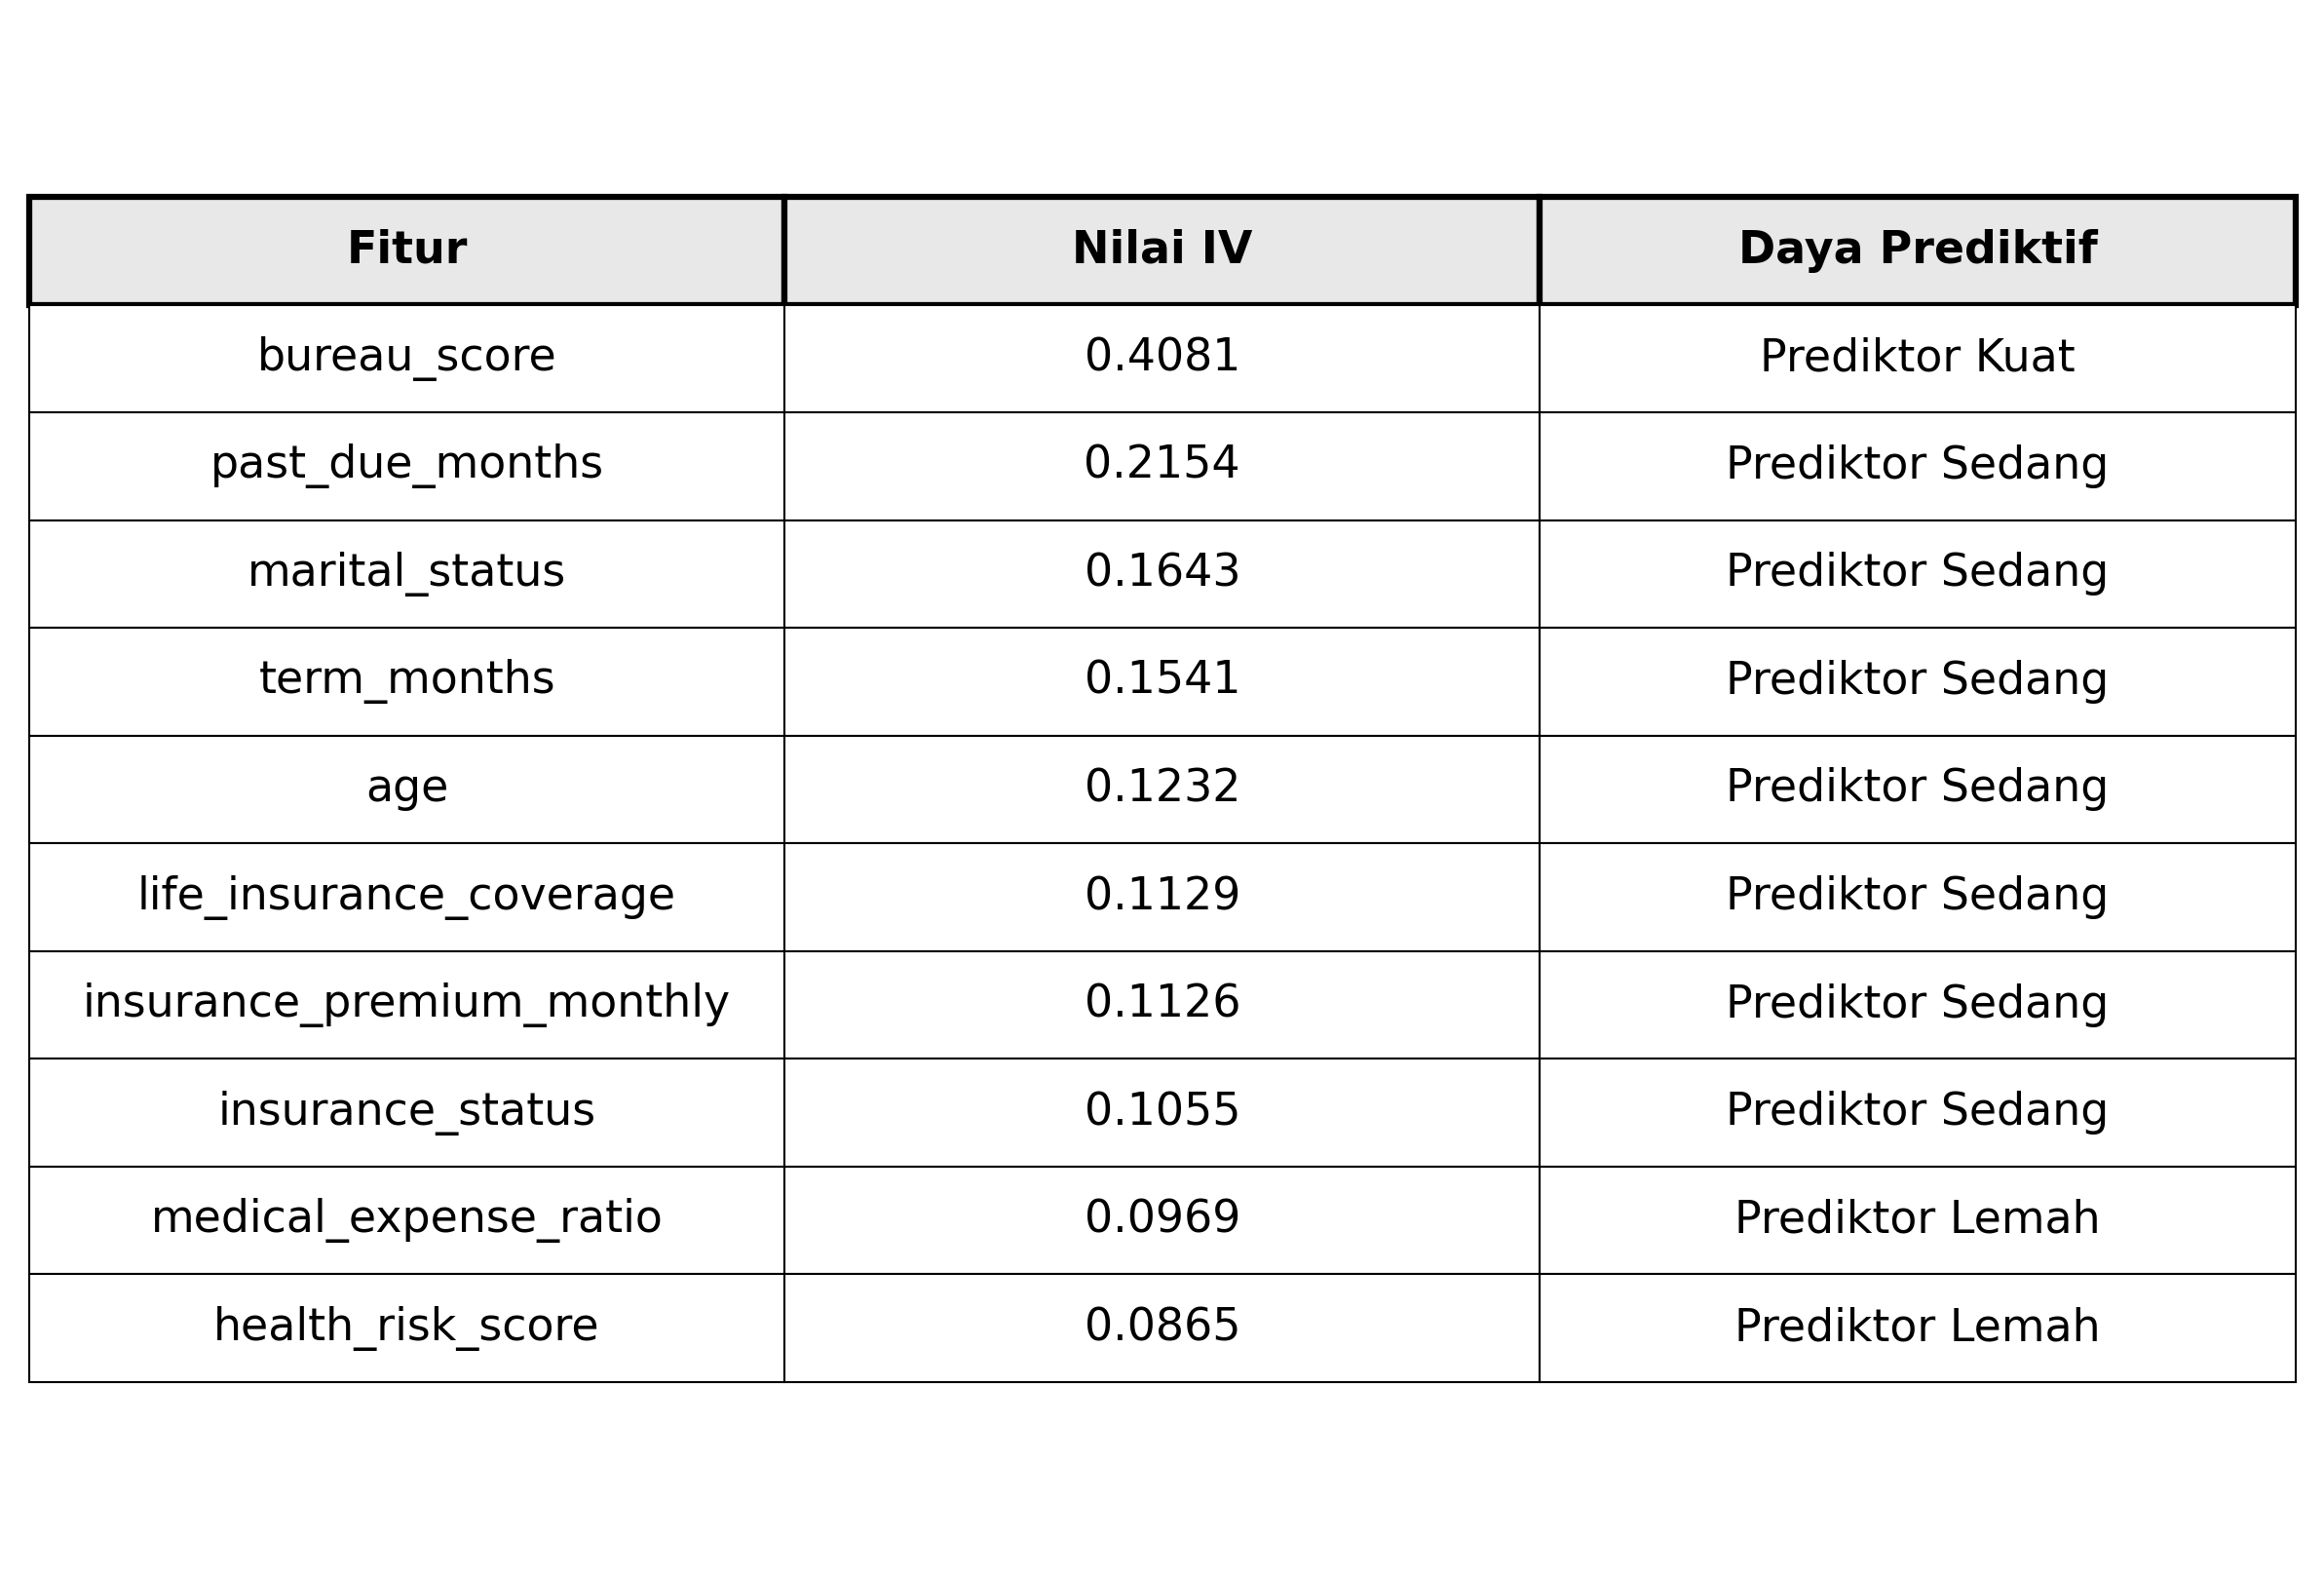
\includegraphics[width=0.9\textwidth]{bab4/Tabel_IV_Format.png}
\caption{Tabel nilai Information Value untuk seleksi fitur}
\label{fig:bab4_tabel_iv}
\end{figure}



Selain nilai IV, hasil binning WoE digunakan untuk melihat pola hubungan antara kelompok nilai fitur dan risiko gagal bayar. Gambar \ref{fig:bab4_woe_binning} menunjukkan bahwa setiap bin memiliki nilai WoE yang dapat dibandingkan, sehingga perubahan tingkat risiko pada masing-masing kelompok fitur dapat dianalisis secara lebih terstruktur.

\begin{figure}[H]
\centering
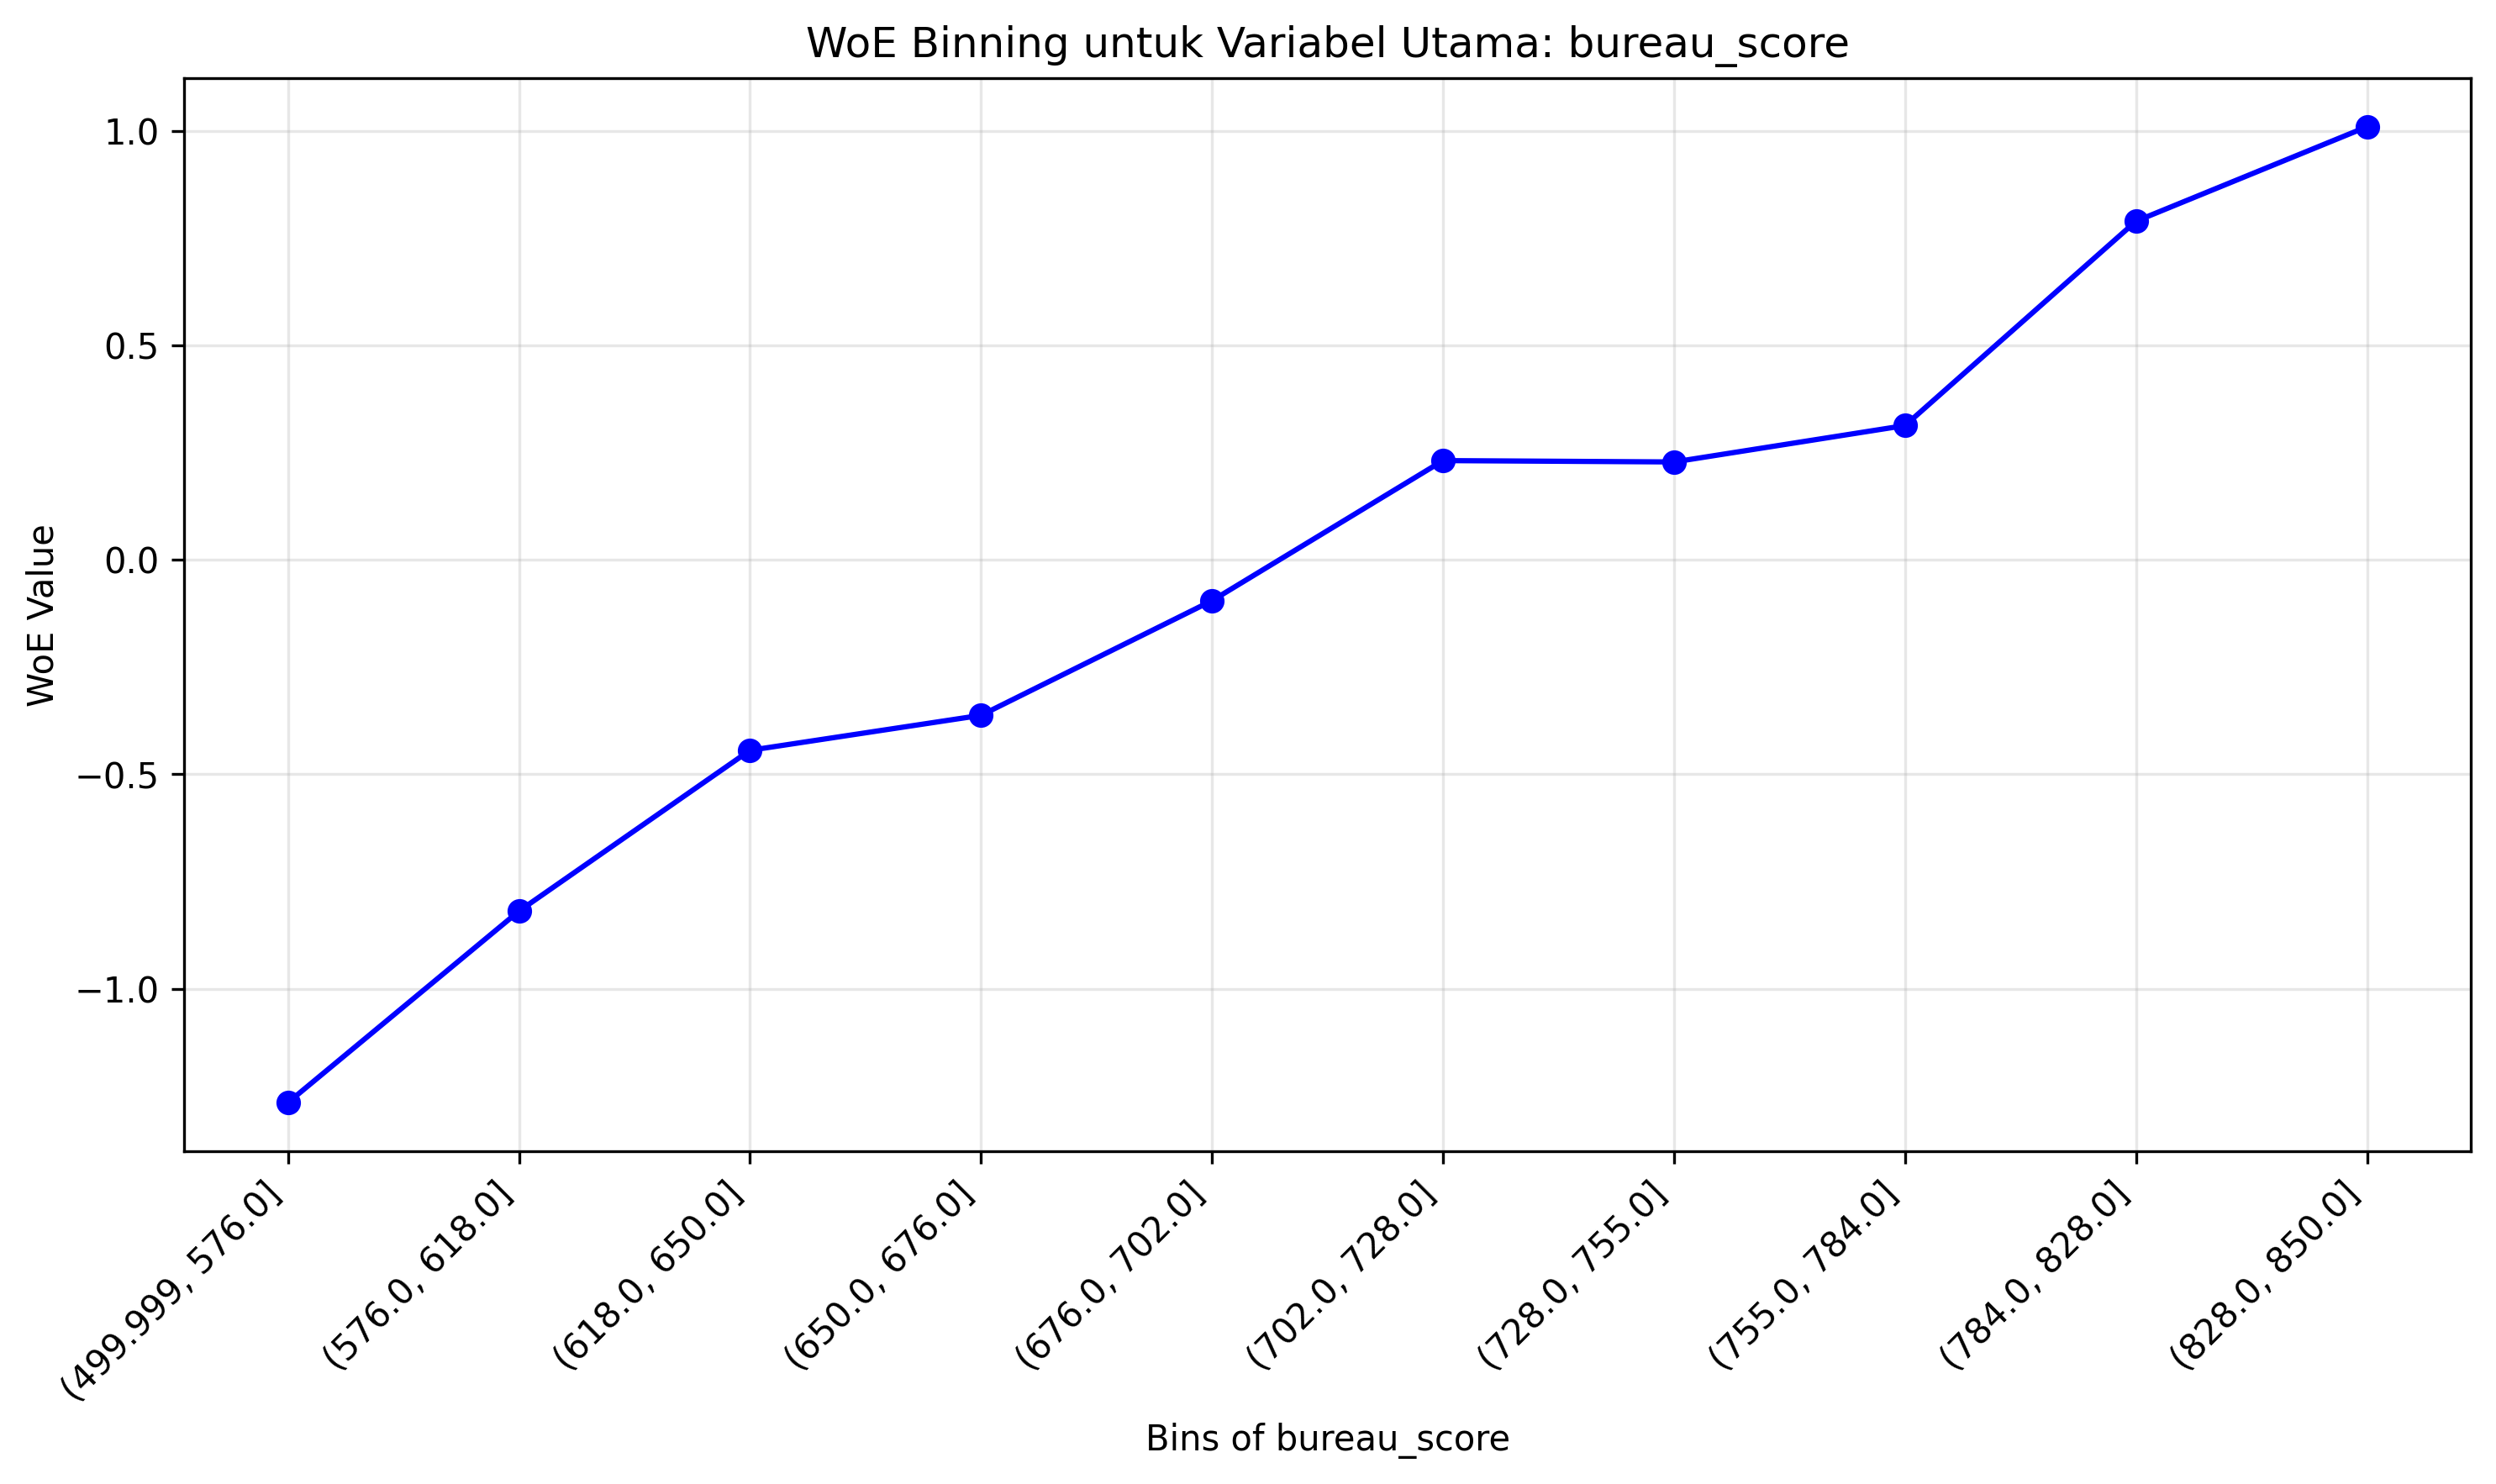
\includegraphics[width=0.86\textwidth]{bab4/WoE_Binning_plot.png}
\caption{Visualisasi WoE binning pada fitur utama}
\label{fig:bab4_woe_binning}
\end{figure}

\section{Pengujian Penanganan Ketidakseimbangan Kelas}
\label{sec:bab4_smote}
Dataset risiko kredit memiliki karakteristik kelas yang tidak seimbang karena jumlah nasabah yang tidak mengalami gagal bayar lebih besar dibandingkan jumlah nasabah yang mengalami gagal bayar. Pada data awal, kelas non-default berjumlah 8.520 nasabah atau 85,2\%, sedangkan kelas default berjumlah 1.480 nasabah atau 14,8\%. Ketimpangan ini berpotensi membuat model cenderung memprediksi kelas mayoritas dan mengabaikan pola pada kelas default.

Untuk mengatasi masalah tersebut, SMOTE diterapkan pada data latih setelah proses pembagian dataset. Penerapan SMOTE hanya dilakukan pada data latih agar tidak terjadi kebocoran informasi ke data validasi maupun data uji. Hasilnya, jumlah data default pada data latih meningkat sehingga distribusi kelas menjadi seimbang.

\begin{table}[H]
\centering
\caption{Distribusi kelas sebelum dan sesudah SMOTE pada data latih}
\label{tab:bab4_smote}
\begin{tabular}{|p{0.25\textwidth}|p{0.18\textwidth}|p{0.18\textwidth}|p{0.17\textwidth}|p{0.14\textwidth}|}
\hline
\textbf{Kondisi} & \textbf{Non-Default} & \textbf{Default} & \textbf{Total} & \textbf{Rasio} \\
\hline
Sebelum SMOTE & 5.964 & 1.036 & 7.000 & 85,2\% : 14,8\% \\
\hline
Setelah SMOTE & 5.964 & 5.964 & 11.928 & 50,0\% : 50,0\% \\
\hline
\end{tabular}
\end{table}

Hasil ini menunjukkan bahwa proses resampling berhasil menyeimbangkan distribusi kelas pada data latih. Dengan distribusi yang lebih seimbang, proses pembelajaran XGBoost memperoleh sinyal yang lebih proporsional dari kedua kelas, khususnya kelas default yang menjadi fokus utama dalam konteks manajemen risiko kredit.

\section{Pengembangan dan Evaluasi Model}
\label{sec:bab4_pemodelan}
Model utama yang digunakan dalam penelitian ini adalah XGBoost. Pemilihan XGBoost didasarkan pada kemampuannya dalam menangani data tabular, memodelkan interaksi antarfitur secara nonlinier, serta menyediakan mekanisme pengendalian kompleksitas model. Pada tahap pelatihan, data hasil transformasi WoE digunakan sebagai masukan model, sedangkan konfigurasi model dipilih melalui \textit{RandomizedSearchCV} dengan 10 iterasi dan 3-Fold Cross Validation.

Parameter yang diuji meliputi \textit{max\_depth}, \textit{learning\_rate}, \textit{n\_estimators}, \textit{subsample}, dan \textit{colsample\_bytree}. Hasil tuning menunjukkan bahwa konfigurasi terbaik diperoleh pada kedalaman pohon 5, \textit{learning rate} 0,01, jumlah estimator 100, \textit{subsample} 0,8, dan \textit{colsample} 0,8, dengan rata-rata AUC validasi sebesar 0,819303.

\begin{table}[H]
\centering
\caption{Ringkasan hasil hyperparameter tuning XGBoost}
\label{tab:bab4_tuning_summary}
\begin{tabular}{|p{0.12\textwidth}|p{0.14\textwidth}|p{0.16\textwidth}|p{0.16\textwidth}|p{0.14\textwidth}|p{0.16\textwidth}|}
\hline
\textbf{Peringkat} & \textbf{Max Depth} & \textbf{Learning Rate} & \textbf{N Estimators} & \textbf{Subsample} & \textbf{Mean AUC} \\
\hline
1 & 5 & 0,01 & 100 & 0,8 & 0,819303 \\
\hline
2 & 5 & 0,05 & 200 & 0,8 & 0,818365 \\
\hline
3 & 5 & 0,10 & 100 & 0,8 & 0,815952 \\
\hline
4 & 3 & 0,10 & 200 & 0,8 & 0,808289 \\
\hline
5 & 3 & 0,01 & 100 & 0,8 & 0,799574 \\
\hline
\end{tabular}
\end{table}

Visualisasi konfigurasi tuning terbaik ditampilkan pada Gambar \ref{fig:bab4_tabel_tuning}. Dokumentasi parameter ini penting agar proses pelatihan model dapat ditelusuri kembali dan direplikasi.

\begin{figure}[H]
\centering
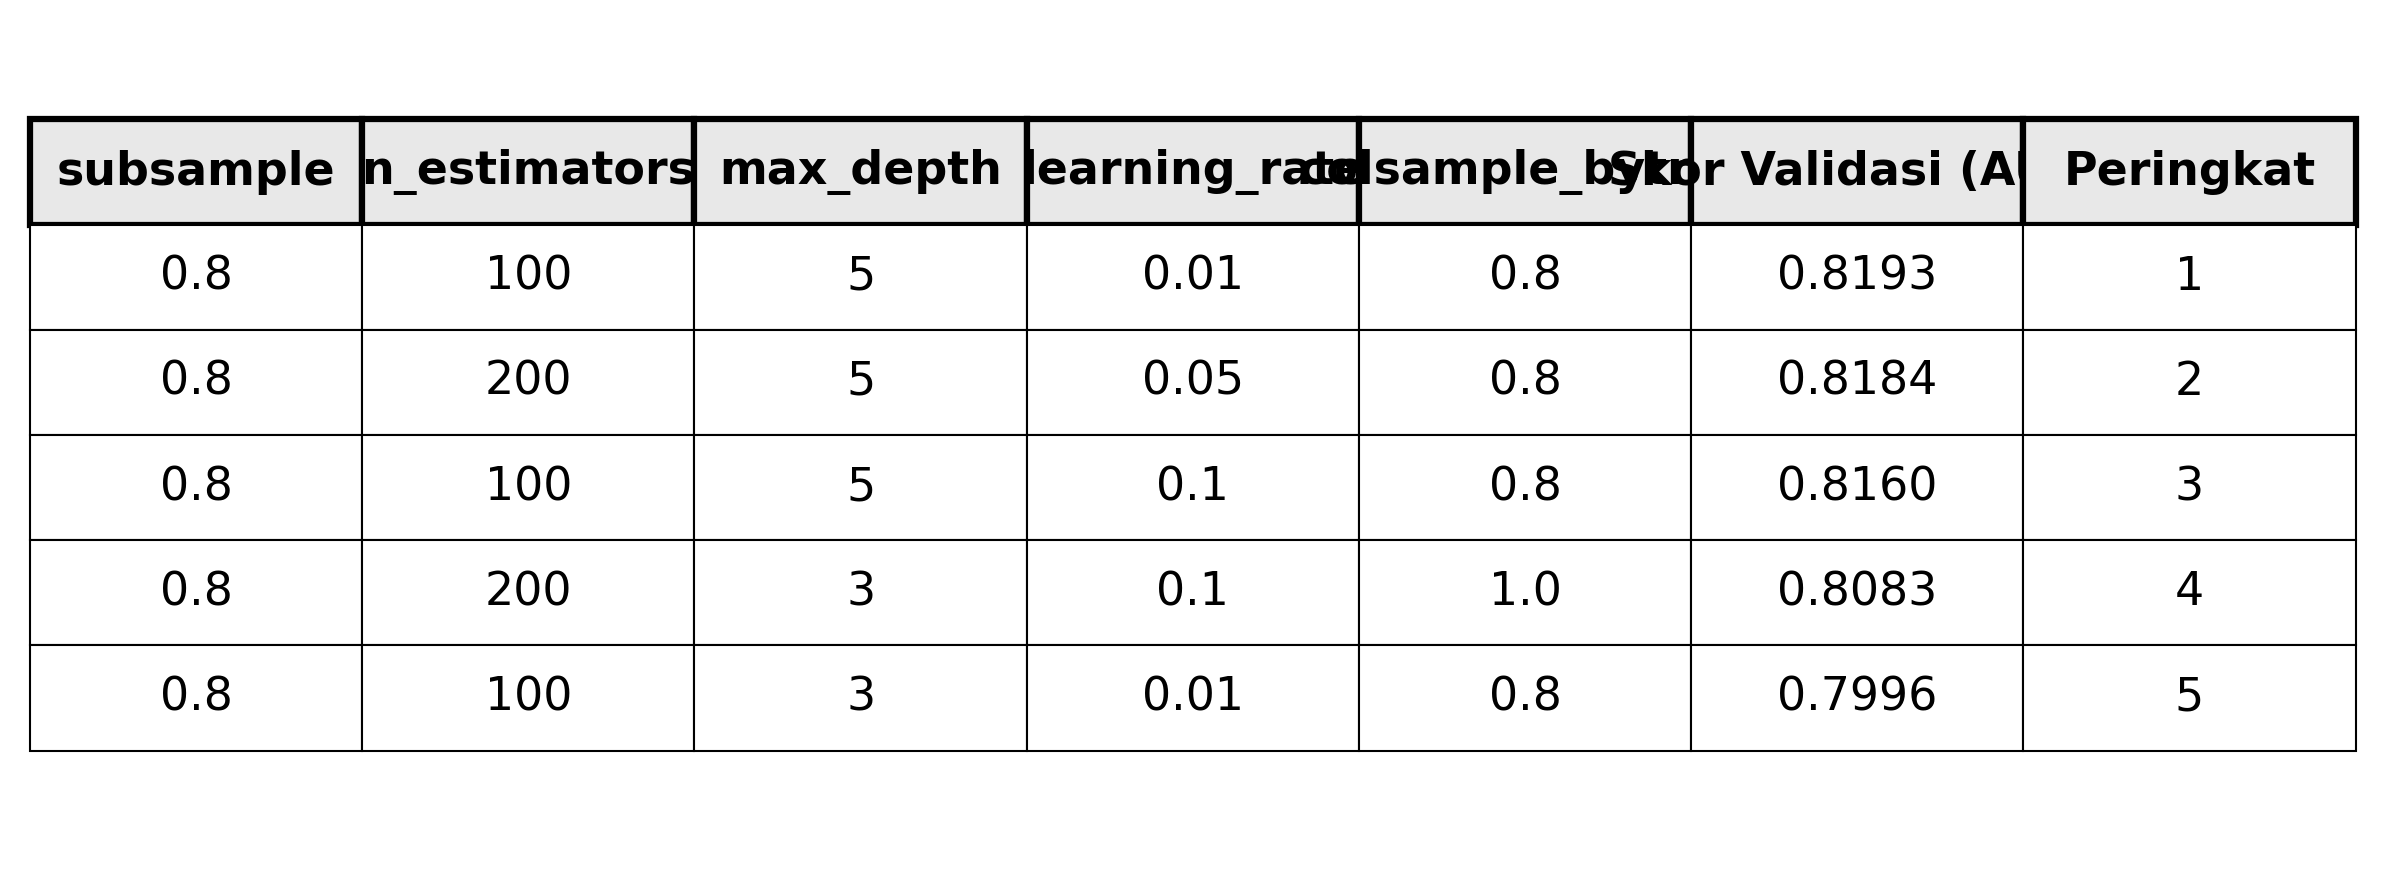
\includegraphics[width=0.86\textwidth]{bab4/Tabel_Tuning_Format.png}
\caption{Konfigurasi hyperparameter terbaik pada model XGBoost}
\label{fig:bab4_tabel_tuning}
\end{figure}

Model terbaik kemudian dievaluasi pada data uji independen. Hasil evaluasi menunjukkan AUC sebesar 0,8262, presisi sebesar 0,8024, recall sebesar 0,7549, dan F1-score sebesar 0,7779. Nilai AUC yang berada di atas 0,80 menunjukkan bahwa model memiliki kemampuan diskriminasi yang baik dalam membedakan nasabah berisiko rendah dan nasabah berisiko tinggi.

Selain metrik evaluasi akhir, proses pelatihan dan pencatatan eksperimen juga diverifikasi melalui antarmuka MLflow. Gambar \ref{fig:bab4_mlflow_experiments} menunjukkan daftar eksperimen \textit{Credit Risk MLOPS} yang tersimpan pada MLflow. Setiap eksperimen merepresentasikan proses pelatihan yang dicatat beserta waktu pembuatan dan pembaruannya, sehingga riwayat eksperimen dapat ditelusuri kembali ketika model perlu dibandingkan atau direproduksi.

\begin{figure}[H]
\centering
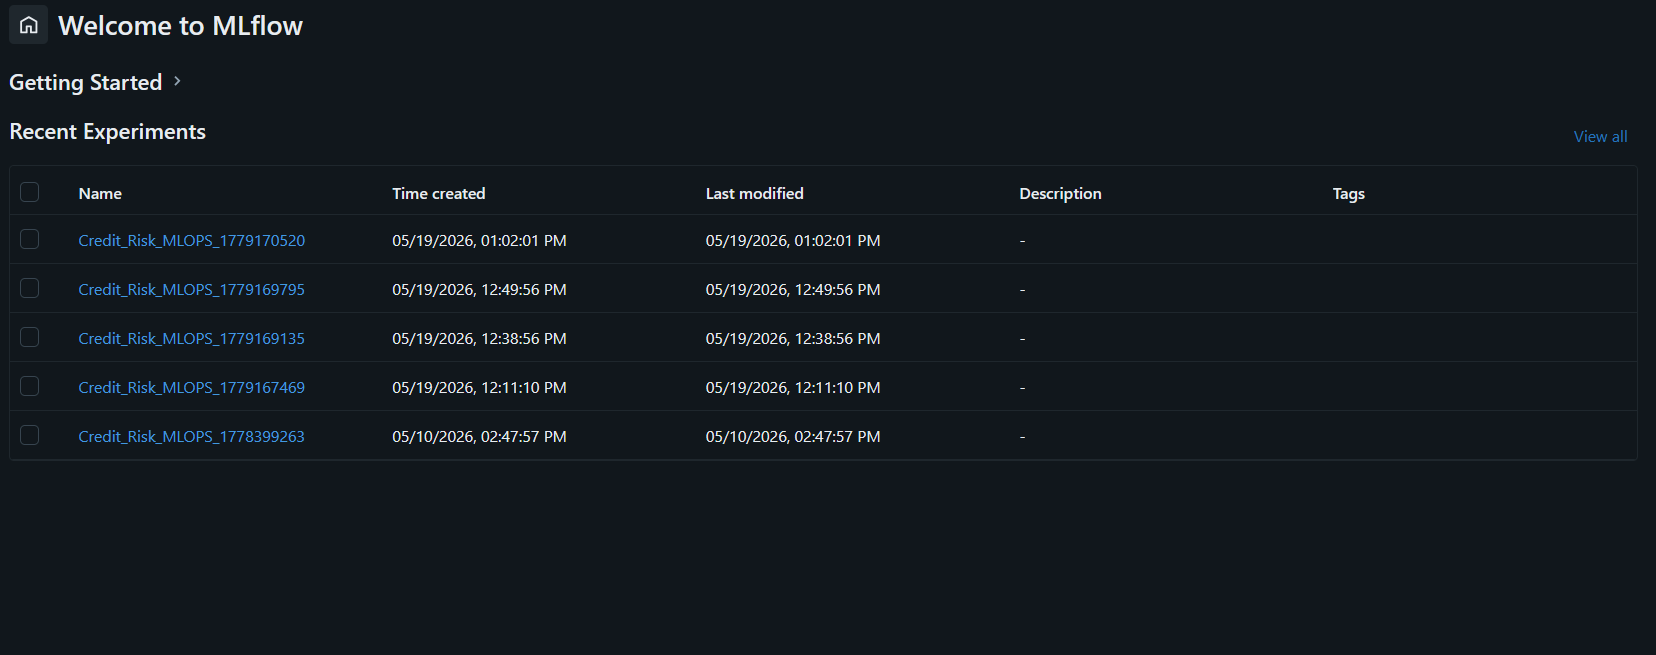
\includegraphics[width=0.92\textwidth]{bab4/Screenshot 2026-05-25 190337.png}
\caption{Daftar eksperimen pelatihan model pada antarmuka MLflow}
\label{fig:bab4_mlflow_experiments}
\end{figure}

\begin{table}[H]
\centering
\caption{Metrik evaluasi model XGBoost pada data uji}
\label{tab:bab4_metrik_model}
\begin{tabular}{|l|c|p{0.45\textwidth}|}
\hline
\textbf{Metrik} & \textbf{Nilai} & \textbf{Interpretasi} \\
\hline
AUC & 0,8262 & Kemampuan diskriminasi model tergolong baik. \\
\hline
Precision & 0,8024 & Sebagian besar prediksi berisiko benar-benar relevan. \\
\hline
Recall & 0,7549 & Model mampu menangkap sebagian besar kasus default. \\
\hline
F1-score & 0,7779 & Keseimbangan presisi dan recall cukup baik. \\
\hline
\end{tabular}
\end{table}

Ringkasan metrik evaluasi juga disajikan pada Gambar \ref{fig:bab4_tabel_metrik}, sedangkan kurva ROC ditunjukkan pada Gambar \ref{fig:bab4_roc_curve}. Kurva ROC digunakan untuk melihat performa model pada berbagai ambang keputusan, bukan hanya pada satu nilai ambang tertentu.

\begin{figure}[H]
\centering
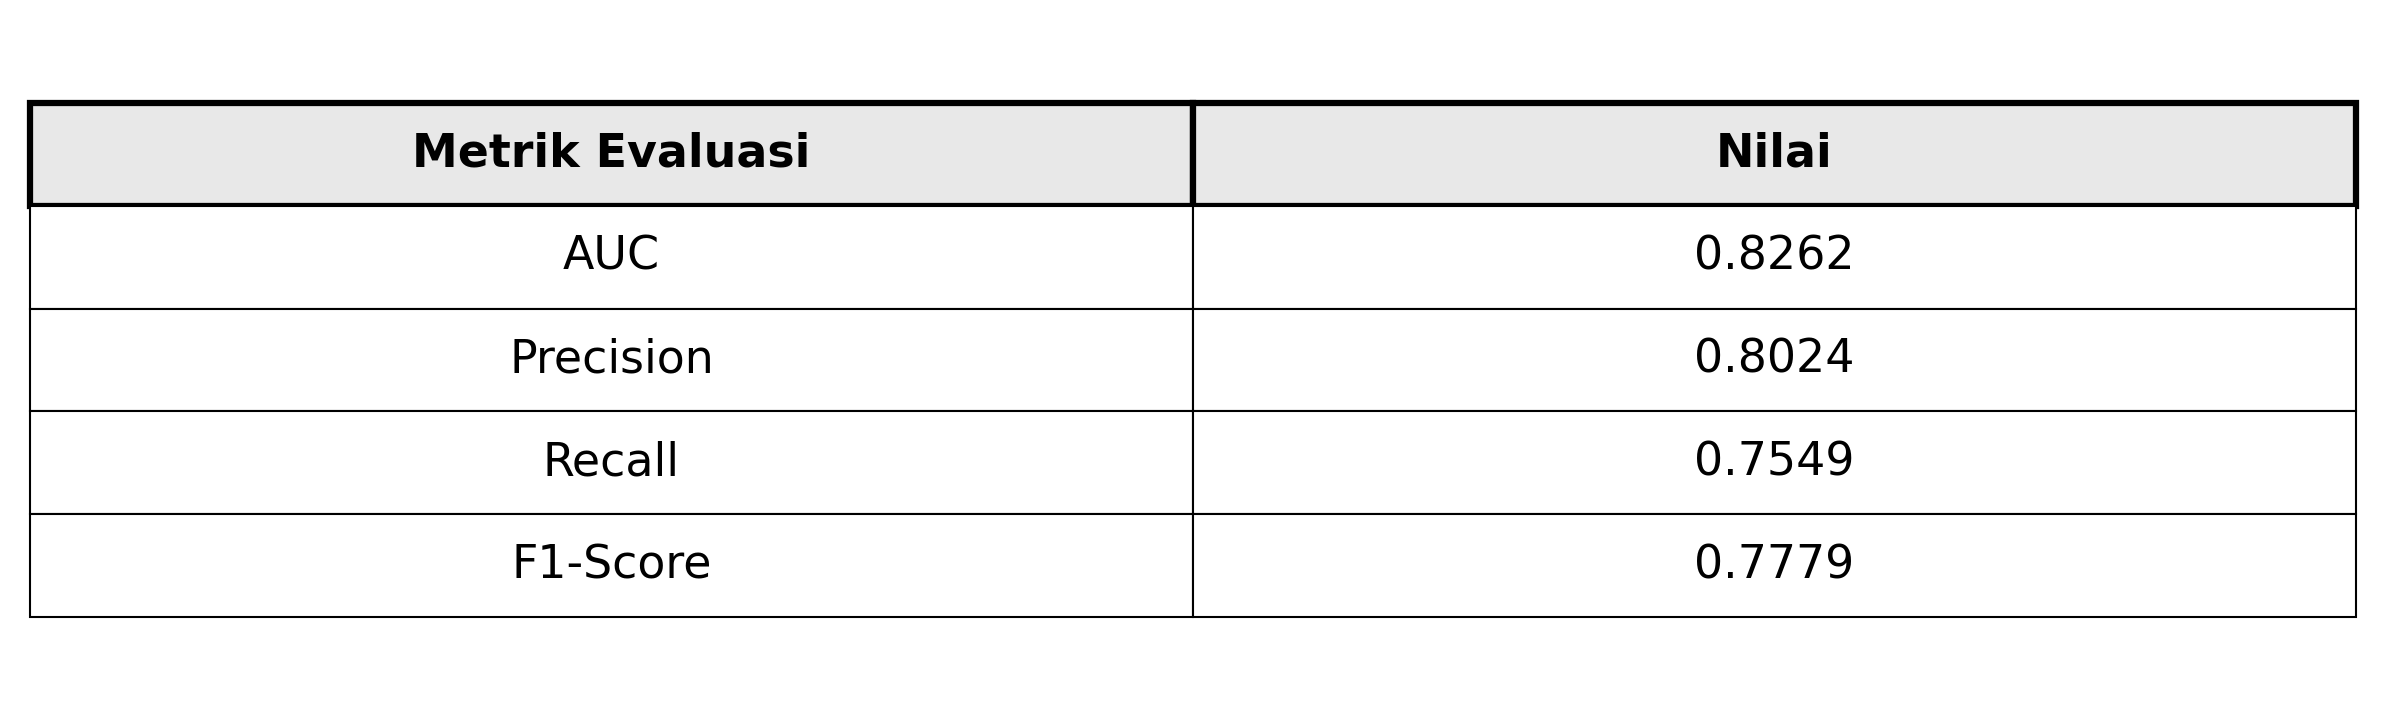
\includegraphics[width=0.86\textwidth]{bab4/Tabel_Metrik_Evaluasi_Format.png}
\caption{Tabel metrik evaluasi model prediktif risiko kredit}
\label{fig:bab4_tabel_metrik}
\end{figure}

\begin{figure}[H]
\centering
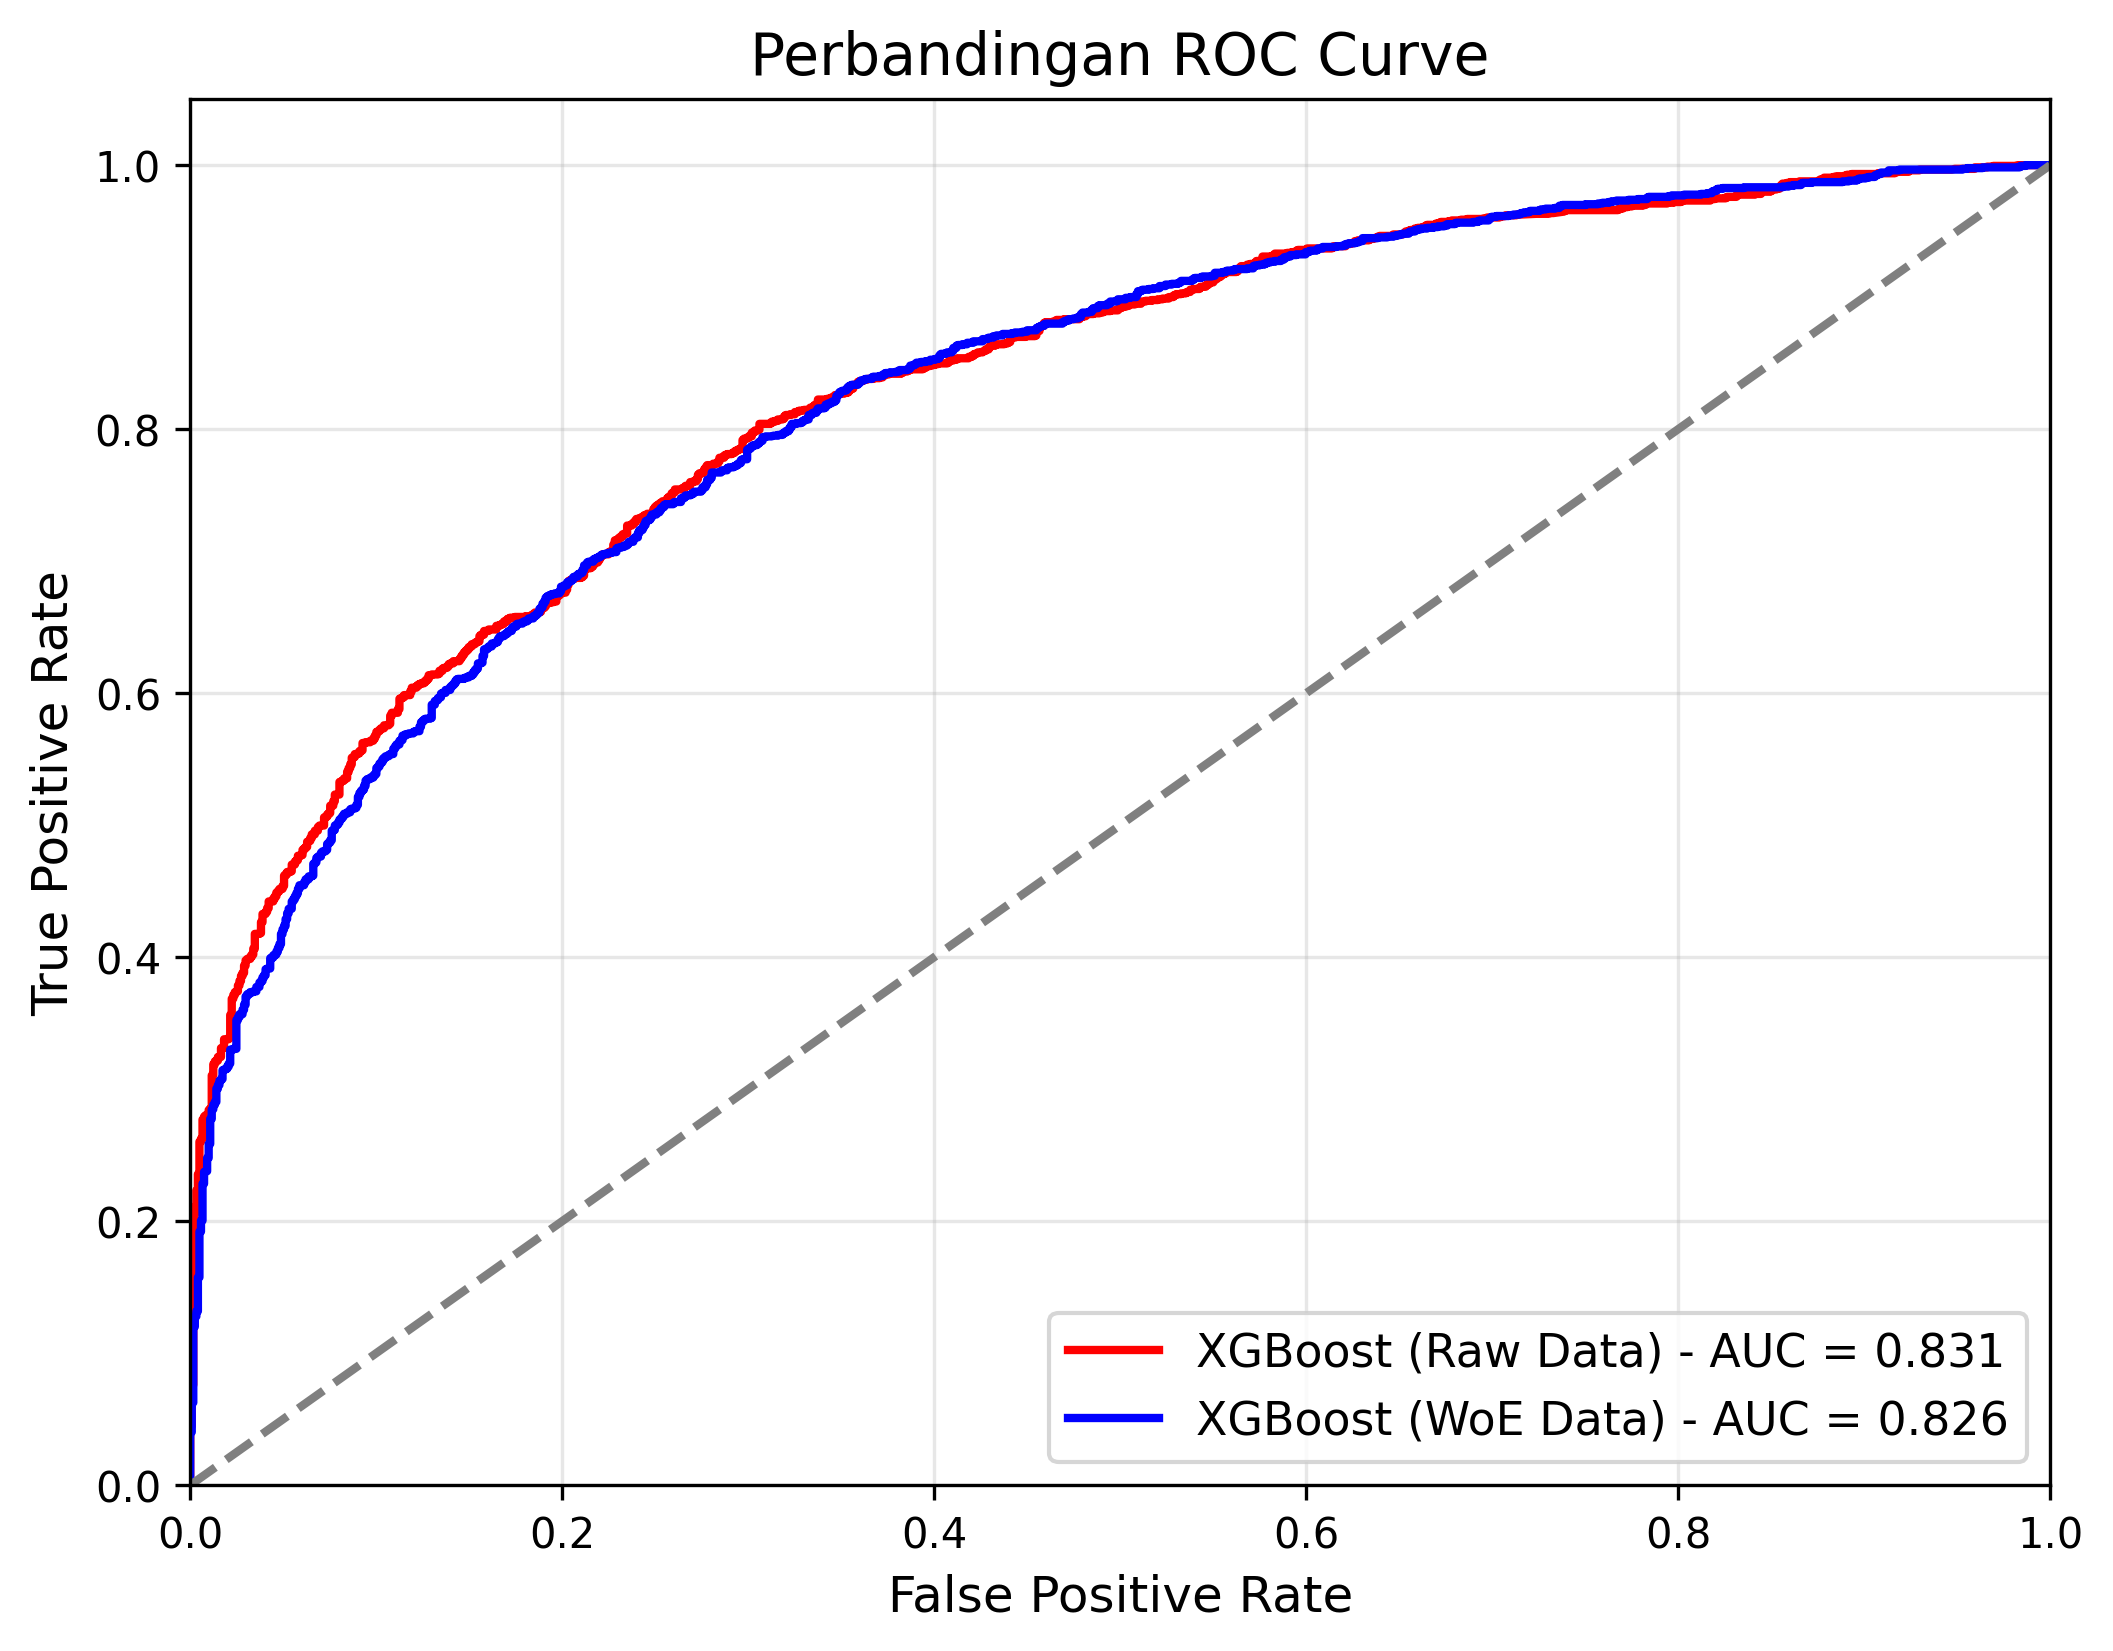
\includegraphics[width=0.8\textwidth]{bab4/ROC_Curve.png}
\caption{Kurva ROC model XGBoost terbaik pada data uji}
\label{fig:bab4_roc_curve}
\end{figure}

Gambar \ref{fig:bab4_confusion_matrix} menunjukkan distribusi prediksi benar dan salah. Matriks ini penting untuk melihat apakah model lebih sering menghasilkan \textit{false positive} atau \textit{false negative}. Dalam konteks kredit, \textit{false negative} perlu diperhatikan karena berarti nasabah berisiko tinggi diklasifikasikan sebagai layak.

\begin{figure}[H]
\centering
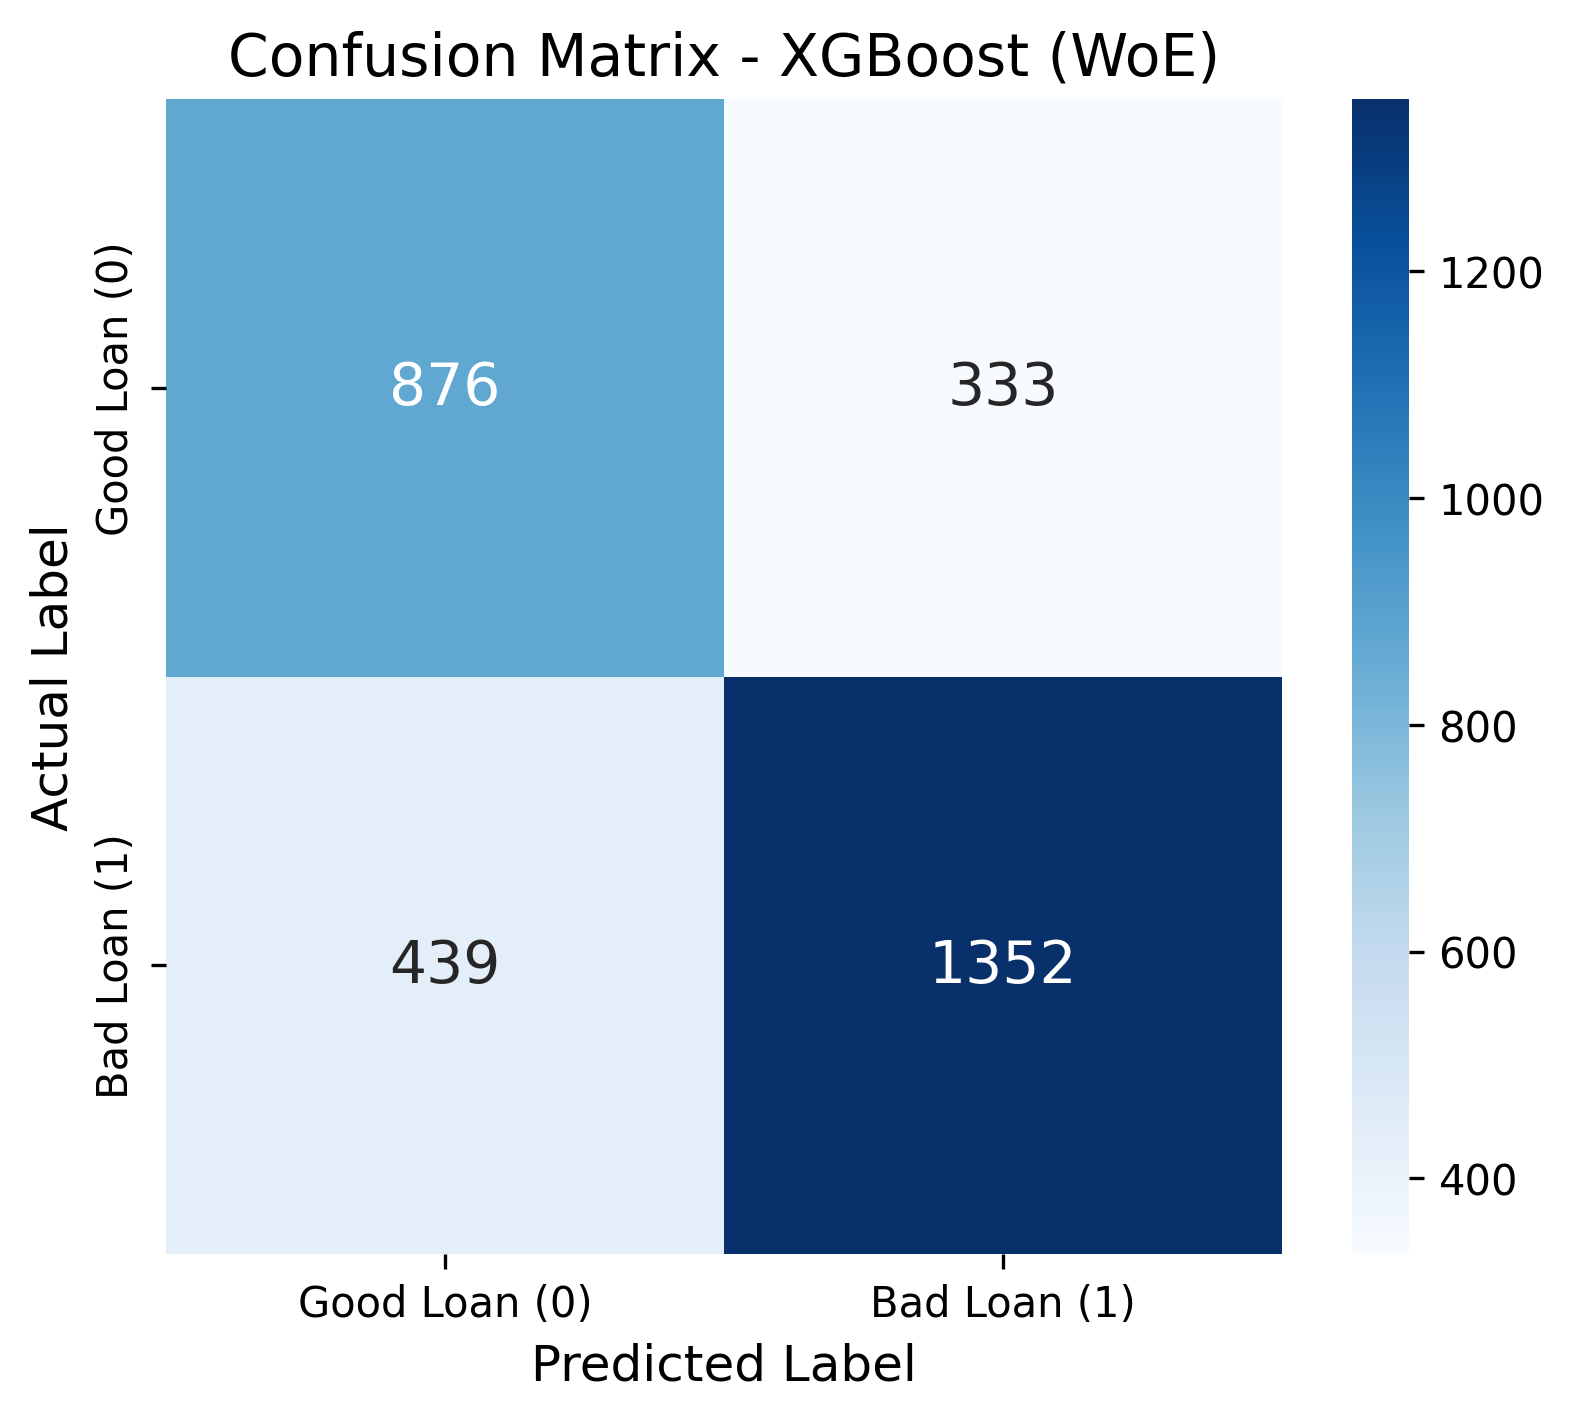
\includegraphics[width=0.62\textwidth]{bab4/Confusion_Matrix.png}
\caption{Confusion matrix hasil pengujian model klasifikasi risiko kredit}
\label{fig:bab4_confusion_matrix}
\end{figure}

Untuk menjelaskan keputusan model, penelitian ini menggunakan SHAP. Gambar \ref{fig:bab4_shap_summary} menunjukkan kontribusi fitur secara global terhadap prediksi model. Berdasarkan visualisasi tersebut, \textit{bureau\_score} menjadi salah satu fitur paling dominan. Skor biro kredit yang rendah cenderung meningkatkan probabilitas default, sedangkan skor yang tinggi cenderung menurunkan risiko. Hal ini sejalan dengan prinsip penilaian kredit, yaitu riwayat kredit menjadi indikator penting dalam menentukan kelayakan nasabah.

\begin{figure}[H]
\centering
\includegraphics[width=0.78\textwidth]{bab4/SHAP_Summary.png}
\caption{SHAP summary plot untuk interpretasi global model XGBoost}
\label{fig:bab4_shap_summary}
\end{figure}

Gambar \ref{fig:bab4_shap_summary_detail} menyajikan ringkasan kontribusi fitur dalam format lain. Visualisasi tambahan ini memperkuat analisis bahwa evaluasi model tidak hanya dilakukan melalui metrik numerik, tetapi juga melalui penjelasan faktor yang memengaruhi prediksi.

\begin{figure}[H]
\centering
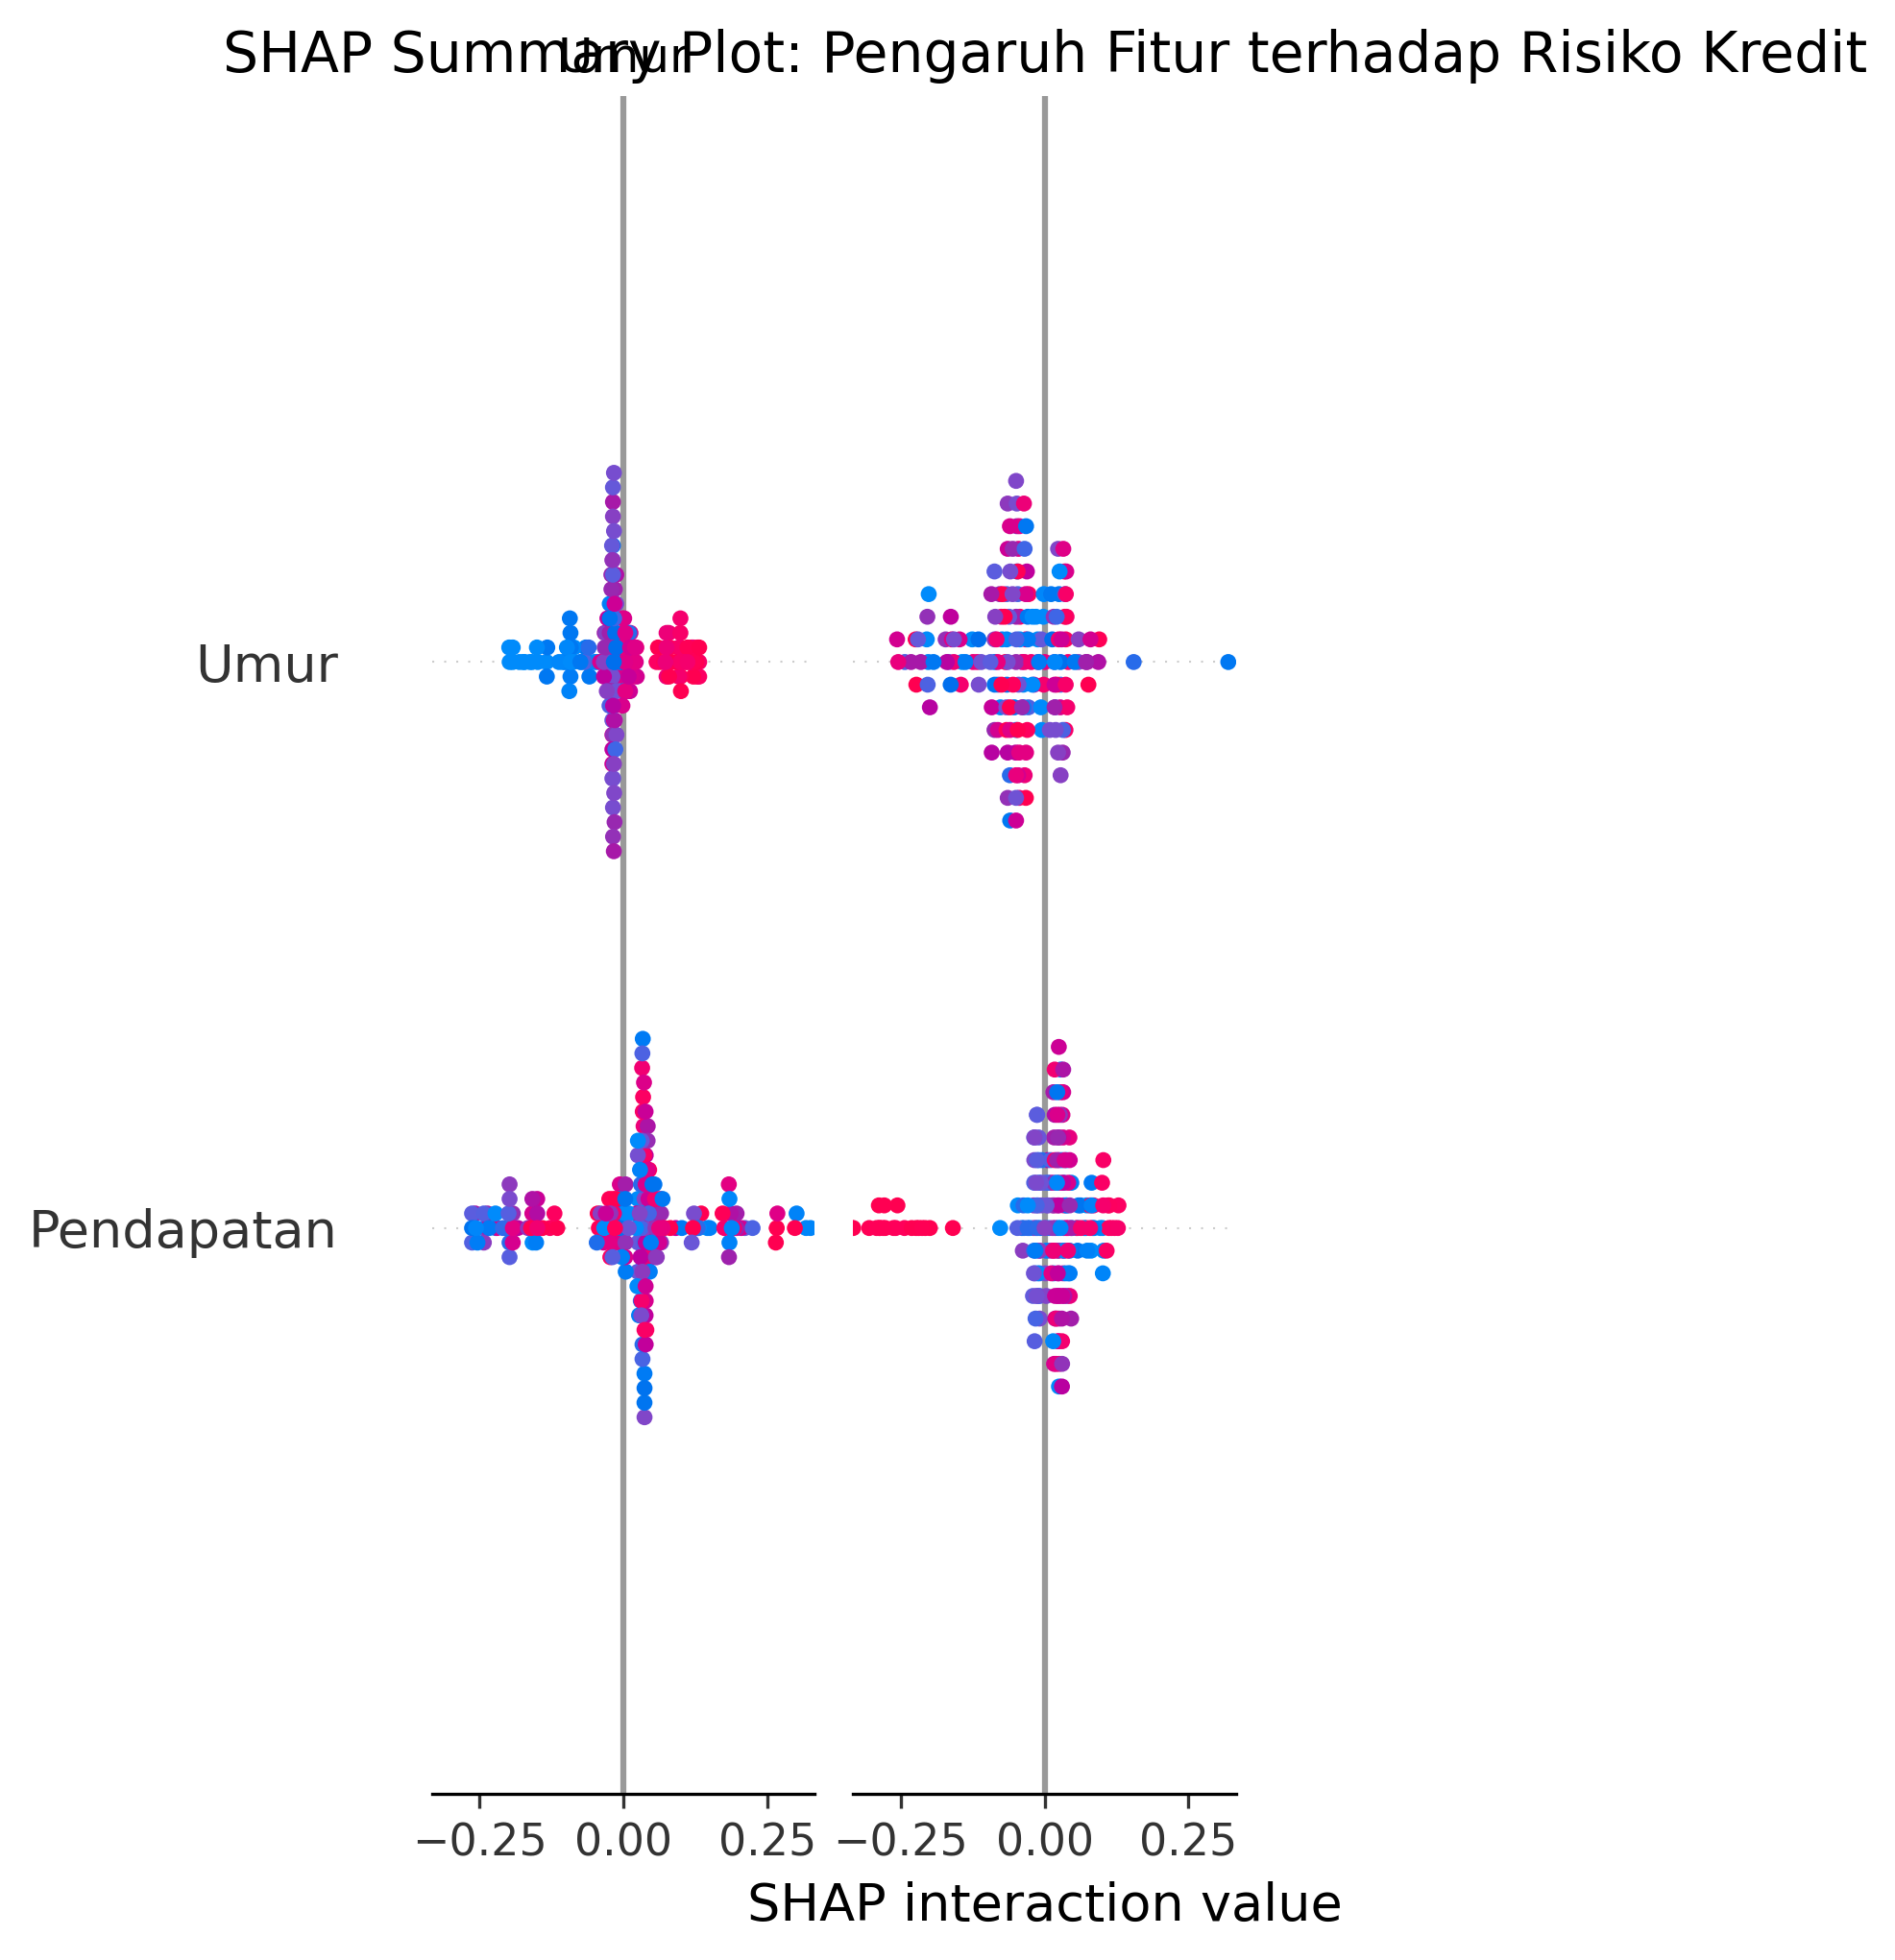
\includegraphics[width=0.76\textwidth]{bab4/shap_summary.png}
\caption{Ringkasan kontribusi fitur berdasarkan nilai SHAP}
\label{fig:bab4_shap_summary_detail}
\end{figure}


\section{Pengujian Perbandingan Skenario Model dan Studi Ablasi}
\label{sec:bab4_perbandingan_skenario}
Selain menguji model utama, penelitian ini juga melakukan studi ablasi (\textit{ablation study}) untuk mengevaluasi kontribusi transformasi \textit{Weight of Evidence} (WoE) dan penanganan ketidakseimbangan kelas menggunakan SMOTE. Studi ini dilakukan dengan membandingkan empat arsitektur model klasifikasi, yaitu Logistic Regression, Decision Tree, Random Forest, dan XGBoost.

Pengujian dilakukan pada empat konfigurasi data. Pertama, konfigurasi \textit{Full} menggunakan WoE dan SMOTE. Kedua, konfigurasi \textit{No SMOTE} menggunakan WoE tanpa penyeimbangan kelas. Ketiga, konfigurasi \textit{No WoE} menggunakan fitur mentah yang telah distandardisasi dan di-encode, kemudian diseimbangkan dengan SMOTE. Keempat, konfigurasi \textit{Raw} menggunakan fitur mentah tanpa WoE dan tanpa SMOTE. Perbandingan ini bertujuan melihat apakah peningkatan performa berasal dari model, transformasi fitur, penyeimbangan kelas, atau kombinasi ketiganya.

\begin{scriptsize}
\setlength{\tabcolsep}{3pt}
\renewcommand{\arraystretch}{1.1}
\begin{longtable}{p{0.18\textwidth} p{0.18\textwidth} c c c c c}
\caption{Perbandingan kinerja model dan studi ablasi}
\label{tab:bab4_ablation_study} \\
\toprule
\textbf{Konfigurasi Data} & \textbf{Arsitektur Model} & \textbf{ROC AUC} & \textbf{F1} & \textbf{Presisi} & \textbf{Recall} & \textbf{Waktu (s)} \\
\midrule
\endfirsthead
\multicolumn{7}{c}{{\tablename\ \thetable{} -- Lanjutan dari halaman sebelumnya}} \\
\toprule
\textbf{Konfigurasi Data} & \textbf{Arsitektur Model} & \textbf{ROC AUC} & \textbf{F1} & \textbf{Presisi} & \textbf{Recall} & \textbf{Waktu (s)} \\
\midrule
\endhead
\midrule
\multicolumn{7}{r}{{Bersambung ke halaman berikutnya...}} \\
\endfoot
\bottomrule
\endlastfoot
\textit{Full} (WoE + SMOTE) & Logistic Regression & 0,8098 & 0,7563 & 0,7996 & 0,7175 & 0,0193 \\
 & Decision Tree & 0,7961 & 0,7574 & 0,7865 & 0,7303 & 0,0146 \\
 & Random Forest & 0,8214 & 0,7739 & 0,8059 & 0,7443 & 0,4186 \\
 & \textbf{XGBoost} & \textbf{0,8284} & \textbf{0,7752} & \textbf{0,8055} & \textbf{0,7471} & \textbf{0,1652} \\
\midrule
\textit{No SMOTE} (WoE) & Logistic Regression & 0,8096 & 0,7899 & 0,7613 & 0,8208 & 0,0121 \\
 & Decision Tree & 0,8029 & 0,7775 & 0,7707 & 0,7845 & 0,0071 \\
 & Random Forest & 0,8249 & 0,8049 & 0,7433 & 0,8777 & 0,3622 \\
 & XGBoost & 0,8319 & 0,8069 & 0,7339 & 0,8961 & 0,1138 \\
\midrule
\textit{No WoE} (SMOTE) & Logistic Regression & 0,7813 & 0,7457 & 0,7855 & 0,7097 & 0,0115 \\
 & Decision Tree & 0,8021 & 0,7666 & 0,7985 & 0,7370 & 0,0273 \\
 & Random Forest & 0,8311 & 0,7737 & 0,8204 & 0,7320 & 0,6336 \\
 & XGBoost & 0,8379 & 0,7831 & 0,8181 & 0,7510 & 0,1277 \\
\midrule
\textit{Raw} & Logistic Regression & 0,7814 & 0,7705 & 0,7341 & 0,8107 & 0,0116 \\
 & Decision Tree & 0,8011 & 0,7712 & 0,7653 & 0,7772 & 0,0219 \\
 & Random Forest & 0,8224 & 0,7982 & 0,7428 & 0,8626 & 0,6064 \\
 & XGBoost & 0,8367 & 0,8071 & 0,7282 & 0,9051 & 0,2196 \\
\end{longtable}
\renewcommand{\arraystretch}{1}
\end{scriptsize}

Secara visual, perbandingan kurva ROC antararsitektur model pada konfigurasi utama ditunjukkan pada Gambar \ref{fig:bab4_roc_comparison}. Visualisasi ini digunakan untuk melihat kemampuan diskriminasi masing-masing model pada berbagai ambang keputusan.

\begin{figure}[H]
\centering
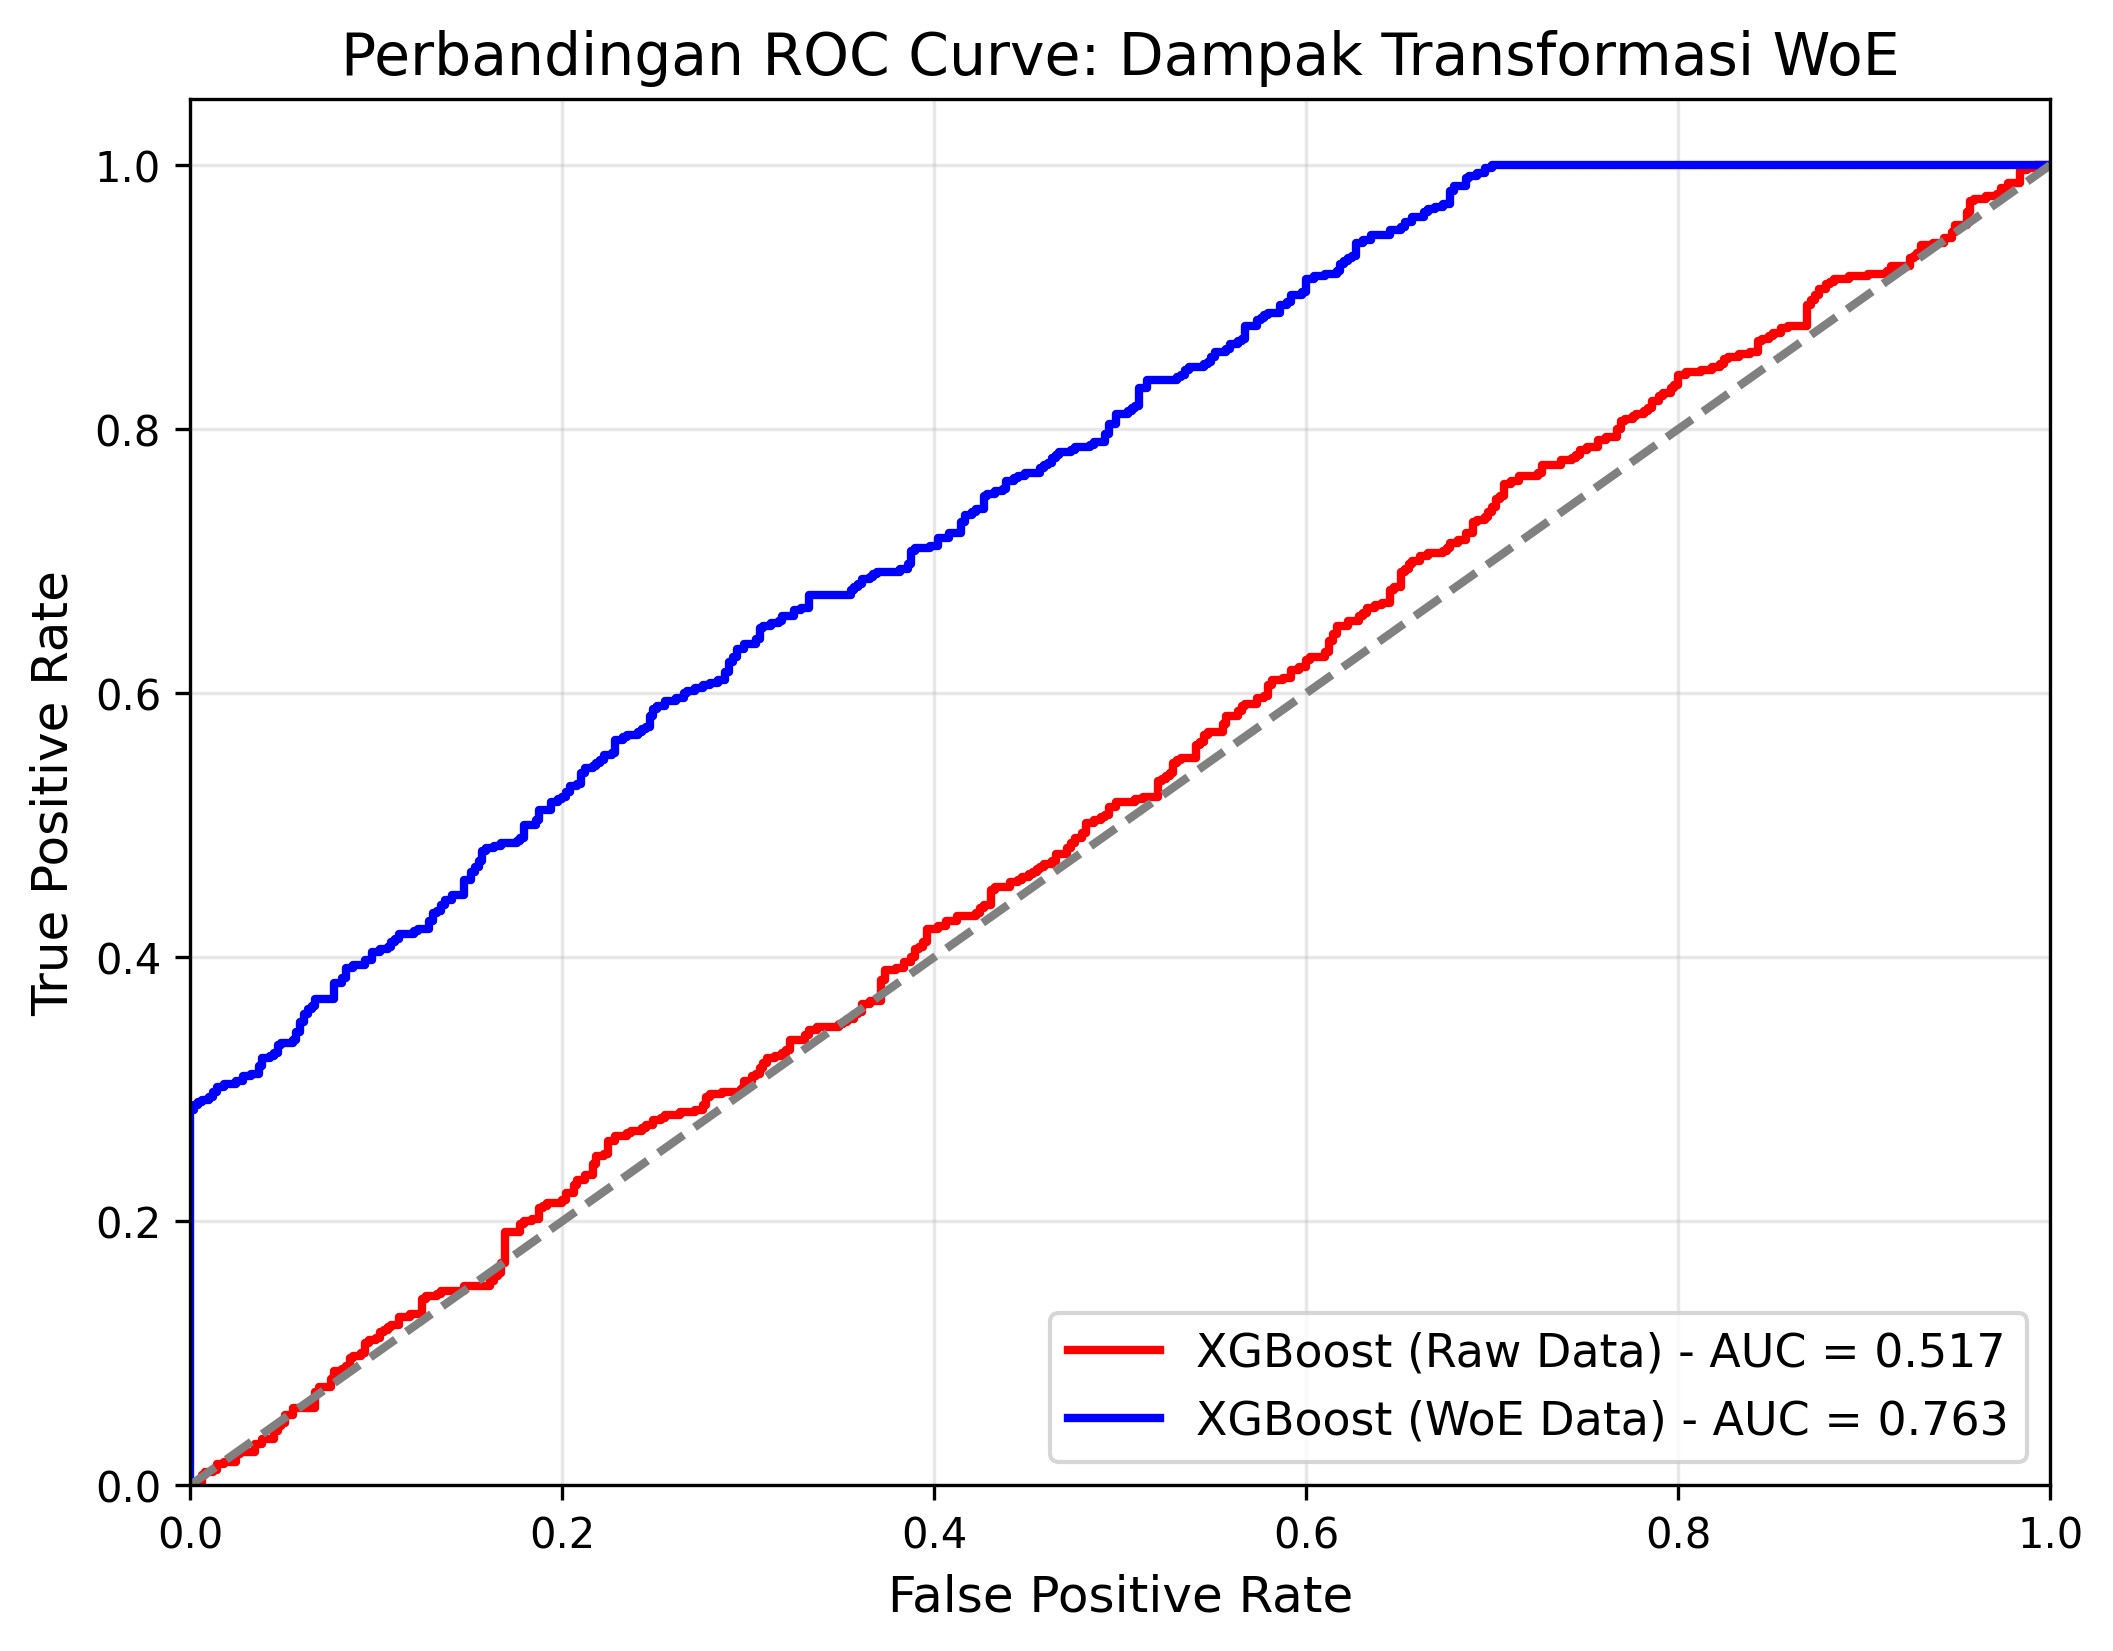
\includegraphics[width=0.8\textwidth]{bab4/roc_curve_comparison.png}
\caption{Perbandingan kurva ROC antara model dan skenario pengujian}
\label{fig:bab4_roc_comparison}
\end{figure}

\subsection{Analisis Dampak Transformasi Weight of Evidence}
Hasil studi ablasi menunjukkan bahwa transformasi WoE memberikan dampak yang berbeda antara model linear dan model berbasis pohon. Pada Logistic Regression, penggunaan WoE meningkatkan ROC AUC dari 0,7813 pada skenario \textit{No WoE} menjadi 0,8098 pada skenario \textit{Full}. Peningkatan ini terjadi karena WoE memetakan hubungan antara fitur dan peluang gagal bayar ke dalam bentuk yang lebih dekat dengan relasi log-odds, sehingga lebih sesuai dengan karakteristik model linear.

Pada model non-linear seperti XGBoost dan Random Forest, peniadaan WoE tidak selalu menurunkan ROC AUC. XGBoost pada skenario \textit{No WoE} memperoleh ROC AUC 0,8379, sedikit lebih tinggi dibandingkan skenario \textit{Full} sebesar 0,8284. Hal ini wajar karena model berbasis pohon mampu menangkap hubungan non-linear secara langsung dari fitur mentah. Namun, WoE tetap penting dalam konteks risiko kredit karena menghasilkan fitur yang lebih stabil, lebih mudah diaudit, dan lebih mudah dijelaskan kepada analis maupun pihak pengawas.

\subsection{Analisis Dampak SMOTE}
Penerapan SMOTE mengubah keseimbangan antara presisi dan recall model. Pada XGBoost dengan WoE tanpa SMOTE, recall mencapai 0,8961 tetapi presisi hanya 0,7339. Setelah SMOTE diterapkan pada konfigurasi \textit{Full}, presisi meningkat menjadi 0,8055, sedangkan recall menjadi 0,7471. Perubahan ini menunjukkan bahwa SMOTE menggeser batas keputusan model agar prediksi default menjadi lebih selektif dan tidak terlalu banyak menghasilkan peringatan risiko yang keliru.

Dalam konteks bisnis, peningkatan presisi penting karena dapat mengurangi kesalahan dalam menandai nasabah layak sebagai berisiko tinggi. Di sisi lain, recall 0,7471 masih menunjukkan bahwa model tetap mampu mendeteksi sebagian besar nasabah yang berpotensi gagal bayar. Oleh karena itu, konfigurasi \textit{Full} dipilih sebagai skenario yang lebih seimbang antara akurasi prediktif, stabilitas fitur, interpretabilitas, dan kebutuhan operasional.

\subsection{Analisis Interpretabilitas SHAP Lintas Model}
Untuk mengevaluasi konsistensi penjelasan model, dilakukan analisis SHAP pada konfigurasi \textit{Full}. Gambar \ref{fig:bab4_shap_lr} sampai Gambar \ref{fig:bab4_shap_xgb} menunjukkan ringkasan kontribusi fitur untuk Logistic Regression, Decision Tree, Random Forest, dan XGBoost.

\begin{figure}[H]
\centering
\begin{minipage}{0.48\textwidth}
\centering
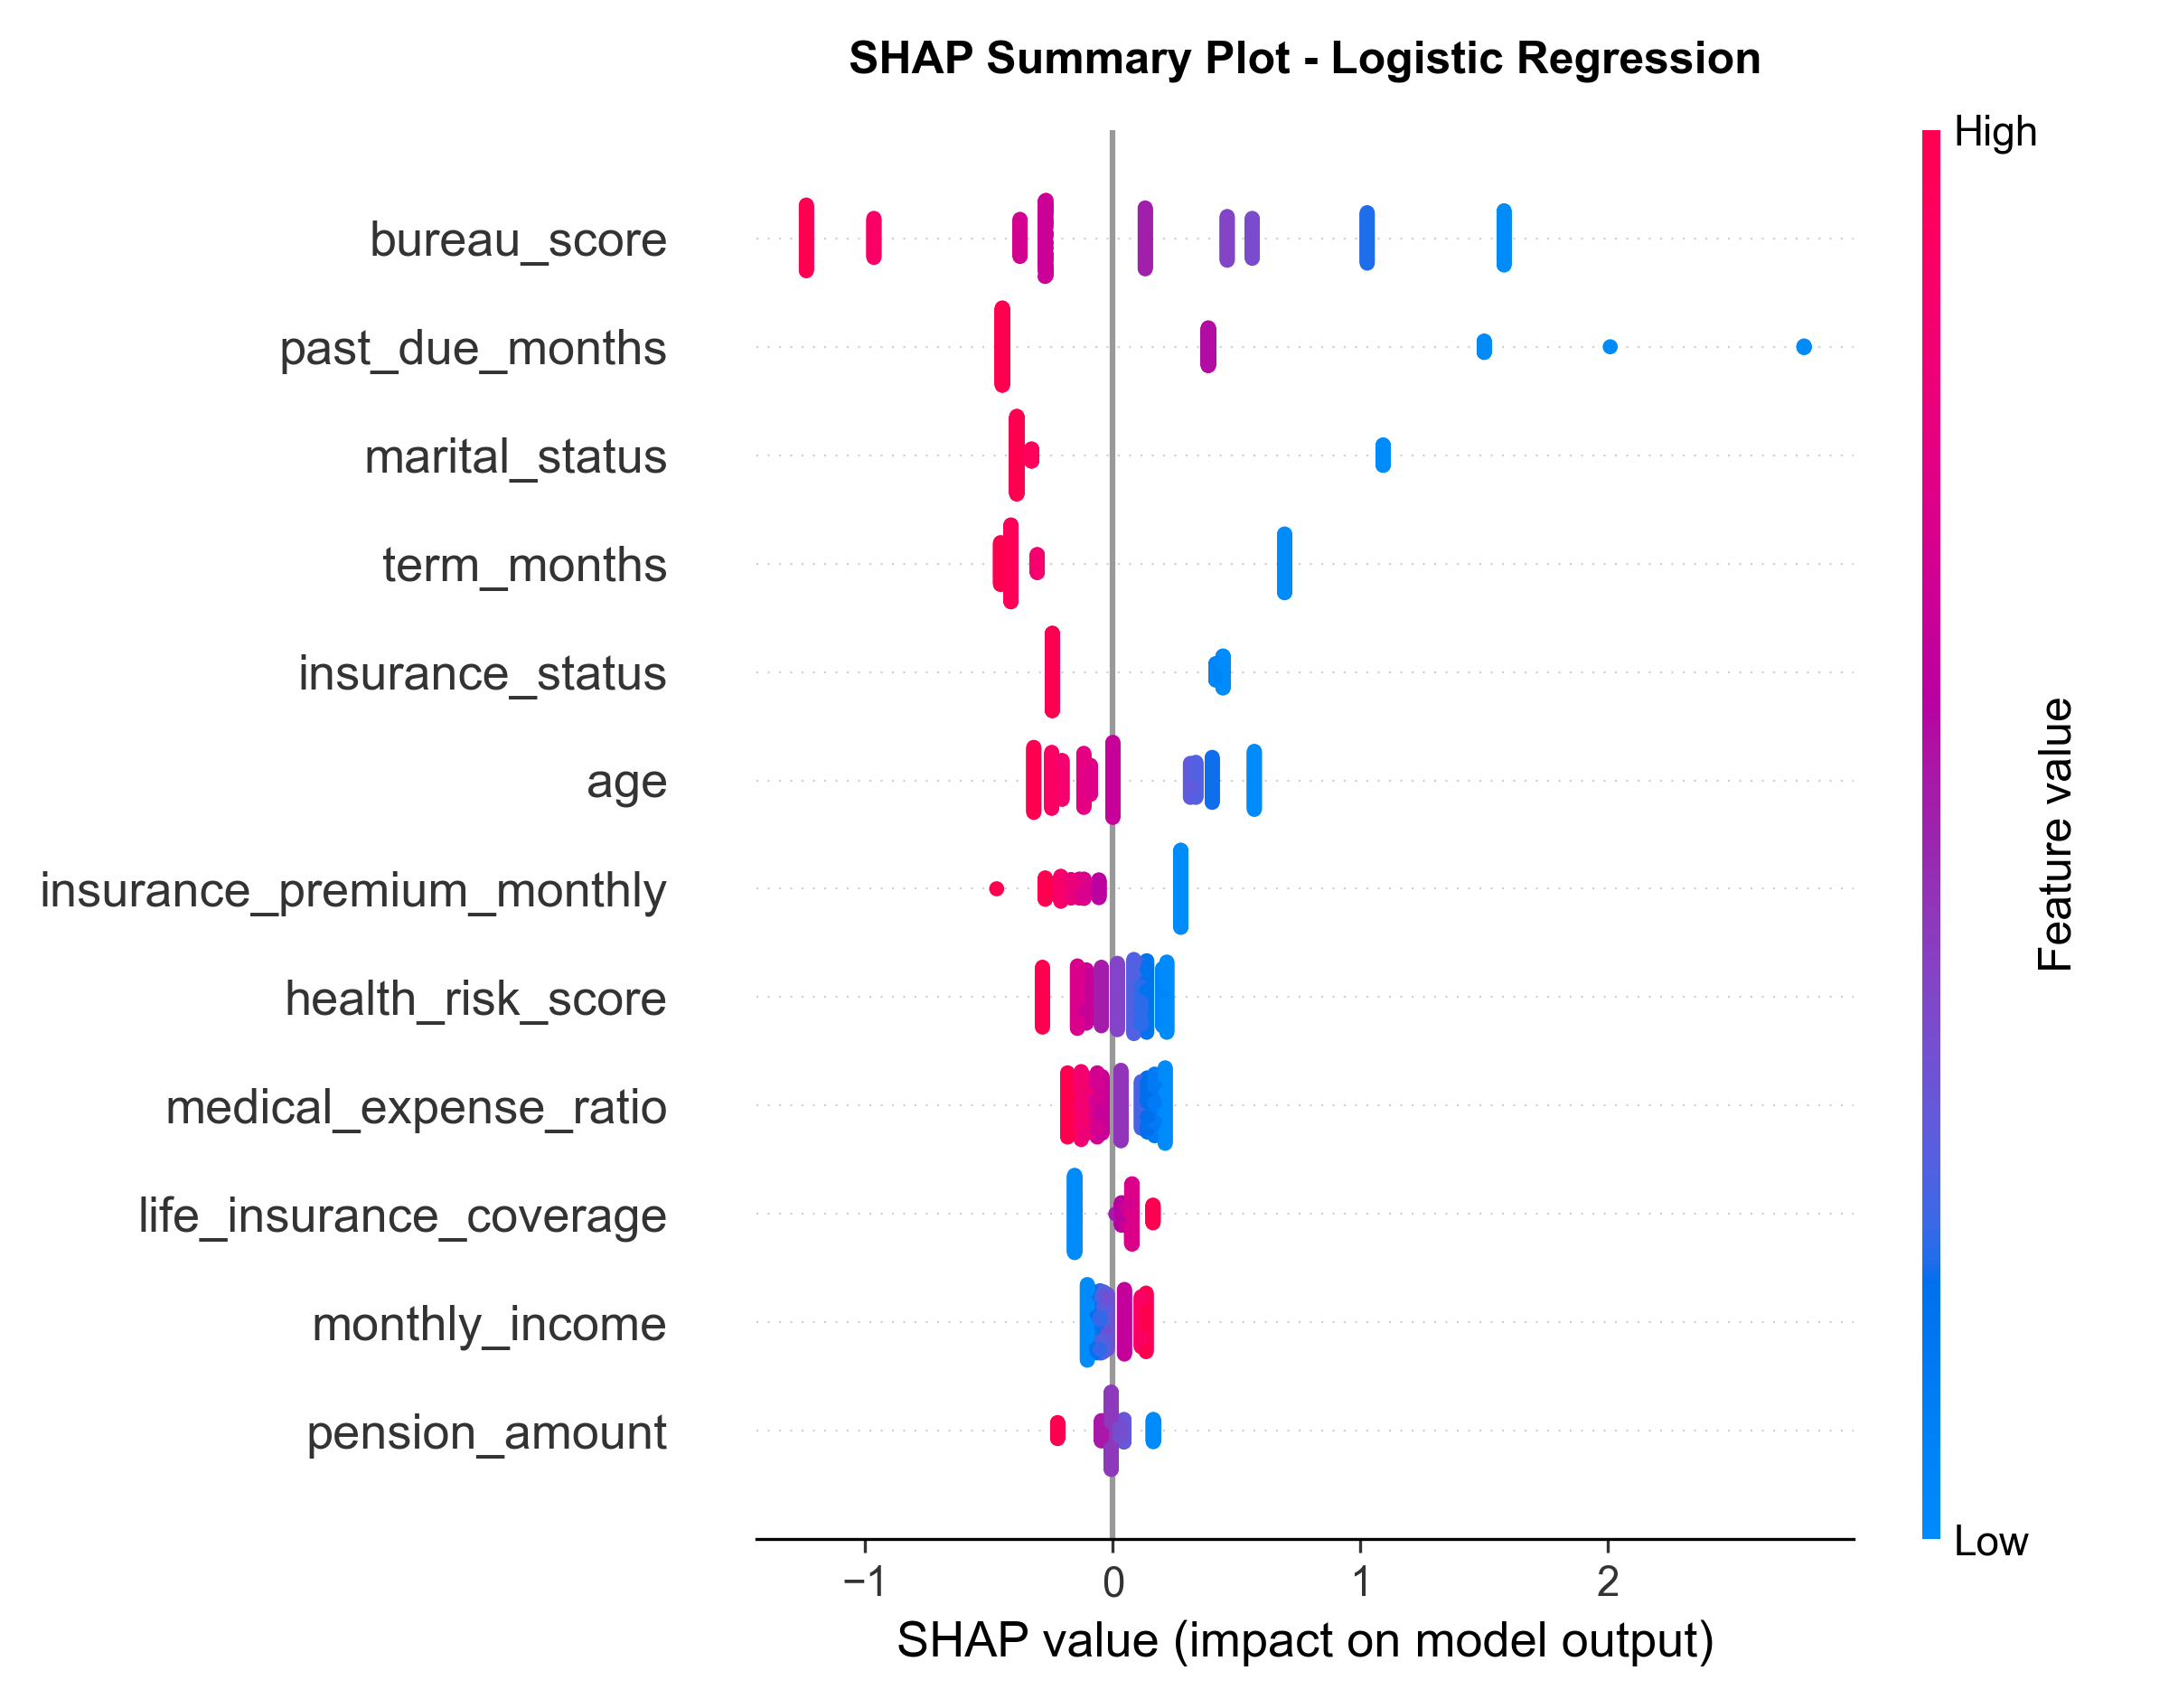
\includegraphics[width=\textwidth]{bab4/SHAP_Summary_LogisticRegression.png}
\caption{SHAP summary Logistic Regression}
\label{fig:bab4_shap_lr}
\end{minipage}
\hfill
\begin{minipage}{0.48\textwidth}
\centering
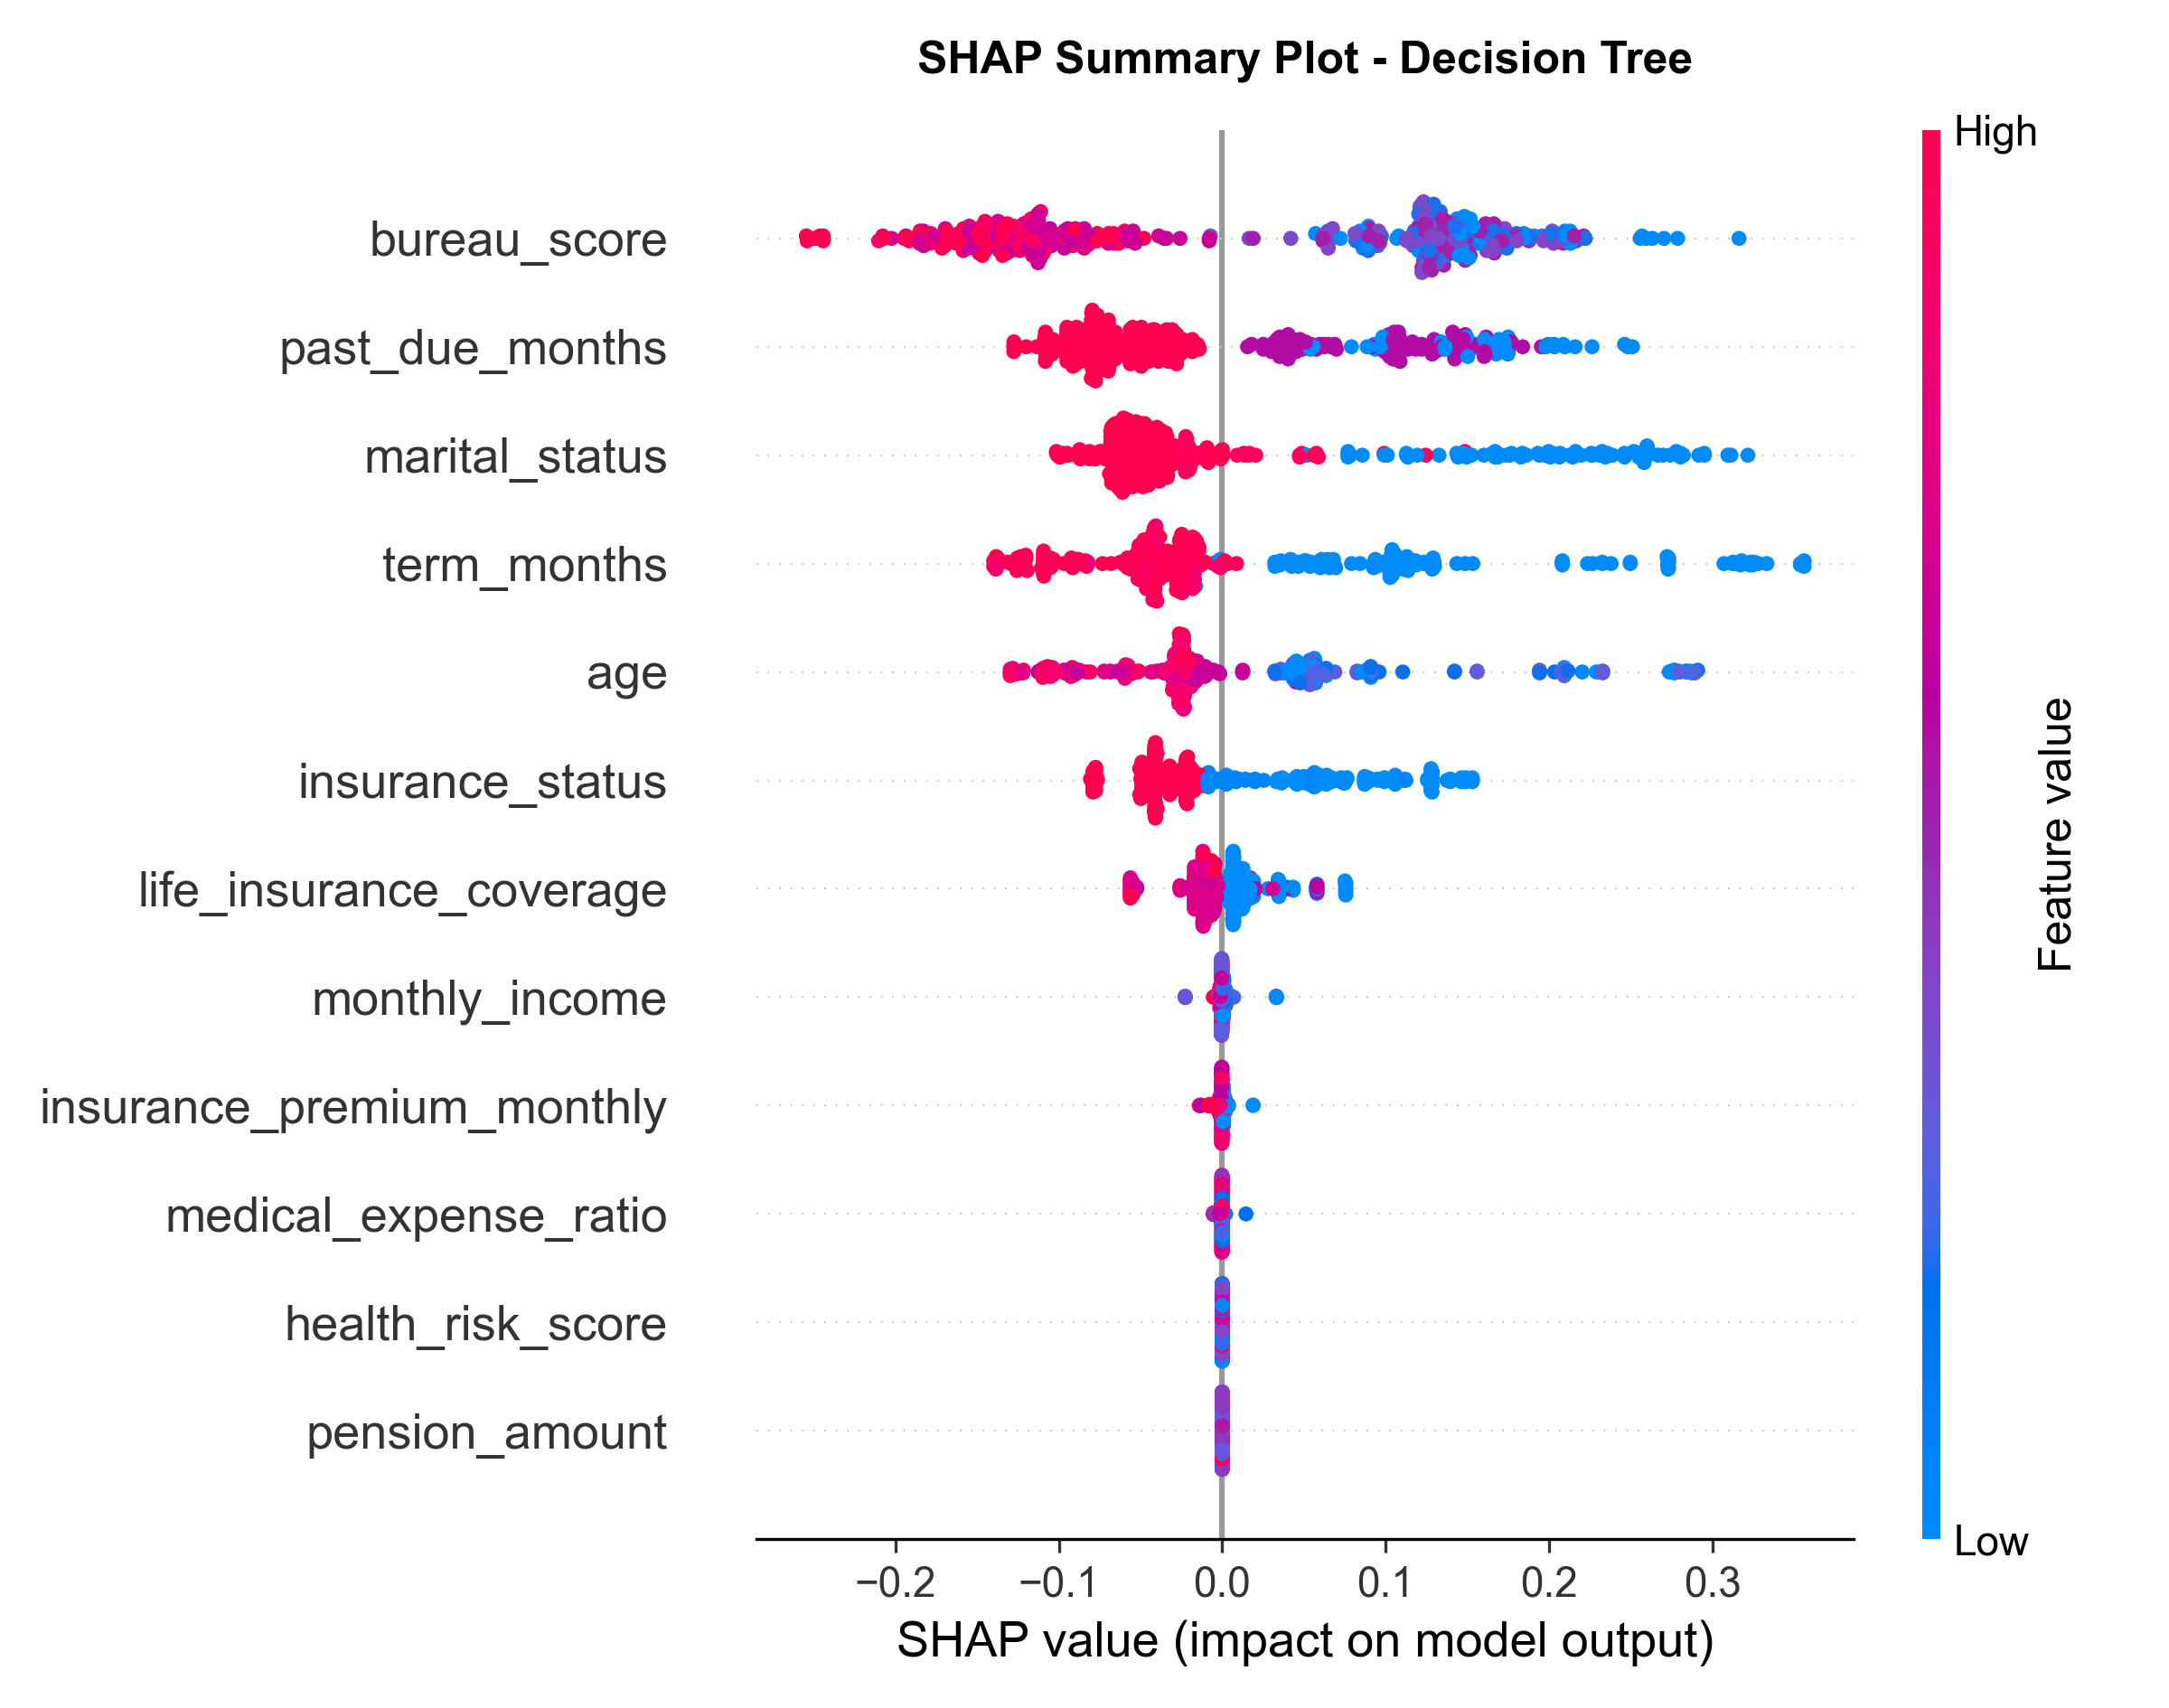
\includegraphics[width=\textwidth]{bab4/SHAP_Summary_DecisionTree.png}
\caption{SHAP summary Decision Tree}
\label{fig:bab4_shap_dt}
\end{minipage}
\end{figure}

\begin{figure}[H]
\centering
\begin{minipage}{0.48\textwidth}
\centering
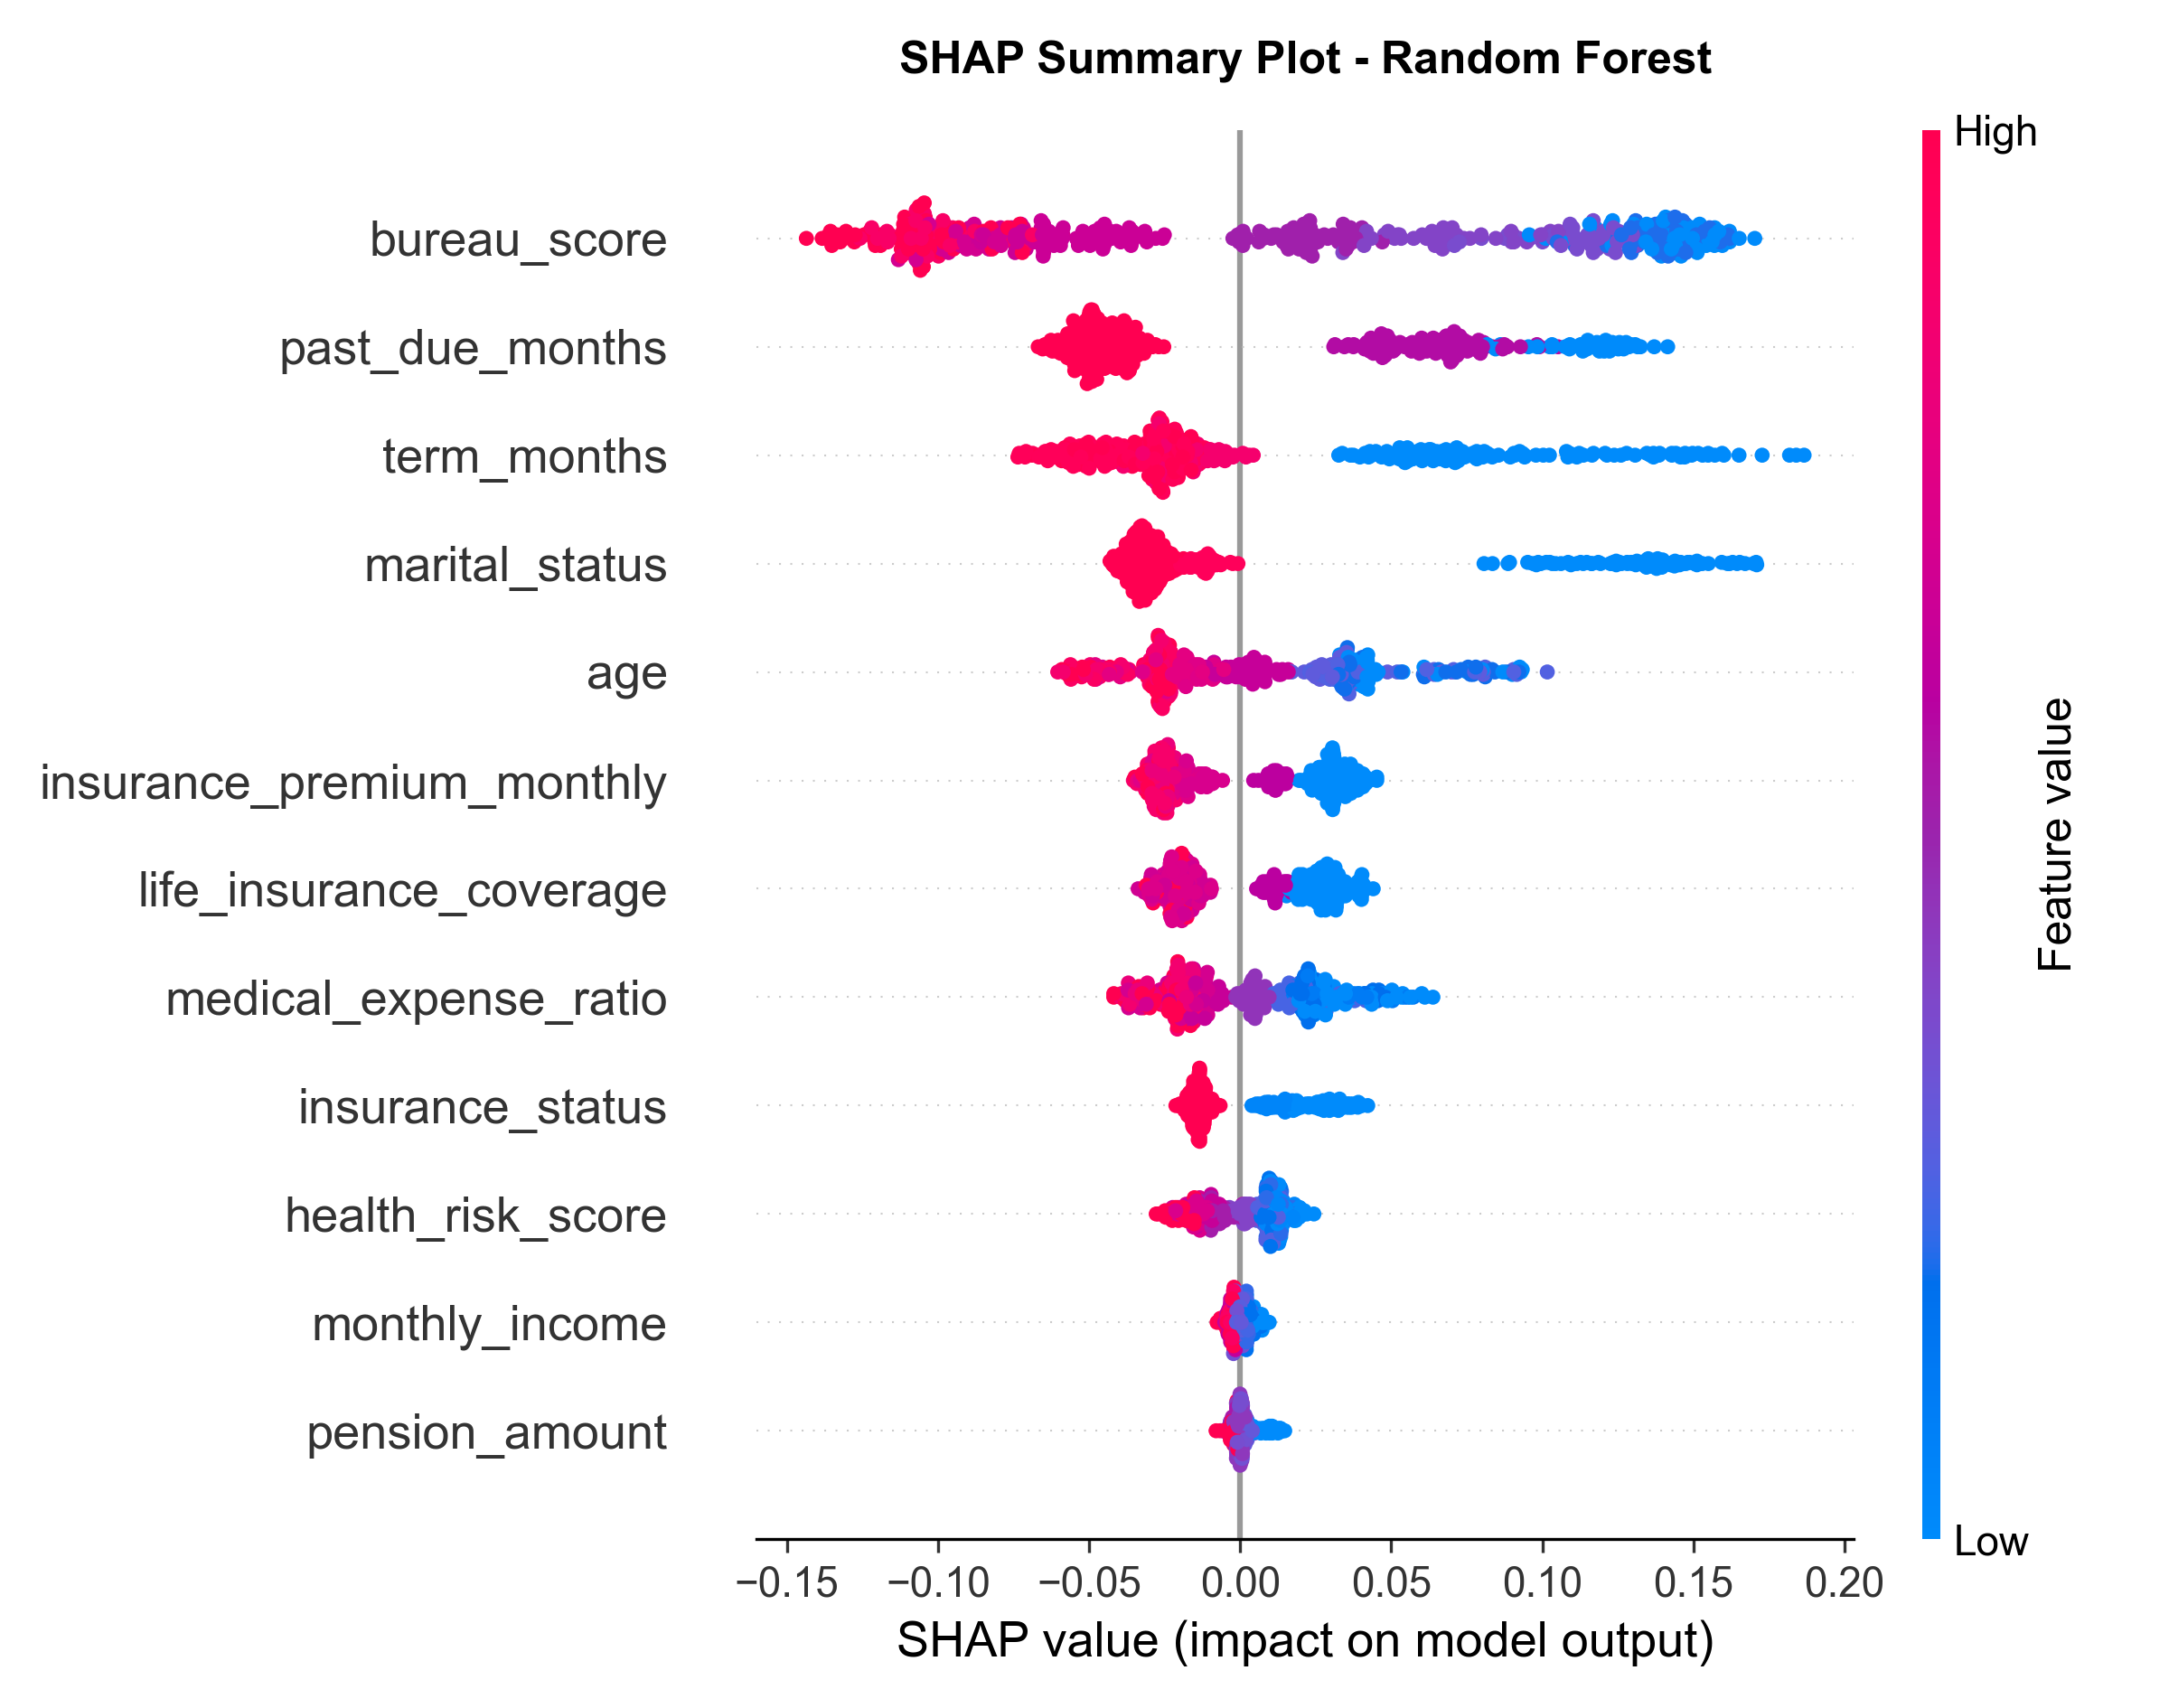
\includegraphics[width=\textwidth]{bab4/SHAP_Summary_RandomForest.png}
\caption{SHAP summary Random Forest}
\label{fig:bab4_shap_rf}
\end{minipage}
\hfill
\begin{minipage}{0.48\textwidth}
\centering
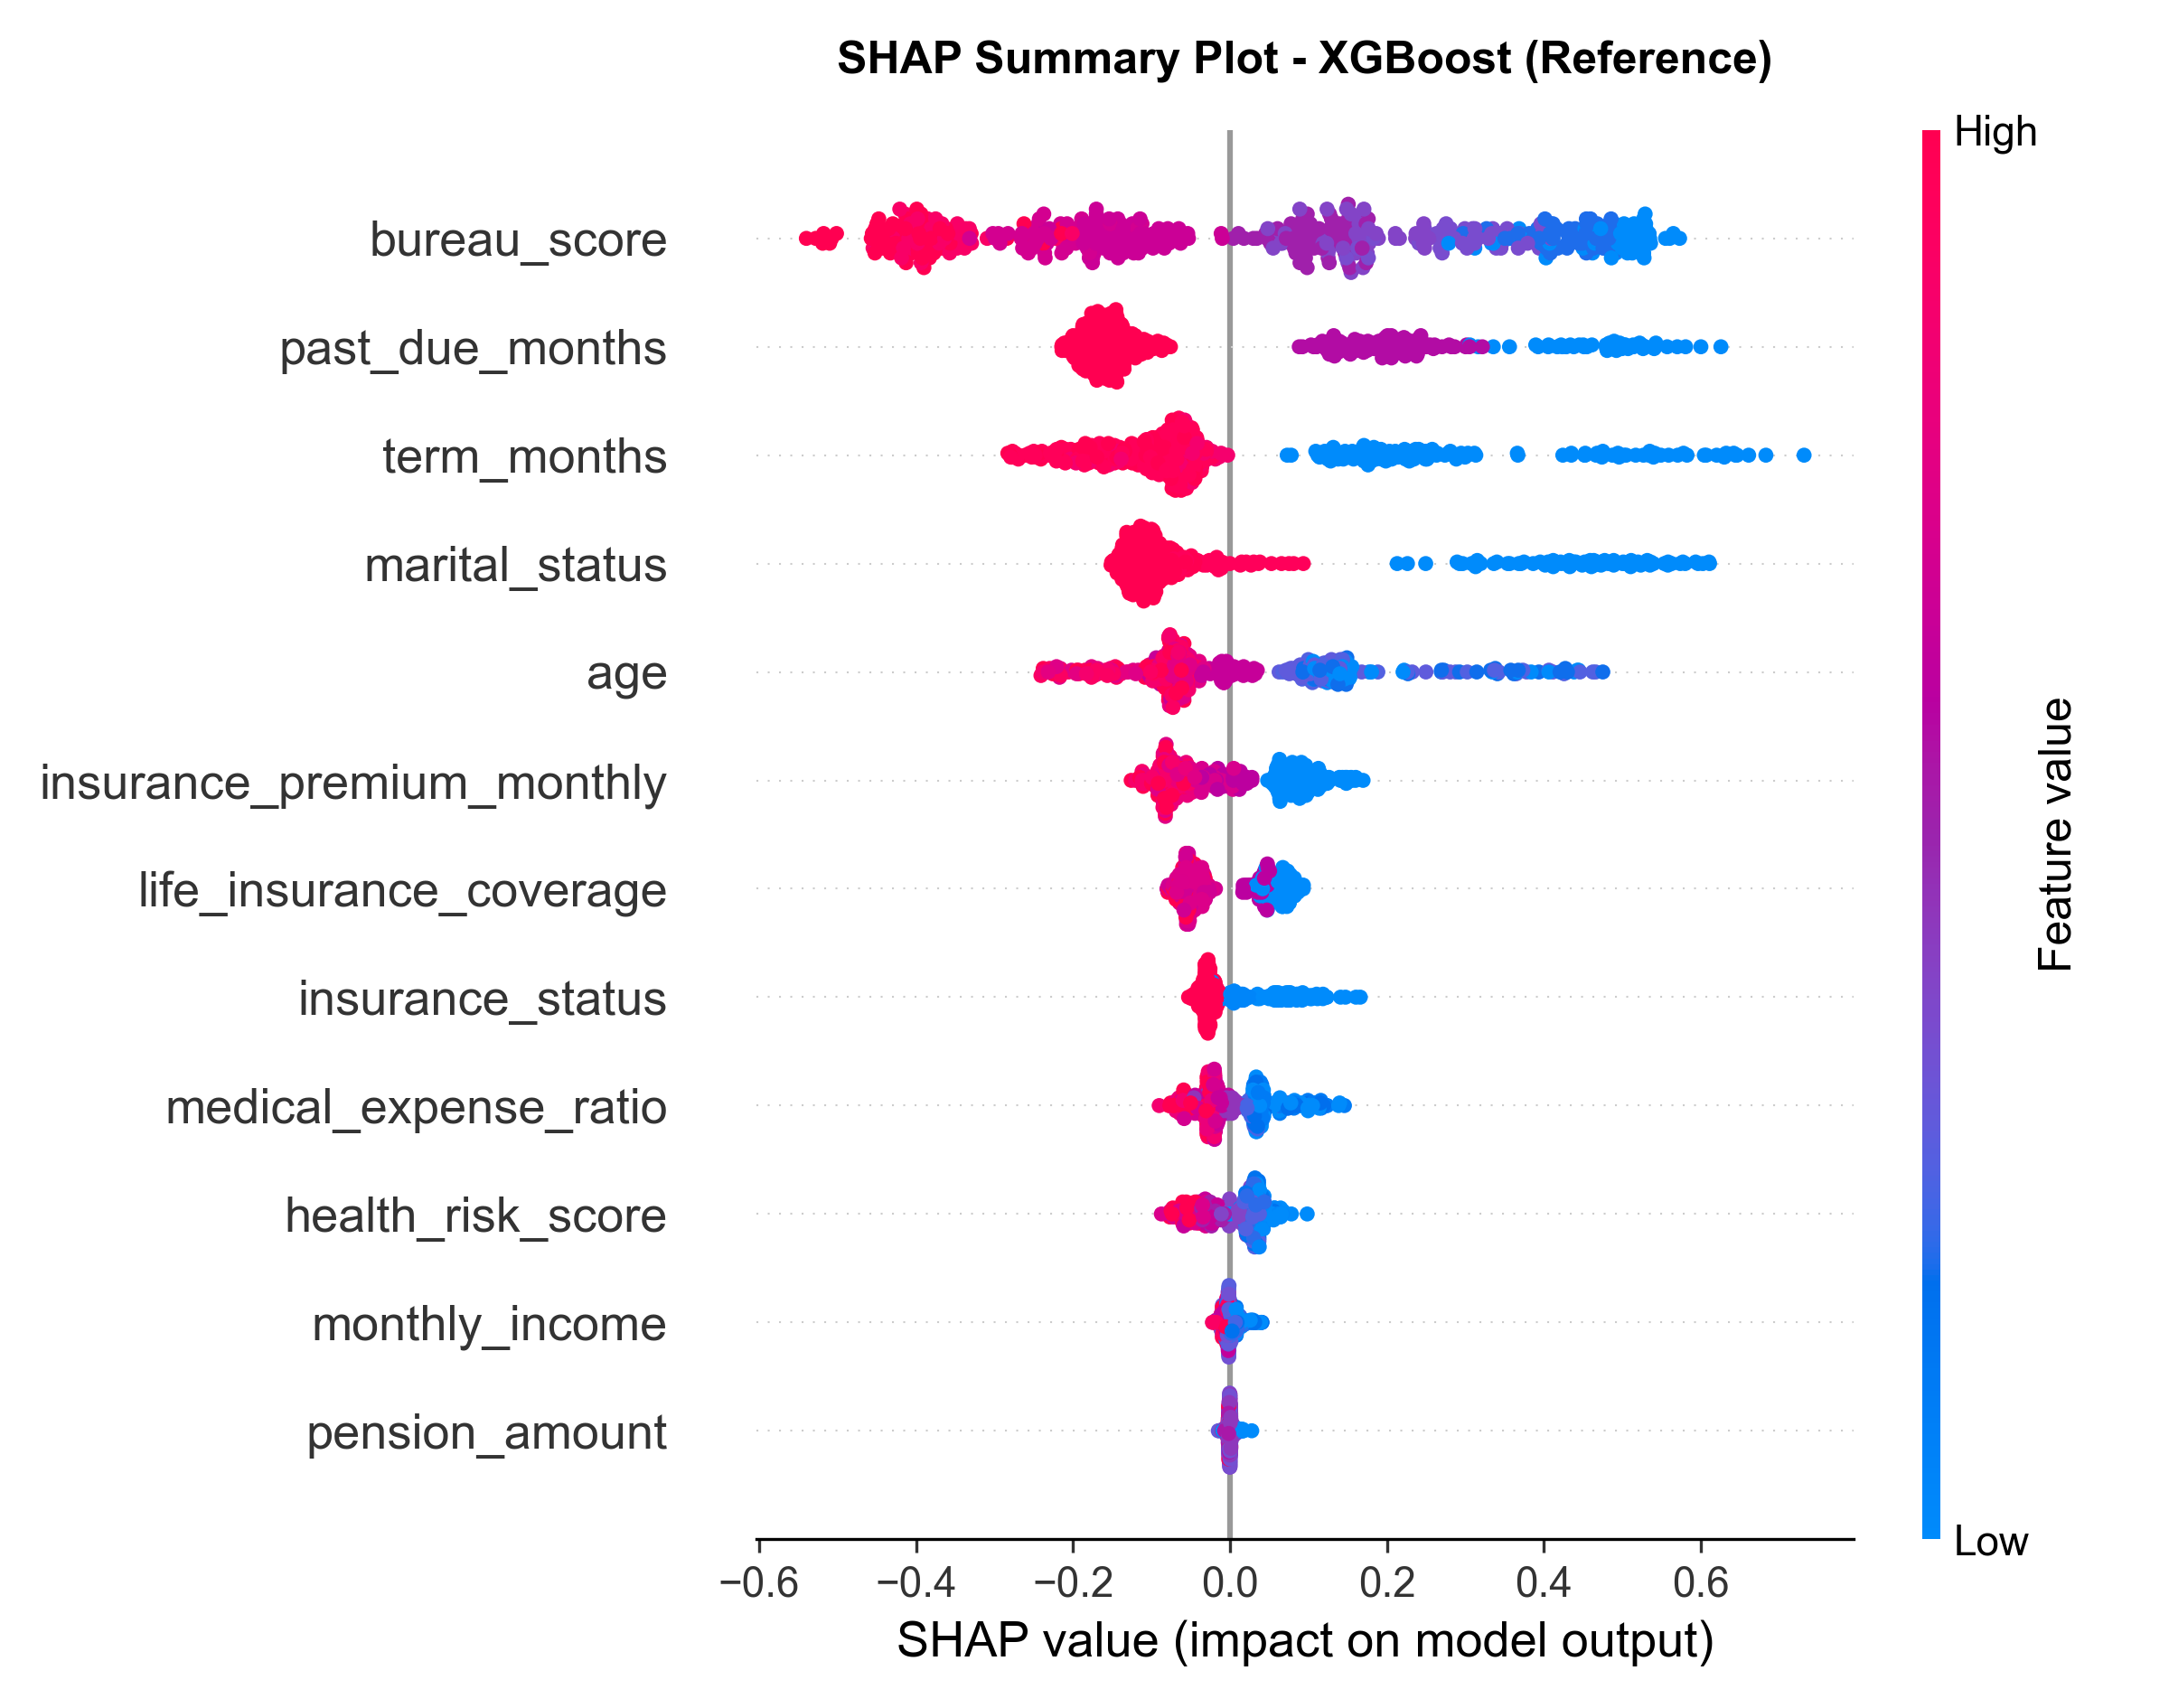
\includegraphics[width=\textwidth]{bab4/SHAP_Summary_XGBoost.png}
\caption{SHAP summary XGBoost}
\label{fig:bab4_shap_xgb}
\end{minipage}
\end{figure}

Hasil interpretasi menunjukkan bahwa \textit{bureau\_score} menjadi fitur paling dominan pada seluruh model. Fitur \textit{past\_due\_months} juga konsisten berada pada peringkat atas, yang menunjukkan bahwa histori keterlambatan pembayaran merupakan sinyal penting dalam memprediksi gagal bayar. Selain itu, \textit{marital\_status} dan \textit{term\_months} memberikan pengaruh menengah, sedangkan fitur seperti \textit{monthly\_income} dan \textit{pension\_amount} berperan sebagai penyesuaian tambahan terhadap profil risiko nasabah.

Konsistensi kontribusi fitur antar model menunjukkan bahwa pipeline berbasis WoE tidak hanya menghasilkan performa prediktif yang kompetitif, tetapi juga menjaga koherensi interpretasi. Dengan demikian, penggunaan XGBoost sebagai model referensi tetap dapat dijustifikasi karena hasil prediksinya selaras dengan faktor risiko yang logis dalam konteks penilaian kredit.

\section{Pengujian API Serving dan Aturan Bisnis}
\label{sec:bab4_api_serving}
Model terbaik yang telah dipilih kemudian diuji melalui layanan FastAPI pada endpoint \textit{/predict}. Pengujian ini bertujuan memastikan bahwa model dapat menerima input dalam format JSON, mengembalikan skor risiko, menghasilkan grade, serta menyertakan penjelasan berbasis SHAP untuk mendukung transparansi keputusan.

Pada kasus uji pertama, nasabah berusia 48 tahun dengan \textit{bureau\_score} 750, pendapatan bulanan Rp8.500.000, tenor 24 bulan, DTI 0,25, dan tidak memiliki tunggakan diprediksi memiliki probabilitas gagal bayar sebesar 0,0845. Sistem mengembalikan Grade A, yang menunjukkan bahwa nasabah tergolong sangat layak. Nilai SHAP menunjukkan bahwa \textit{bureau\_score} dan \textit{insurance\_status} berkontribusi dalam menurunkan risiko.

\begin{table}[H]
\centering
\caption{Hasil pengujian API untuk nasabah normal}
\label{tab:bab4_api_normal}
\begin{tabular}{|l|l|}
\hline
\textbf{Aspek} & \textbf{Hasil} \\
\hline
Usia & 48 tahun \\
\hline
Bureau score & 750 \\
\hline
DTI & 0,25 \\
\hline
Probabilitas default & 0,0845 \\
\hline
Grade & A \\
\hline
Interpretasi & Nasabah sangat layak karena risiko gagal bayar rendah. \\
\hline
\end{tabular}
\end{table}

Pada kasus uji kedua, sistem diuji dengan aturan bisnis batas usia pelunasan maksimal 80 tahun. Nasabah berusia 75 tahun mengajukan tenor 120 bulan, sehingga usia saat pelunasan menjadi 85 tahun. Walaupun model memprediksi probabilitas gagal bayar rendah, yaitu 0,0214, sistem tetap menetapkan Grade Undefined karena permohonan melanggar aturan bisnis keras.

\begin{table}[H]
\centering
\caption{Hasil pengujian API untuk pelanggaran aturan usia pelunasan}
\label{tab:bab4_api_rule}
\begin{tabular}{|l|l|}
\hline
\textbf{Aspek} & \textbf{Hasil} \\
\hline
Usia awal & 75 tahun \\
\hline
Tenor & 120 bulan \\
\hline
Usia saat pelunasan & 85 tahun \\
\hline
Probabilitas model & 0,0214 \\
\hline
Output akhir & Grade Undefined \\
\hline
Alasan anomali & Usia saat pelunasan melebihi batas 80 tahun. \\
\hline
\end{tabular}
\end{table}

Hasil ini membuktikan bahwa sistem tidak hanya mengandalkan model machine learning, tetapi juga menerapkan aturan bisnis yang bersifat wajib. Dalam konteks perbankan, mekanisme seperti ini penting karena keputusan kredit tidak boleh sepenuhnya diserahkan pada model statistik ketika terdapat batasan regulasi atau kebijakan internal yang harus dipatuhi.

Antarmuka web yang digunakan untuk menguji layanan prediksi ditunjukkan pada Gambar \ref{fig:bab4_web_prediction}. Tampilan tersebut memperlihatkan bahwa pengguna dapat memasukkan atribut calon nasabah, seperti \textit{bureau score}, usia, status pernikahan, tipe pekerjaan, nilai pinjaman, dan tenor. Setelah tombol analisis dijalankan, sistem menampilkan probabilitas gagal bayar, grade risiko, serta daftar kontribusi fitur berbasis SHAP. Hasil ini menunjukkan bahwa layanan FastAPI tidak hanya dapat dipanggil secara teknis, tetapi juga dapat diintegrasikan ke dalam antarmuka pengguna yang lebih mudah dipahami oleh analis kredit.

\begin{figure}[H]
\centering
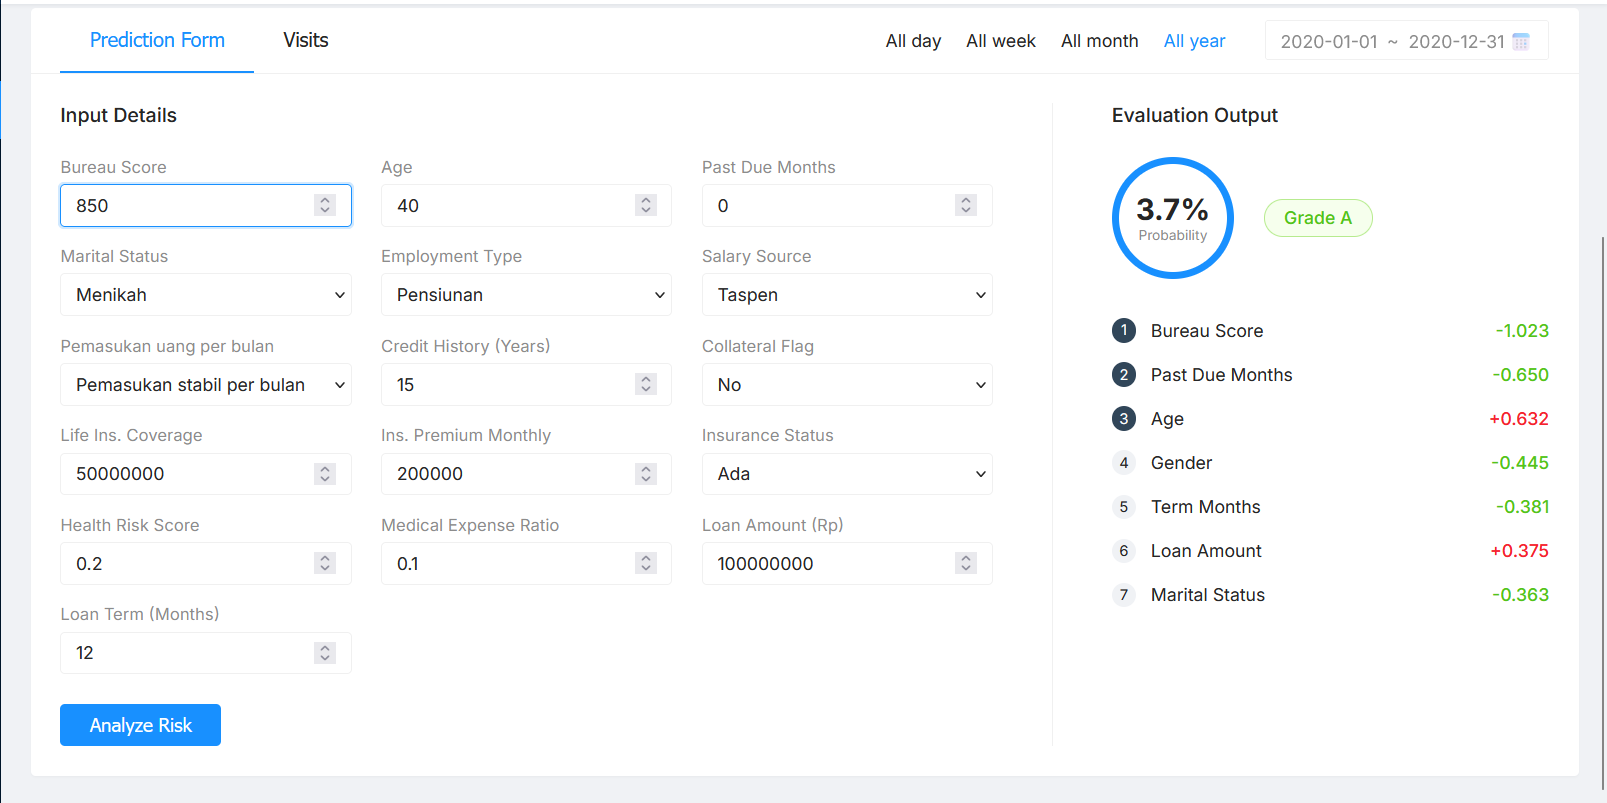
\includegraphics[width=0.92\textwidth]{bab4/Screenshot 2026-05-25 171508.png}
\caption{Antarmuka web untuk pengujian prediksi risiko kredit}
\label{fig:bab4_web_prediction}
\end{figure}


\subsection{Pengujian Arsitektur Database Nasabah}
Selain layanan prediksi, sistem juga dilengkapi dengan database operasional berbasis SQLite bernama \textit{nasabah.db} yang dikelola melalui modul \textit{database.py}. Database ini digunakan sebagai penyimpanan persisten untuk data nasabah, hasil prediksi risiko kredit, status persetujuan, serta log pengiriman email konfirmasi. Pada saat startup pertama, tabel utama diinisialisasi dari dataset sintetis sehingga data yang digunakan pada antarmuka web dan API tetap konsisten dengan data pengujian model.

Secara umum, database terdiri dari dua tabel utama, yaitu tabel \textit{nasabah} dan tabel \textit{sent\_emails}. Tabel \textit{nasabah} menyimpan atribut identitas, pekerjaan, kondisi finansial, kesehatan, asuransi, detail pinjaman, indikator transaksi, output model, status keputusan, dan variabel makroekonomi. Sementara itu, tabel \textit{sent\_emails} berfungsi sebagai log audit untuk mencatat email konfirmasi yang dikirim kepada pihak penanggung jawab persetujuan kredit.

\begin{table}[H]
\centering
\caption{Ringkasan tabel utama pada database \textit{nasabah.db}}
\label{tab:bab4_database_tables}
\begin{tabular}{|p{0.22\textwidth}|p{0.26\textwidth}|p{0.42\textwidth}|}
\hline
\textbf{Tabel} & \textbf{Kunci Utama} & \textbf{Fungsi} \\
\hline
\textit{nasabah} & \textit{customer\_id} & Menyimpan data nasabah, atribut kredit, hasil prediksi PD/LGD/EAD, risk grade, dan status persetujuan. \\
\hline
\textit{sent\_emails} & \textit{id} & Mencatat riwayat pengiriman email konfirmasi, penerima email, subjek, isi HTML, waktu kirim, dan relasi ke \textit{customer\_id}. \\
\hline
\end{tabular}
\end{table}

Struktur tabel \textit{nasabah} dikelompokkan menjadi beberapa kategori atribut. Kelompok identitas mencakup \textit{customer\_id}, \textit{loan\_id}, \textit{name\_masked}, usia, gender, dan status pernikahan. Kelompok pekerjaan dan pendapatan mencakup tipe pekerjaan, status pensiun, pendapatan bulanan, sumber gaji, stabilitas pendapatan, dan volatilitas gaji. Kelompok kesehatan finansial mencakup saldo rata-rata, jumlah cicilan aktif, DTI, \textit{bureau\_score}, tunggakan, dan panjang riwayat kredit. Selain itu, database juga menyimpan atribut kesehatan dan asuransi, detail pinjaman, perilaku transaksi, output model berupa PD, LGD, EAD, \textit{expected loss}, \textit{risk grade}, serta status keputusan \textit{Pending}, \textit{Accepted}, atau \textit{Rejected}.

\begin{table}[H]
\centering
\caption{Mapping endpoint REST API ke operasi database}
\label{tab:bab4_database_crud}
\begin{tabular}{|p{0.14\textwidth}|p{0.38\textwidth}|p{0.36\textwidth}|}
\hline
\textbf{Metode} & \textbf{Endpoint} & \textbf{Fungsi Operasional} \\
\hline
GET & \textit{/api/nasabah} & Mengambil daftar nasabah dengan dukungan pencarian, filter, dan paginasi. \\
\hline
GET & \textit{/api/nasabah/\{id\}} & Mengambil detail satu nasabah berdasarkan identitas nasabah. \\
\hline
POST & \textit{/api/nasabah} & Menambahkan data nasabah baru, termasuk data hasil ingestion dokumen. \\
\hline
PUT & \textit{/api/nasabah/\{id\}} & Memperbarui data nasabah dan atribut pendukung analisis kredit. \\
\hline
DELETE & \textit{/api/nasabah/\{id\}} & Menghapus data nasabah dari database. \\
\hline
GET & \textit{/api/nasabah/\{id\}/approve} & Memperbarui \textit{approval\_status} menjadi \textit{Accepted}. \\
\hline
GET & \textit{/api/nasabah/\{id\}/reject} & Memperbarui \textit{approval\_status} menjadi \textit{Rejected}. \\
\hline
POST & \textit{/api/nasabah/\{id\}/send-confirmation} & Mengirim email konfirmasi dan mencatat log ke tabel \textit{sent\_emails}. \\
\hline
GET & \textit{/api/sent-emails} & Mengambil riwayat email konfirmasi yang telah dikirim. \\
\hline
\end{tabular}
\end{table}

Pengujian database menunjukkan bahwa sistem tidak hanya berfungsi sebagai endpoint prediksi, tetapi juga sebagai aplikasi operasional sederhana untuk manajemen data kredit. Mekanisme CRUD memungkinkan data dari antarmuka web maupun ingestion PDF disimpan ke tabel yang sama, sedangkan status persetujuan memberikan ruang bagi proses \textit{human-in-the-loop}. Setiap email konfirmasi yang dikirim dicatat dalam tabel \textit{sent\_emails}, sehingga proses eskalasi keputusan memiliki jejak audit yang dapat ditelusuri kembali.

\subsection{Pengujian Otomasi Ingestion PDF dan Konfirmasi Email}
Selain pengujian prediksi melalui antarmuka web, sistem juga diuji pada skenario otomasi berbasis email untuk memperluas cakupan operasional pipeline. Skenario pertama adalah ingestion formulir kredit dalam format PDF melalui workflow n8n. Pada skenario ini, email masuk yang memiliki lampiran PDF formulir kredit diproses oleh workflow n8n, kemudian lampiran tersebut dibaca dan diekstraksi menjadi data terstruktur sebelum dikirimkan ke layanan backend untuk disimpan sebagai data nasabah baru. Mekanisme ini menunjukkan bahwa pipeline tidak hanya menerima input manual dari antarmuka web, tetapi juga mampu mengakomodasi alur pengajuan berbasis dokumen yang umum digunakan dalam proses administratif kredit.

\begin{figure}[H]
\centering
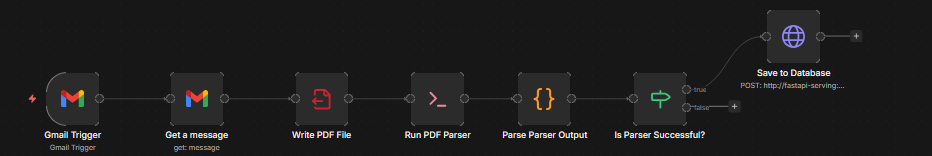
\includegraphics[width=0.92\textwidth]{bab4/Email_PDF_pipeline.png}
\caption{Workflow n8n untuk ingestion formulir kredit PDF melalui email}
\label{fig:bab4_email_pdf_pipeline}
\end{figure}

Skenario kedua adalah pengiriman email konfirmasi kepada pihak yang bertanggung jawab dalam proses persetujuan kredit. Setelah data nasabah dan hasil analisis risiko tersedia, sistem dapat mengirimkan email konfirmasi yang berisi ringkasan informasi pengajuan, hasil penilaian risiko, serta opsi tindak lanjut. Alur ini mendukung proses \textit{human-in-the-loop} karena keputusan akhir tidak sepenuhnya diserahkan kepada model, melainkan tetap dapat ditinjau oleh analis atau pihak berwenang sebelum status persetujuan diperbarui.

\begin{table}[H]
\centering
\caption{Kasus uji konfirmasi email dan keputusan manual}
\label{tab:bab4_email_hitl_test}
\begin{tabular}{|p{0.28\textwidth}|p{0.62\textwidth}|}
\hline
\textbf{Aspek Pengujian} & \textbf{Hasil yang Diharapkan} \\
\hline
Pemicu email & Endpoint \textit{/api/nasabah/\{id\}/send-confirmation} mengirim ringkasan risiko kepada reviewer. \\
\hline
Isi email & Email memuat identitas nasabah, indikator risiko, grade, probabilitas default, serta opsi persetujuan atau penolakan. \\
\hline
Keputusan setuju & Endpoint \textit{/api/nasabah/\{id\}/approve} memperbarui \textit{approval\_status} menjadi \textit{Accepted}. \\
\hline
Keputusan tolak & Endpoint \textit{/api/nasabah/\{id\}/reject} memperbarui \textit{approval\_status} menjadi \textit{Rejected}. \\
\hline
Audit trail & Riwayat pengiriman tercatat pada tabel \textit{sent\_emails}. \\
\hline
\end{tabular}
\end{table}

Selain pengujian alur pengiriman email tunggal, sistem juga mendukung pengiriman notifikasi kepada beberapa staf atau pekerja bank yang terlibat dalam proses peminjaman. Fitur ini menyesuaikan praktik operasional lembaga keuangan, yaitu pengajuan kredit dapat ditinjau oleh lebih dari satu pihak sesuai alur kerja internal, misalnya analis kredit, supervisor, atau pejabat pemutus. Tampilan pengiriman email ke beberapa penerima ditunjukkan pada Gambar \ref{fig:bab4_multiple_email_sent}.

\begin{figure}[H]
\centering
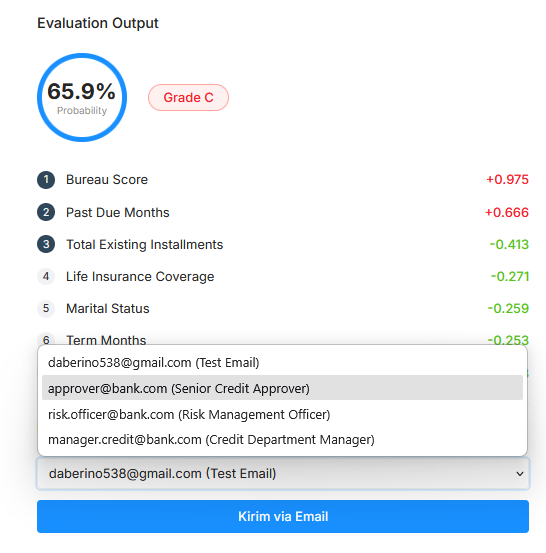
\includegraphics[width=0.80\textwidth]{bab4/MultipleEmailsent.png}
\caption{Pengiriman email konfirmasi ke beberapa staf bank terkait proses persetujuan kredit}
\label{fig:bab4_multiple_email_sent}
\end{figure}

Selain itu, sistem menyediakan formulir peminjaman yang disusun untuk mengikuti kebutuhan data pada proses pengajuan kredit. Formulir tersebut memuat atribut nasabah dan informasi pengajuan yang diperlukan agar data dapat diproses oleh pipeline, disimpan ke database, dan dianalisis oleh model risiko kredit. Tampilan formulir peminjaman ditunjukkan pada Gambar \ref{fig:bab4_form_peminjaman}.

\begin{figure}[H]
\centering
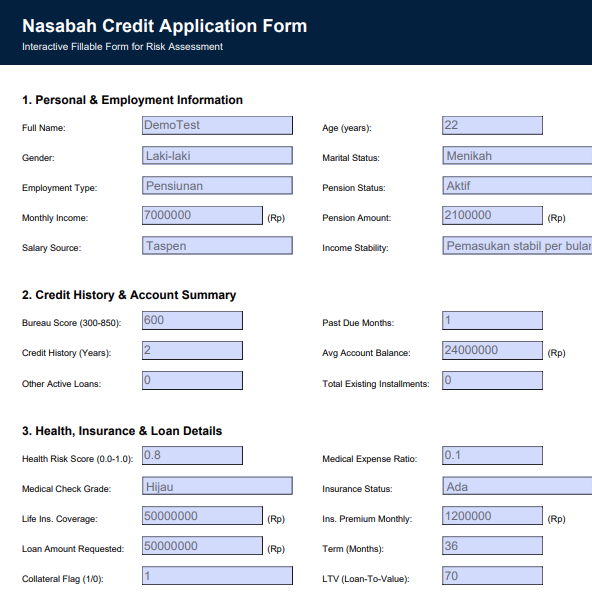
\includegraphics[width=0.92\textwidth]{bab4/FormPeminjaman.png}
\caption{Formulir peminjaman yang digunakan sebagai sumber data pengajuan kredit}
\label{fig:bab4_form_peminjaman}
\end{figure}

\begin{figure}[H]
\centering
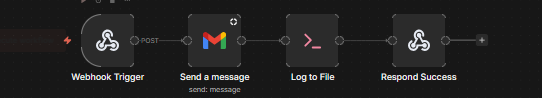
\includegraphics[width=0.92\textwidth]{bab4/Email_Sent_pipeline.png}
\caption{Workflow n8n untuk pengiriman email konfirmasi persetujuan kredit}
\label{fig:bab4_email_sent_pipeline}
\end{figure}

Hasil pengujian kedua workflow tersebut memperlihatkan bahwa n8n berperan sebagai komponen orkestrasi tambahan di luar retraining otomatis. Dengan adanya ingestion PDF dan pengiriman konfirmasi email, pipeline MLOps yang dibangun tidak hanya mencakup pelatihan, serving, dan monitoring model, tetapi juga mendukung integrasi proses bisnis kredit dari penerimaan dokumen hingga eskalasi keputusan kepada manusia.

\subsection{Evaluasi Aturan Bisnis Batas Usia dan Mitigasi Tenor Dinamis}
Sebelum aturan pembatasan usia pelunasan diterapkan pada modul \textit{serving}, sistem evaluasi risiko kredit sepenuhnya bergantung pada keluaran model XGBoost. Kondisi ini menimbulkan celah risiko bisnis karena model dapat meluluskan nasabah berusia lanjut, misalnya berusia 75 hingga lebih dari 80 tahun, dengan peringkat risiko baik dan probabilitas default yang rendah. Anomali tersebut muncul karena sebagian nasabah lanjut usia memiliki profil keuangan yang terlihat kuat bagi model, seperti aliran pendapatan pensiun yang stabil, skor kredit biro yang tinggi, rasio DTI yang rendah, serta status asuransi jiwa aktif.

Kelemahan tersebut menunjukkan bahwa model machine learning murni hanya menangkap korelasi matematis antarfitur, tetapi tidak secara eksplisit memahami risiko biologis dan batas kelayakan usia pelunasan. Sebagai contoh, nasabah berusia 75 tahun dengan profil pensiun stabil dapat dinilai rendah risiko oleh model, walaupun pengajuan tenor 10--15 tahun secara praktis dapat melewati batas usia pelunasan yang aman bagi institusi keuangan. Oleh karena itu, diperlukan lapisan logika bisnis tambahan agar hasil prediksi model tetap selaras dengan kebijakan manajemen risiko.

Untuk mengatasi kondisi tersebut, diterapkan sistem logika hibrida pada lapisan API. Sistem ini menghitung usia saat jatuh tempo dengan Persamaan \ref{eq:bab4_age_maturity}. Jika usia pelunasan melebihi 80 tahun, maka prediksi model dipotong atau \textit{bypass} sehingga sistem tidak memberikan persetujuan otomatis meskipun probabilitas default dari model tergolong rendah.

\begin{equation}
    \text{Usia Pelunasan} = \text{Usia Saat Pengajuan} + \frac{\text{Tenor (Bulan)}}{12}
    \label{eq:bab4_age_maturity}
\end{equation}

Mekanisme mitigasi tersebut dibagi ke dalam \textbf{tiga zona keputusan}:

\begin{enumerate}
    \item \textbf{Zona Lolos Batas Usia} --- kondisi ketika usia pelunasan $\leq$ 80 tahun. Pada zona ini, data tetap dikirimkan ke model XGBoost untuk memperoleh probabilitas \textit{default} dan \textit{risk grade} secara normal.

    \item \textbf{Zona Mitigasi Dinamis} --- kondisi ketika usia nasabah saat pengajuan masih di bawah 80 tahun, tetapi tenor yang diminta menyebabkan usia pelunasan melewati 80 tahun. Pada zona ini, sistem memberikan status Grade Undefined dan menghitung rekomendasi tenor maksimal secara dinamis menggunakan Persamaan \ref{eq:bab4_max_tenor}.

    \begin{equation}
        \text{Tenor Maksimal (Bulan)} = (80 - \text{Usia Saat Pengajuan}) \times 12
        \label{eq:bab4_max_tenor}
    \end{equation}

    Sebagai contoh, nasabah berusia 75 tahun yang mengajukan tenor 120 bulan akan direkomendasikan untuk menurunkan tenor maksimal menjadi 60 bulan. Jika nasabah memiliki asuransi jiwa aktif, sistem juga dapat memberikan rekomendasi dispensasi komite kredit berbasis perlindungan asuransi.

    \item \textbf{Zona \textit{Joint-Borrower}} --- kondisi ketika nasabah telah berusia 80 tahun atau lebih pada saat pengajuan. Pada zona ini, pengurangan tenor tidak lagi memadai karena sisa batas usia bernilai nol atau negatif. Sistem menyarankan alternatif pengajuan berbasis \textit{joint-income} atau \textit{co-borrower} dengan anggota keluarga inti yang lebih muda.
\end{enumerate}

Visualisasi batas keputusan mitigasi ditunjukkan pada Gambar \ref{fig:bab4_mitigation_boundary}. Gambar tersebut memperlihatkan bahwa sistem tidak hanya membedakan nasabah berdasarkan hasil prediksi model, tetapi juga berdasarkan kombinasi usia dan tenor. Area normal menunjukkan pengajuan yang masih dapat dievaluasi oleh model, sedangkan area mitigasi menunjukkan pengajuan yang membutuhkan pengurangan tenor, pertimbangan dispensasi, atau penahanan keputusan otomatis ketika batas usia tidak dapat dipenuhi.

\begin{figure}[H]
\centering
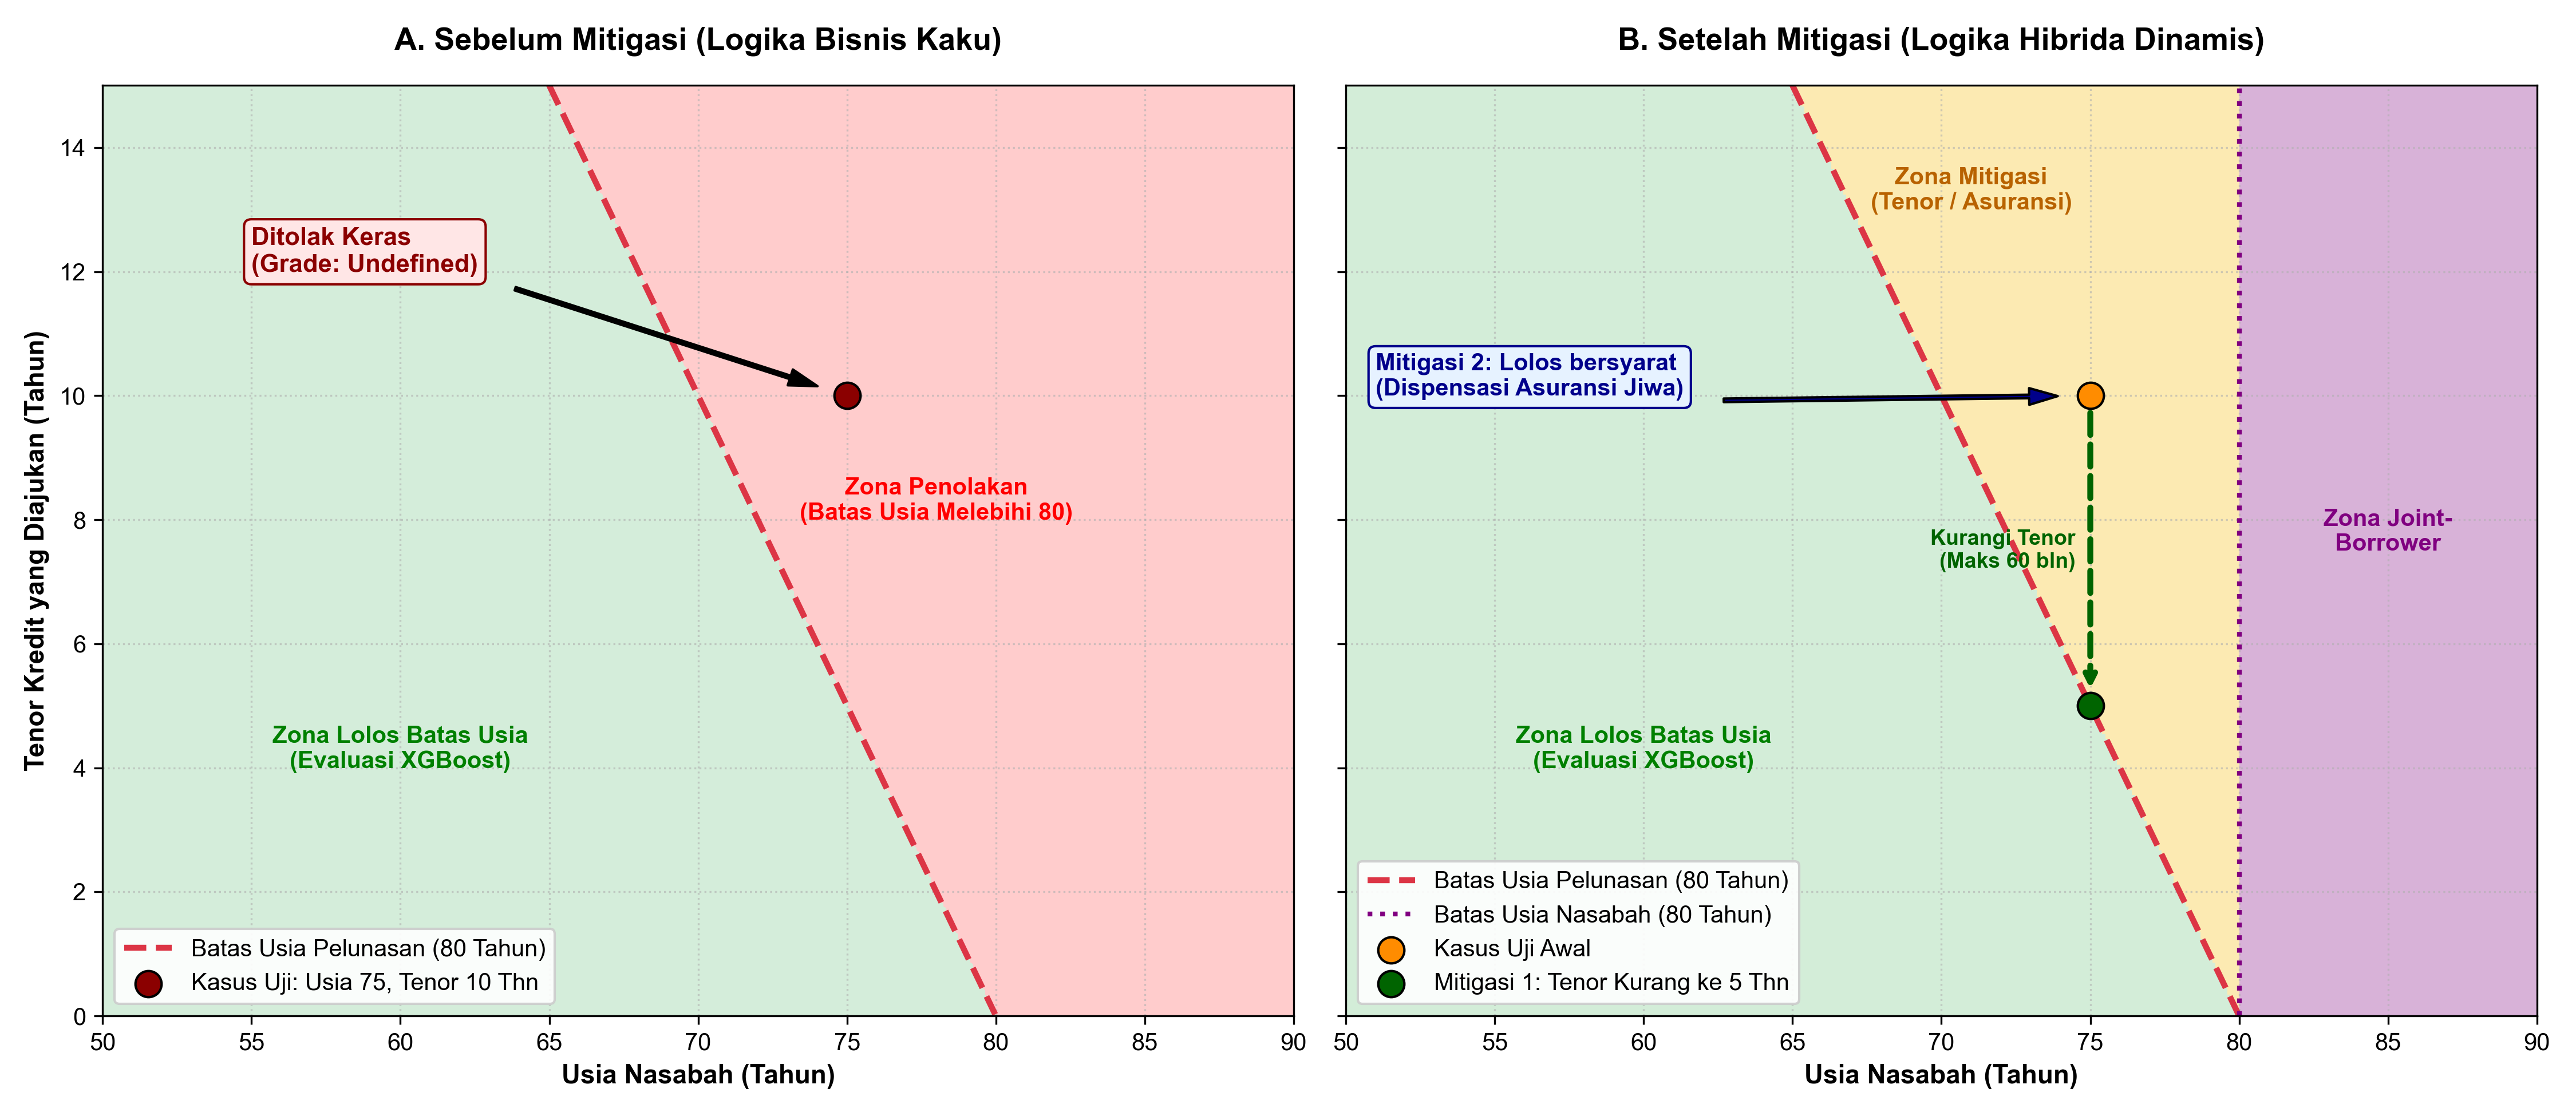
\includegraphics[width=0.82\textwidth]{bab4/mitigation_decision_boundary.png}
\caption{Visualisasi batas keputusan mitigasi usia dan tenor kredit}
\label{fig:bab4_mitigation_boundary}
\end{figure}

Setelah mekanisme ini diterapkan, sistem berhasil menyeimbangkan kecerdasan prediktif model dengan kepatuhan terhadap kebijakan risiko perbankan. Nasabah lanjut usia yang sebelumnya dapat lolos karena profil keuangannya terlihat baik kini terjaring oleh deteksi anomali usia pelunasan. Namun, sistem tidak langsung menolak secara kaku, melainkan memberikan rekomendasi terukur melalui pengurangan tenor atau pertimbangan asuransi jiwa kredit. Dengan demikian, aturan bisnis ini berfungsi sebagai lapisan pengaman tambahan yang membuat hasil inferensi model lebih realistis dan dapat diterapkan pada proses kredit operasional.

\section{Pengujian Deteksi Drift dan Retraining Otomatis}
\label{sec:bab4_drift_retraining}
Pengujian \textit{drift} dilakukan untuk memvalidasi mekanisme pemantauan distribusi data produksi pada modul drift\_monitor.py. Sistem yang dibangun menggunakan pendekatan \textbf{dual-trigger}, yaitu dua jalur pemicuan yang bekerja secara bersamaan: trigger berbasis jadwal setiap 7 hari dan trigger berbasis event saat data nasabah baru diinput. Pengujian difokuskan pada skenario terkontrol untuk membuktikan bahwa kedua mekanisme ini dapat mendeteksi pergeseran distribusi dan secara otomatis memicu proses retraining melalui webhook n8n.

\subsection{Pengujian Trigger Berbasis Jadwal}

Pada jalur ini, sistem secara terjadwal membandingkan distribusi fitur data produksi terkini terhadap distribusi data referensi menggunakan \textbf{Kolmogorov-Smirnov (KS) Test}. KS Test dipilih karena merupakan uji distribusi non-parametrik yang tidak memerlukan asumsi distribusi tertentu sehingga cocok untuk fitur tabular dengan distribusi campuran.

Skenario \textbf{stabil} dibandingkan dengan skenario \textbf{drift} yang mensimulasikan penurunan pendapatan sebesar 20\% dan peningkatan jumlah pinjaman sebesar 35\%, merepresentasikan kondisi makroekonomi yang memburuk. Hasil pengujian ditampilkan pada Tabel~\ref{tab:bab4_drift}.

\begin{table}[H]
\centering
\caption{Hasil pengujian deteksi drift menggunakan KS Statistic}
\label{tab:bab4_drift}
\begin{tabular}{|p{0.22\textwidth}|p{0.16\textwidth}|p{0.16\textwidth}|p{0.14\textwidth}|p{0.18\textwidth}|}
\hline
\textbf{Fitur} & \textbf{KS Stabil} & \textbf{KS Drifted} & \textbf{p-value} & \textbf{Tindakan} \\
\hline
\textit{monthly\_income} & 0,043 & 0,312 & $< 0{,}05$ & Webhook retrain dipicu \\
\hline
\textit{loan\_amount} & 0,038 & 0,287 & $< 0{,}05$ & Webhook retrain dipicu \\
\hline
\end{tabular}
\end{table}

Pada kondisi stabil, nilai KS-statistic kedua fitur berada di bawah 0,05 dengan \textit{p-value} $> 0{,}05$, menunjukkan bahwa distribusi produksi tidak berbeda signifikan dari distribusi referensi --- layanan API tetap berjalan normal. Pada kondisi drifted, nilai KS-statistic melonjak melampaui ambang signifikansi $\alpha = 0{,}05$, sehingga sistem mengklasifikasikan kondisi sebagai \textit{drift terdeteksi} dan mengeksekusi fungsi trigger\_retrain untuk mengirim \textit{HTTP POST} ke server n8n.

\subsection{Pengujian Trigger Berbasis Event}

Jalur kedua bekerja secara independen. Setiap kali endpoint POST /api/nasabah menerima data nasabah baru, sistem menambah penghitung kumulatif data baru sejak model terakhir dilatih. Apabila penghitung melampaui \textit{ingestion threshold} yang dikonfigurasi, \textit{workflow} n8n memicu evaluasi dan retraining secara langsung tanpa menunggu jadwal mingguan.

Hal ini menunjukkan bahwa pipeline MLOps mampu membentuk mekanisme \textit{closed-loop automation}: model tidak hanya digunakan untuk inferensi, tetapi juga dipantau dan diperbarui secara responsif --- baik oleh perubahan distribusi data (schedule trigger) maupun oleh volume data baru yang masuk (event trigger).

Implementasi orkestrasi retraining otomatis pada n8n ditunjukkan pada Gambar \ref{fig:bab4_n8n_workflow}. Workflow tersebut memuat beberapa komponen utama, yaitu \textit{Schedule Trigger} untuk eksekusi berkala, \textit{Webhook} untuk menerima pemicu eksternal dari modul drift monitoring, node eksekusi perintah untuk menjalankan proses pemeriksaan atau pelatihan ulang, node kondisional untuk menentukan apakah retraining diperlukan, serta \textit{HTTP Request} untuk menghubungkan proses otomasi dengan layanan terkait. Dengan struktur tersebut, proses monitoring dan retraining dapat dijalankan secara otomatis tanpa intervensi manual penuh.

\begin{figure}[H]
\centering
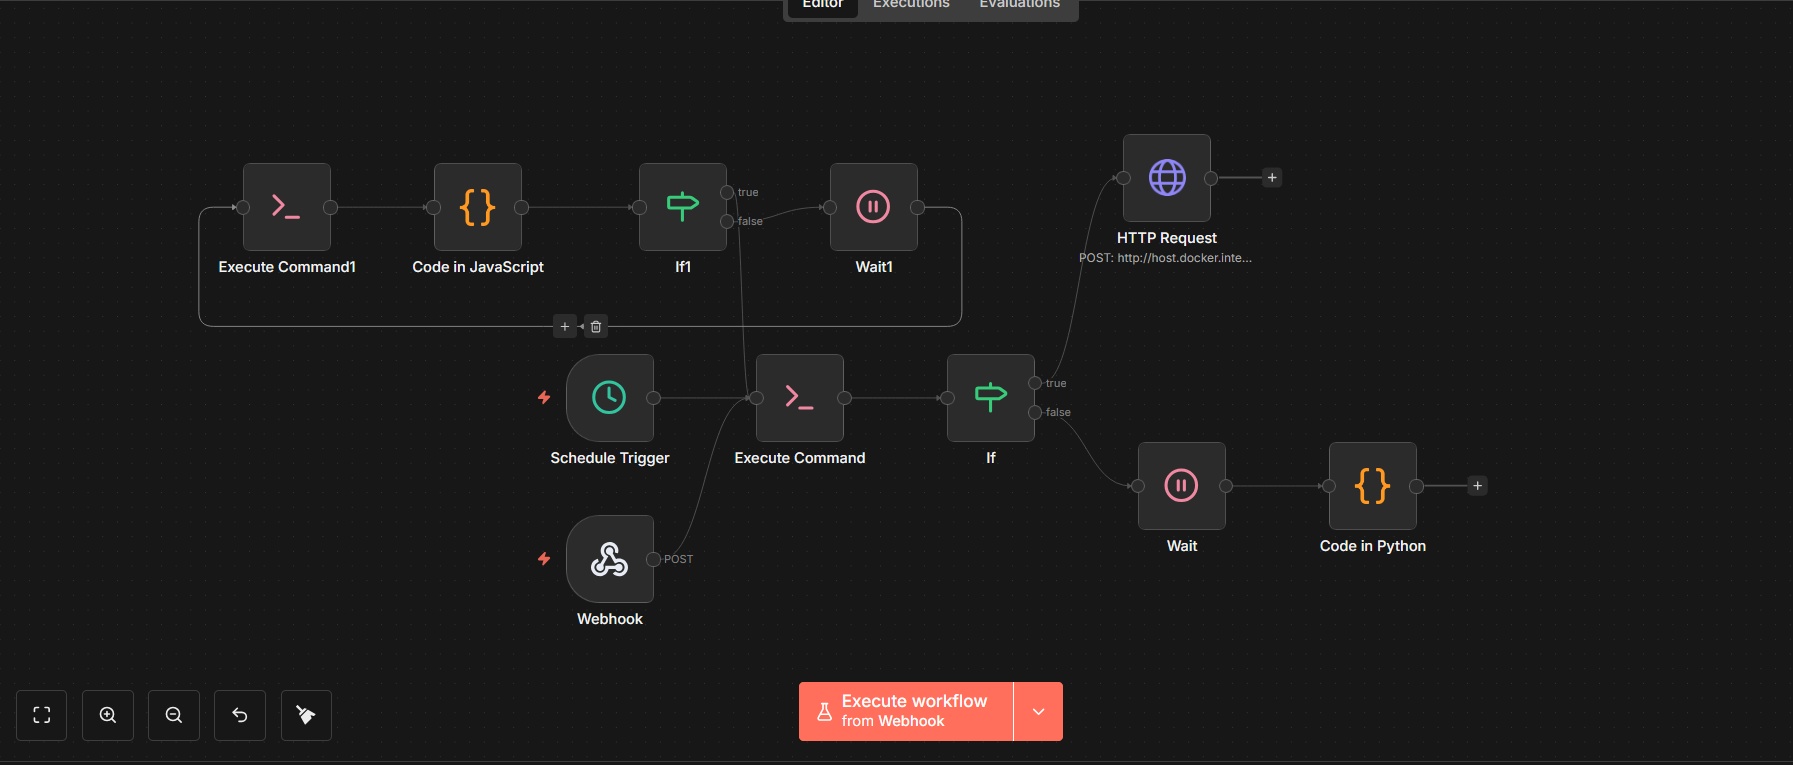
\includegraphics[width=0.92\textwidth]{bab4/Screenshot 2026-05-25 171559.png}
\caption{Workflow n8n untuk orkestrasi monitoring drift dan retraining otomatis}
\label{fig:bab4_n8n_workflow}
\end{figure}

\section{Analisis Deskriptif}
\label{sec:bab4_evaluasi_kritis}
Meskipun hasil pengujian menunjukkan bahwa pipeline MLOps telah mampu menjalankan otomasi pelatihan, deployment, monitoring drift, dan integrasi aturan bisnis, sistem ini masih memiliki beberapa batasan jika dilihat dari sudut pandang manajemen risiko riil. Evaluasi kritis ini penting karena sistem penilaian kredit tidak hanya harus akurat secara teknis, tetapi juga harus aman secara operasional dan dapat dipertanggungjawabkan secara ekonomi.

\subsection{Kebutuhan Human-in-the-Loop pada Zona Ambang}
Meskipun sistem telah memiliki mekanisme konfirmasi email untuk mendukung \textit{human-in-the-loop}, pengujian pada zona ambang tetap membutuhkan aturan eskalasi yang lebih eksplisit. Pada nilai probabilitas gagal bayar atau \textit{Probability of Default} (PD) yang berada pada zona ambang, misalnya 40\% hingga 60\%, tingkat ketidakpastian model relatif tinggi. Jika kasus pada rentang ini tidak secara otomatis diberi tanda \textit{mandatory human review}, maka sistem tetap berpotensi menghasilkan kesalahan klasifikasi, baik berupa \textit{false positive} maupun \textit{false negative}.

Dalam praktik operasional perbankan, zona abu-abu tersebut sebaiknya tidak diperlakukan sebagai keputusan otomatis. Mekanisme email yang telah tersedia perlu diperkuat dengan \textit{review flag} berbasis threshold agar pengajuan pada zona ambang otomatis dialihkan kepada analis kredit atau \textit{credit underwriter}. Dengan demikian, hasil prediksi model dapat dikombinasikan dengan penilaian kualitatif, seperti stabilitas pekerjaan, kondisi keluarga, dokumen pendukung, dan informasi tambahan yang tidak selalu tercermin di dalam fitur model.

\subsection{Beban Finansial Spesifik yang Tidak Sepenuhnya Tercermin pada Risk Grade}
Berdasarkan penelaahan deskriptif terhadap sampel data nasabah, terdapat celah antara validasi lapangan dan keluaran model. Sebagai contoh, pada sampel nasabah di Tabel \ref{tab:nasabah_normal}, terdapat nasabah dengan pendapatan bulanan sekitar Rp3.285.278 dan rasio pengeluaran medis yang tinggi. Jika rasio pengeluaran medis mencapai 42,09\%, maka sekitar Rp1,38 juta per bulan digunakan untuk biaya medis rutin. Secara operasional, beban tersebut dapat bertindak sebagai \textit{fixed commitment} yang mengurangi kapasitas membayar atau \textit{repayment capacity}.

Kondisi serupa juga dapat terjadi pada pengeluaran non-medis yang bersifat mengikat, seperti biaya pendidikan anak berkebutuhan khusus atau kewajiban keluarga lain yang tidak selalu tertangkap secara eksplisit oleh model. Dalam beberapa kasus, model masih dapat memberikan grade yang relatif moderat karena didorong oleh fitur lain seperti \textit{bureau\_score} yang tinggi. Hal ini menunjukkan bahwa catatan manual dari petugas Kredit Validator tetap perlu menjadi bagian dari proses intervensi, terutama ketika terdapat beban finansial spesifik yang tidak cukup direpresentasikan oleh variabel model.

Dengan demikian, keluaran model sebaiknya diposisikan sebagai alat bantu keputusan, bukan pengganti penuh proses validasi kredit. Pipeline perlu dikembangkan agar dapat menerima \textit{manual override flag} atau catatan validator sebagai sinyal tambahan untuk menurunkan grade, mengubah status menjadi Undefined, atau mengalihkan kasus ke proses review manual.

\subsection{Kerentanan Subjektivitas pada Proses WoE Binning}
Transformasi \textit{Weight of Evidence} (WoE) terbukti membantu stabilitas fitur dan mendukung interpretabilitas model. Namun, proses pembentukan interval atau \textit{binning} pada variabel numerik tetap memiliki unsur sensitivitas metodologis. Perbedaan metode binning, seperti \textit{equal width}, \textit{equal frequency}, atau binning berbasis aturan bisnis, dapat menghasilkan batas interval yang berbeda dan pada akhirnya mengubah nilai WoE.

Jika batas bin ditentukan semata-mata oleh algoritma tanpa validasi dari komite risiko, model dapat menjadi benar secara teknis tetapi kurang tepat secara ekonomi. Sebagai contoh, perubahan kecil pada batas kelompok \textit{bureau\_score} dapat mengubah interpretasi risiko dan memengaruhi skor akhir nasabah. Oleh karena itu, proses binning perlu divalidasi tidak hanya berdasarkan metrik statistik, tetapi juga berdasarkan kewajaran bisnis dan kebijakan risiko lembaga keuangan.

Batasan ini menunjukkan bahwa implementasi pipeline MLOps pada domain kredit perlu dilengkapi dengan tata kelola model yang kuat. Setiap perubahan fitur, binning WoE, threshold PD, aturan grading, dan mekanisme retraining sebaiknya terdokumentasi, ditinjau, dan disetujui oleh pihak yang bertanggung jawab terhadap risiko model.

\subsection{Dependensi Infrastruktur pada Lingkungan Lokal}
Pengujian sistem dilakukan pada lingkungan lokal menggunakan Docker dan Docker Compose. Konfigurasi ini memadai untuk validasi prototipe karena seluruh komponen seperti FastAPI, MLflow, n8n, database SQLite, dan file log dapat dijalankan dalam satu lingkungan pengujian. Namun, untuk skenario produksi skala penuh, ketergantungan pada konektivitas lokal antarservice dan penyimpanan file lokal perlu diperhatikan karena dapat menjadi titik kegagalan ketika jumlah pengguna, volume prediksi, atau kebutuhan audit meningkat.

Pada implementasi produksi, database SQLite dapat dipertimbangkan untuk dimigrasikan ke sistem basis data server seperti PostgreSQL, sedangkan log inferensi sebaiknya disimpan pada penyimpanan terpusat atau terdistribusi. Selain itu, komunikasi antarservice perlu dilengkapi autentikasi, pemantauan ketersediaan, serta strategi backup dan recovery. Dengan demikian, sistem tidak hanya siap secara fungsional, tetapi juga lebih kuat dari sisi reliabilitas dan tata kelola operasional.

\section{Ringkasan Bab}
\label{sec:bab4_ringkasan}
Bab ini telah menguraikan hasil pengujian sistem mulai dari preprocessing, penanganan imbalance, pelatihan model, evaluasi performa, interpretabilitas, quality gate data sintetis, API serving, database nasabah, ingestion PDF, konfirmasi email HITL, aturan bisnis, hingga deteksi drift. Hasil pengujian menunjukkan bahwa model XGBoost memperoleh AUC 0,8262 dengan keseimbangan presisi dan recall yang baik. Transformasi WoE dan seleksi IV membantu memperkuat dasar pemilihan fitur, sedangkan SHAP memberikan transparansi terhadap faktor yang memengaruhi prediksi.

Selain performa model, hasil pengujian juga menunjukkan bahwa data sintetis lolos quality gate utilitas dan privasi, layanan FastAPI mampu mengembalikan prediksi beserta penjelasan, database mendukung CRUD dan audit email, workflow n8n mendukung retraining serta ingestion PDF, aturan bisnis dapat mencegah keputusan yang melanggar kebijakan, dan sistem drift monitoring mampu memicu retraining otomatis. Dengan demikian, sistem yang dikembangkan tidak hanya memenuhi kebutuhan pemodelan prediktif, tetapi juga menunjukkan kesiapan sebagai pipeline MLOps yang operasional, dapat diaudit, dan tetap membutuhkan tata kelola manusia pada kasus yang berisiko.

\cleardoublepage
\chapter{PENUTUP}
\label{sec:chap5_tutup}

Bab ini menyajikan kesimpulan dan saran dari perancangan serta pengujian sistem \textit{Credit Risk Scoring} berbasis \textit{Machine Learning Operations} (MLOps).

\section{Kesimpulan}
\label{sec:sec5_kesimpulan}
Berdasarkan hasil penelitian dan pengujian, diperoleh beberapa kesimpulan sebagai berikut:

\begin{enumerate}
    \item Penelitian ini berhasil merancang pipeline MLOps untuk operasionalisasi model prediktif risiko kredit, mulai dari pembentukan data sintetis, pra-pemrosesan, pelatihan model, deployment API, interpretabilitas, hingga otomasi pelatihan ulang berkelanjutan (Continuous Training).

    \item Penggunaan data sintetis memungkinkan penelitian risiko kredit dilakukan tanpa menggunakan data nasabah riil. Dataset yang dibangun telah memuat atribut demografis, finansial, histori kredit, asuransi, produk pinjaman, serta parameter risiko yang relevan terhadap proses \textit{credit scoring}.

    \item Tahap pra-pemrosesan menggunakan WoE, IV, dan SMOTE membantu meningkatkan kualitas fitur serta menangani ketidakseimbangan kelas. Model XGBoost yang dikembangkan memperoleh AUC sebesar 0,8262, precision 0,8024, recall 0,7549, dan F1-score 0,7779.

    \item Integrasi SHAP, FastAPI, sistem grading, dan aturan bisnis membuat hasil prediksi lebih transparan dan operasional. Kategori Undefined juga membantu mencegah keputusan otomatis pada kasus yang membutuhkan pengecekan manual, seperti usia pelunasan yang melebihi batas kebijakan.

    \item Implementasi MLflow dan n8n menunjukkan bahwa proses pelacakan eksperimen, \textit{Continuous Training}, dan pemicuan retraining dapat diotomatisasi. Dengan demikian, sistem yang dibangun dapat menjadi prototipe awal pipeline MLOps untuk model risiko kredit.
\end{enumerate}

Secara keseluruhan, penelitian ini menunjukkan bahwa kombinasi model prediktif, interpretabilitas, aturan bisnis, dan otomasi MLOps dapat mendukung sistem penilaian risiko kredit yang lebih terstruktur. Namun, karena data yang digunakan masih bersifat sintetis, sistem ini tetap memerlukan validasi lebih lanjut sebelum diterapkan pada keputusan kredit riil.

\section{Saran}
\label{sec:sec5_saran}
Beberapa saran untuk pengembangan penelitian selanjutnya adalah sebagai berikut:

\begin{enumerate}
    \item Melakukan validasi menggunakan data historis riil yang telah dianonimkan agar performa model dapat diuji pada kondisi portofolio kredit yang sebenarnya.

    \item Mengembangkan proses pembentukan data sintetis dan membandingkan model XGBoost dengan pendekatan lain, seperti Logistic Regression, Random Forest, LightGBM, CatBoost, atau model berbasis \textit{scorecard}.

    \item Menyempurnakan aturan bisnis dan sistem grading dengan mempertimbangkan kebijakan internal bank, jenis produk kredit, batas usia, tenor, asuransi, serta skema \textit{co-borrower}.

    \item Memperkuat pipeline MLOps dengan audit trail, monitoring performa, validasi otomatis model baru, keamanan API, dan dashboard operasional agar sistem lebih siap digunakan pada lingkungan produksi.
\end{enumerate}

\cleardoublepage
\input{Init/DaftarPustaka.tex}
\cleardoublepage
\begin{center}
  \Large
  \textbf{BIOGRAFI PENULIS}
\end{center}

\addcontentsline{toc}{chapter}{BIOGRAFI PENULIS}

\vspace{2ex}

\begin{wrapfigure}{L}{0.3\textwidth}
  \centering
  \vspace{-3ex}
  % Ubah file gambar berikut dengan file foto dari mahasiswa
  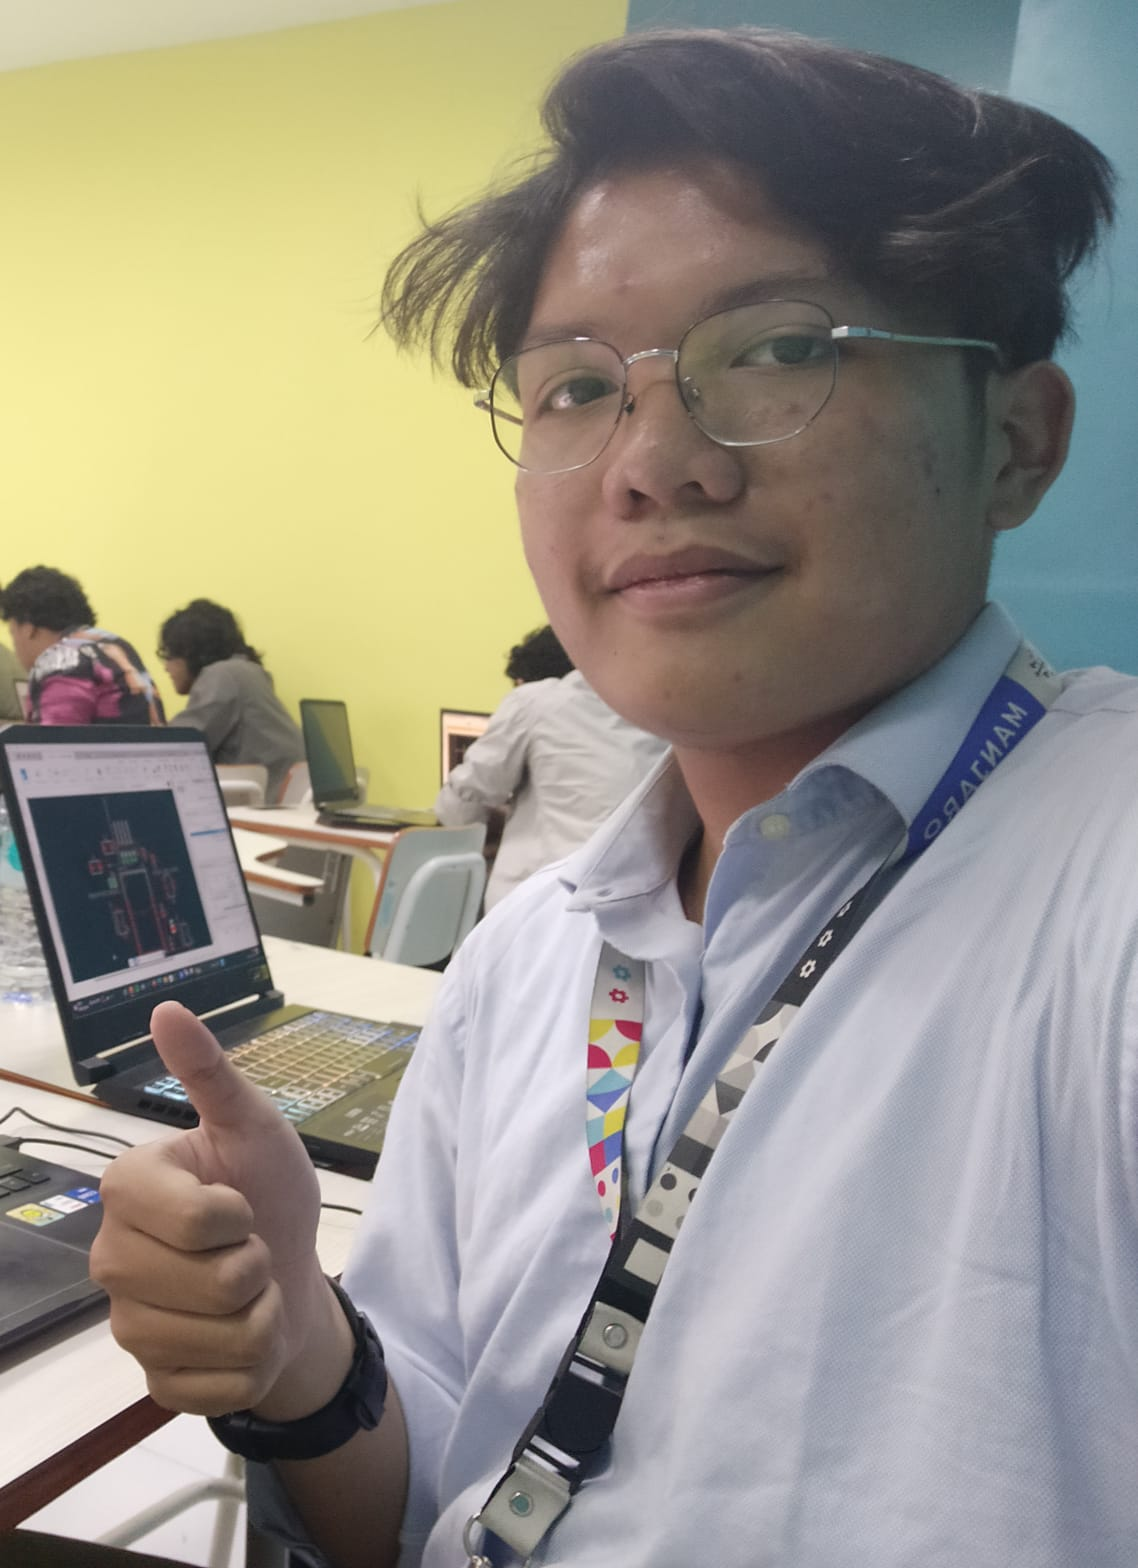
\includegraphics[width=0.3\textwidth]{BiografiPenulis/foto-formal.png}
  \vspace{-4ex}
\end{wrapfigure}

% Ubah kalimat berikut dengan biografi dari mahasiswa
\name{}, atau yang biasa dikenal sebagai Imanuel Daulat, merupakan mahasiswa Program Studi Teknik Komputer, Departemen Teknik Komputer, Fakultas Teknologi Elektro dan Informatika Cerdas, Institut Teknologi Sepuluh Nopember (ITS) angkatan 2022. Saat ini penulis menempuh perkuliahan pada semester akhir dan memiliki ketertarikan pada bidang analisis data, kecerdasan buatan, serta \textit{Machine Learning Operations} (MLOps).

Selama masa studi, penulis aktif mengembangkan kompetensi teknis yang berkaitan dengan pengolahan data, pengembangan model berbasis \textit{machine learning}, dan penerapan sistem berbasis data untuk mendukung proses pengambilan keputusan. Ketertarikan tersebut semakin berkembang melalui pengalaman profesional penulis di industri saat menjalani peran sebagai IT Operations \& Data Analyst Intern di Bank Mandiri Taspen, Jakarta. Dalam pengalaman tersebut, penulis berfokus pada optimalisasi query SQL Server serta pengembangan dashboard analitik menggunakan Tableau untuk mendukung kebutuhan analisis pada divisi internal perusahaan.

Pada penelitian tugas akhir ini, penulis mengangkat topik perancangan dan implementasi pipeline \textit{Machine Learning Operations} (MLOps) untuk operasionalisasi model prediktif risiko kredit. Topik ini dipilih karena sejalan dengan minat penulis pada bidang analisis data, kecerdasan buatan, dan penerapan sistem data di industri keuangan. Melalui penelitian ini, penulis berharap hasil yang dikembangkan dapat memberikan kontribusi awal terhadap penerapan sistem \textit{credit risk scoring} yang lebih terstruktur, transparan, dan adaptif terhadap perubahan data.

\cleardoublepage
\end{document}
